% -*- Mode:TeX -*-


% IMPORTANT: The official thesis specifications are available at:
%
%            http://libraries.mit.edu/archives/thesis-specs/


% **************************************************************************************************************
% A Classic Thesis Style
% An Homage to The Elements of Typographic Style
%
% Copyright (C) 2015 André Miede http://www.miede.de
%
% If you like the style then I would appreciate a postcard. My address 
% can be found in the file ClassicThesis.pdf. A collection of the 
% postcards I received so far is available online at 
% http://postcards.miede.de
%
% License:
% This program is free software; you can redistribute it and/or modify
% it under the terms of the GNU General Public License as published by
% the Free Software Foundation; either version 2 of the License, or
% (at your option) any later version.
%
% This program is distributed in the hope that it will be useful,
% but WITHOUT ANY WARRANTY; without even the implied warranty of
% MERCHANTABILITY or FITNESS FOR A PARTICULAR PURPOSE.  See the
% GNU General Public License for more details.
%
% You should have received a copy of the GNU General Public License
% along with this program; see the file COPYING.  If not, write to
% the Free Software Foundation, Inc., 59 Temple Place - Suite 330,
% Boston, MA 02111-1307, USA.
%
% **************************************************************************************************************
\RequirePackage{fix-cm} % fix some latex issues see: http://texdoc.net/texmf-dist/doc/latex/base/fixltx2e.pdf
\documentclass[ twoside,openright,titlepage,numbers=noenddot,headinclude,%1headlines,% letterpaper a4paper
                footinclude=true,cleardoublepage=empty,abstractoff, % <--- obsolete, remove (todo)
                BCOR=5mm,paper=letter,fontsize=11pt,%
                ngerman,american,%
                ]{scrreprt}


% ***************************************
% Note: Make all your adjustments in here
% ***************************************
\input{classicthesis-config}

\numberwithin{equation}{chapter}
\numberwithin{figure}{chapter}
\numberwithin{table}{chapter}

\usepackage{nomenlev}\makenomen
\usepackage{verbatim}

\newcommand{\erf}{\text{erf}}
\newcommand{\atan}{\tan^{-1}}
\newcommand{\vect}{\boldsymbol}
\newcommand{\cross}{\times}
\newcommand{\ts}{\textsuperscript}
\newcommand{\diiid}{\mbox{DIII-D}}
\newcommand{\sinc}{\text{sinc}}


% **************
% Bibliographies
% **************
% \addbibresource{Bibliography.bib}
% \addbibresource[label=ownpubs]{AMiede_Publications.bib}


% ***********
% Hyphenation
% ***********
%\hyphenation{put special hyphenation here}


% \includeonly{Chapters/ToroidalCorrelation/ToroidalCorrelation}
% \includeonly{Chapters/InterferometricMethods/InterferometricMethods}


\begin{document}


\frenchspacing
\raggedbottom
\selectlanguage{american} % american ngerman
%\renewcommand*{\bibname}{new name}
%\setbibpreamble{}
%\pagenumbering{roman}
\pagestyle{plain}


% ***********
% Frontmatter
% ***********
\include{FrontBackmatter/Cover}
\section*{Acknowledgments}
I would like to thank the members of the \diiid\space PCI group.
My advisor, Professor Miklos Porkolab,
never lost faith in my ability to complete this project, and
he exercised patience as I developed into an independent scientist.
Chris Rost, my day-to-day supervisor,
spent countless hours with me in the \diiid\space ``pit'',
taught me the importance of being thorough and precise, and
brilliantly identified the origin of the noise crippling our system,
without which I may not have completed this project.
Alessandro Marinoni spent nearly as many hours working with me in the pit, and
he also ran the TGLF simulations
that tie nicely into the multiscale turbulence measurements
described in this thesis.

I would also like thank numerous other people from MIT.
In particular, Earl Marmar and John Belcher
served on my committee and slogged through
this tome of a thesis.
Earl also generously supported the last $3.5$ years of my studies
through the PSFC's MFE collaboration funds.
Conversations with Jim Irby were enlightening and
helped diagnose the enormous noise in our system.
Jessica Coco happily arranged much of my graduate travel,
substantially reducing the stress and bureaucracy of reimbursement.
Carol Arlington kept Miklos's exceptionally busy schedule organized,
ensuring he always had sufficient time to meet with me.
Jerry Hughes stood up for me when no one else would.
The graduate students of the PSFC were an enormous support network
during my first three years of graduate school;
of particular note are
Ian Faust,
Mark Chilenski (my officemate, who taught me a ton),
John Walk,
Choongki Sung (who subsequently became my \diiid\space control-room confidant),
and Ted Golfinopoulos.
Naoto Tsujii and Paul Ennever introduced me to the C-Mod PCI system.
The closure of C-Mod brought some dark times, but,
like a phoenix rising from the ashes,
I see a bright future for the PSFC, and
I am excited to see where everyone takes it.

I would additionally like to thank several people at \diiid,
where I spent the last $4.5$ years of my graduate studies.
Mike Van Zeeland and Tom Carlstrom,
the local interferometer gurus,
were always happy to share their extensive knowledge
of interferometry with me.
Daniel Finkenthal similarly shared his RF expertise and
provided \emph{pro bono} an automatic gain control amplifier, which
is crucial to the operation of our interferometer.
On several occasions, David Pace lent us channels
on his high-frequency $200$ MSPS digitizer, which
ultimately allowed Chris Rost to identify
the origin of the noise crippling our system.
R\'{e}jean Boivin checked in with me often
to ensure I was not ``falling between the cracks''.
Bob Pinsker fostered a collegiate atmosphere,
regularly hosting \diiid's student/postdoc seminar series, and
he also lent us the high-power RF amplifier needed to drive our AOM.
Lupe Cerda was always happy to help me navigate the \diiid\space bureaucracy.
The \diiid\space ``lunch crew'',
consisting of a hodge podge of graduate students, postdocs, and scientists
from multiple institutions,
always made for an entertaining lunch;
of particular note are
Matthias Kn{\"o}lker,
Mitchell Clement,
``Staff'' Tyler Abrams,
Ryan Sweeney,
Brent Covele, and
Wilkie Choi.
The short-lived ``Monday runday'' group
helped re-ignite my passion for running and
introduced me to running along the picturesque bluffs of La Jolla.

The Stewardship Science Graduate Fellowship (SSGF) program
generously supported the first $4$ years of my graduate study.
The Krell Institute, which administered the SSGF program, and
Lucille Kilmer in particular
were always a pleasure to interact with.

From Riverside, to Boston, to San Diego,
I have been blessed with some truly amazing friends.
John Paul Issa, you were there at the beginning, and
you were there at the end;
I feel like we have both been to our own personal hell and back, and
I am confident that the future is now bright.
You have always told it to me straight, but
you have never left me feeling bad.
Riley and Julia Takano, you make being responsible adults look so easy;
even a few hours with both of you has been enough to cure the lab blues.
Steven Warneke, it has been a long time
since our ``Titans of Industry'' talk and
our paths have swerved a bit since then, but
our friendship has only grown;
Madeline, I am so happy you found him and
are (mostly) keeping him out of trouble.
Rachel Cheong, you know me better than most and
still accept me for who I am;
you are beautiful inside and out.
Ian Faust, you made $881$ Mass Ave home, and
you truly helped me come into my own.
From Coachella to Oktoberfest,
you have never said no to adventure;
``unfortunately'', this has currently led you to Munich, but
even this has not put a wedge between us.
Alex Guo, you lead by example, and
you have a heart of gold.
Jason Ramapuram and Barbara Sandoval,
the kindness and friendship you both showed me
when I moved to San Diego
far exceeded my expectations;
your around-the-world adventures amaze and inspire me, but
I selfishly still wish you were in San Diego.
Matthias Kn{\"o}lker, from our off-hand introduction at lab
to where we are now, who could have guessed?
The only things that surprise me
more than your intuition and your humor
are your friendship and your loyalty.
Theresa Wilks, your optimism is infections, and
your laughter can move mountains.
Darren Burton \& co. (i.e.\ Scott and Andrew),
thanks for so many good times, good food, and
laughter inducing situations over the last year.

Finally, my family has always been the cornerstone of my life.
Cory, you've grown from being
my little brother to one of my best friends.
Your passions for astronomy and space exploration
have helped me remember why I got into science in the first place.
Thanks for never letting me forget where I came from.
Mom and Dad, you have been my number one fans since day one.
When I celebrated, you celebrated, and when I cried, you cried.
At this point, you are probably almost as well-versed in this thesis as I am.
Thank you for all of your love, support, and encouragement.
This thesis is dedicated to both of you.

This work was supported by
the U.S. Department of Energy,
Office of Science,
Office of Fusion Energy Sciences
under Award Numbers
DE-FG$02$-$94$ER$54235$,
DE-FC$02$-$04$ER$54698$, and
DE-FC$02$-$99$ER$54512$ and
the U.S. Department of Energy,
National Nuclear Security Administration,
Stewardship Science Graduate Fellowship program,
which is provided under grant number DENA$002135$.

\pagestyle{scrheadings}
\cleardoublepage\include{FrontBackmatter/Contents}


% **********
% Mainmatter
% **********
\cleardoublepage\pagenumbering{arabic}
\chapter{Introduction}


\section{Fusion energy}
Fusion is the energy of the sun and stars, and,
for the better part of the last century,
man has been striving to replicate this process
in a controlled manner here on earth
for a source of safe, clean, virtually inexhaustible source of energy.


\section{Tokamak fusion}
\subsection{Turbulent transport}
\subsection{Energetic-particle confinement}


\section{Interferometry}


\section{Thesis outline}
The remainder of this thesis is organized as follows:

\begin{itemize}
  \item Chapter 2 discusses the theory of optical interferometric methods
    in the context of measuring tokamak-plasma-density fluctuations.
    The laser-plasma interaction is quantified via
    Fraunhofer scalar-diffraction theory, and
    the resulting diffracted field is imaged on a square-law detector.
    Interfering the imaged field with a known reference field
    produces measurable intensity fluctuations;
    the specification of this reference field
    defines the interferometric method.
    Details of two particular interferometric methods ---
    external-reference-beam interferometry and
    phase contrast imaging (PCI) ---
    are discussed, with an emphasis on
    their dynamic ranges and spatiotemporal bandwidths.
  \item Chapter 3
\end{itemize}


\section{Units}

\chapter{Interferometric methods for tokamak-plasma fluctuations}
\label{ch:InterferometricMethods}
Interferometric methods exploit the interaction of
electromagnetic waves with a plasma
to ascertain properties of the plasma's density.
Because surveying every flavor of interferometric method
exceeds the scope of this work,
only the interferometric methods
of direct relevance to this work ---
external reference-beam interferometry and phase contrast imaging (PCI) ---
are discussed in detail.
Further, the emphasis is diagnosis of the plasma's density fluctuations
rather than its equilibrium density.
The overview of optical interferometry in
Section~\ref{sec:Introduction:OpticalInterferometry}
is mandatory background for this chapter.
While Section~\ref{sec:Introduction:OpticalInterferometry}
cavalierly assumes various forms for the interfering radiation fields,
this chapter provides first-principles descriptions
of the laser-plasma interaction and optical systems needed
to produce these radiation fields.

Below, Section~\ref{sec:InterferometricMethods:EM_waves_in_plasma}
examines the propagation of electromagnetic waves through a ``cold'' plasma
and derives an expression for the plasma-induced phase delay.
Section~\ref{sec:InterferometricMethods:Gaussian_beam_diffraction} reveals that
plasma-density fluctuations weakly upscatter and downscatter
an incident Gaussian probe beam, while
Section~\ref{sec:InterferometricMethods:imaging} describes
how an imaging system manipulates these scattered beams.
Section~\ref{sec:InterferometricMethods:interferometry} shows that
interfering the imaged probe radiation with an external reference beam
is an effective technique for diagnosing plasma-density fluctuations and
discusses the relative merits of homodyne versus heterodyne detection.
Section~\ref{sec:InterferometricMethods:pci} details the principles of
phase contrast imaging (PCI),
which does away with an external reference beam and
instead spatially filters the scattered and unscattered beams
to produce an informative interference signal.
Section~\ref{sec:InterferometricMethods:selection}
concludes the chapter by synthesizing the preceding results and
discussing the strengths and limitations of each interferometric technique.


\section{Electromagnetic waves in a plasma}
\label{sec:InterferometricMethods:EM_waves_in_plasma}
A great deal can be learned about a plasma
by probing it with electromagnetic waves.
Sections~\ref{sec:InterferometricMethods:EM_waves_in_plasma:derivation_of_wave_equation}---
\ref{sec:InterferometricMethods:EM_waves_in_plasma:cold_plasma_dispersion_relation}
derive the index of refraction $N$ for a cold, homogeneous plasma.
Section~\ref{sec:InterferometricMethods:EM_waves_in_plasma:propagation_in_inhomogeneous_medium}
extends these results to inhomogeneous plasmas via the WKB approximation and
assesses the validity of this approach for
a CO$_2$ probe beam in a typical tokamak plasma, and
Section~\ref{sec:InterferometricMethods:EM_waves_in_plasma:plasma_induced_phase_delay}
computes the resulting plasma-induced phase delay.


\subsection{Derivation of the wave equation}
\label{sec:InterferometricMethods:EM_waves_in_plasma:derivation_of_wave_equation}
The electric field $\vect{E}$ and the magnetic field $\vect{B}$
of an electromagnetic wave are coupled via Faraday's law
\begin{equation}
  \nabla \cross \vect{E}
  =
  - \frac{\partial \vect{B}}{\partial t}
  \label{eq:InterferometricMethods:Faradays_law}
\end{equation}
and Ampere's law
\begin{equation}
  \nabla \cross \vect{B}
  =
  \mu_0 \vect{J}
  +
  \mu_0 \epsilon_0 \frac{\partial \vect{E}}{\partial t},
  \label{eq:InterferometricMethods:Amperes_law}
\end{equation}
where $\epsilon_0$ is the permittivity of free space,
$\mu_0$ is the permeability of free space, and
$\vect{J}$ is the current density~\cite[Sec.~I.1]{jackson_E&M}.
Note that (\ref{eq:InterferometricMethods:Faradays_law}) and
(\ref{eq:InterferometricMethods:Amperes_law}) are the vacuum formulations
of Faraday's law and Ampere's law;
however, they can still be used to describe
an electromagnetic wave's propagation through a medium
\emph{if} that medium's electromagnetic properties
are explicitly accounted for in the current density $\vect{J}$
\cite[Sec.~I.4]{jackson_E&M}\cite[Sec.~4.1]{hutchinson_diagnostics}.
Now, taking the curl of Faraday's law and
then using Ampere's law to eliminate $\vect{B}$
yields the electric field's wave equation
\begin{equation}
  \nabla^2 \vect{E}
  -
  \frac{1}{c^2} \frac{\partial^2 \vect{E}}{\partial t^2}
  =
  \nabla(\nabla \cdot \vect{E})
  +
  \mu_0 \frac{\partial \vect{J}}{\partial t}.
  \label{eq:InterferometricMethods:wave_equation_pde}
\end{equation}


\subsection{Wave equation in a homogeneous medium}
Fourier decomposing the electric field and the current density
\begin{align}
  \vect{E}(\vect{r}, t)
  &=
  \frac{1}{(2 \pi)^4}
  \int
  \vect{E}(\vect{k}', \omega')
  e^{i(\vect{k}' \cdot \vect{r} - \omega' t)}
  d\vect{k'} \, d\omega',
  \\
  \vect{J}(\vect{r}, t)
  &=
  \frac{1}{(2 \pi)^4}
  \int
  \vect{J}(\vect{k}', \omega')
  e^{i(\vect{k}' \cdot \vect{r} - \omega' t)}
  d\vect{k'} \, d\omega'.
\end{align}
reduces the wave equation (\ref{eq:InterferometricMethods:wave_equation_pde})
to an algebraic equation for each Fourier component.
In particular, for the Fourier mode described by
$\vect{E}_0 e^{i(\vect{k} \cdot \vect{r} - \omega t)}$ and
$\vect{J}_0 e^{i(\vect{k} \cdot \vect{r} - \omega t)}$,
the derivative operators become
$\nabla \rightarrow i \vect{k}$ and
$\partial / \partial t \rightarrow -i \omega$, and
the wave equation reduces to
\begin{equation}
  \left(%
    \vect{N}\vect{N}
    -
    N^2\vect{I}
    +
    \vect{I}
  \right)
  \cdot
  \vect{E}_0
  =
  -\frac{i \vect{J_0}}{\varepsilon_0 \omega},
  \label{eq:InterferometricMethods:wave_equation_algebraic}
\end{equation}
where
\begin{equation}
  \vect{N} \equiv \frac{c \vect{k}}{\omega}
  \label{eq:InterferometricMethods:refraction_index}
\end{equation}
is the index of refraction seen by the given Fourier mode and
$\vect{I}$ is the identity matrix.
Now, assume that the medium is
homogeneous in space and time~\cite[Sec.~3-2]{stix}
such that the current density
is easily related to the electric field via Ohm's law
\begin{equation}
  \vect{J}(\vect{k}, \omega)
  =
  \vect{\sigma}(\vect{k}, \omega)
  \cdot
  \vect{E}(\vect{k}, \omega),
  \label{eq:InterferometricMethods:Ohms_law}
\end{equation}
where $\vect{\sigma}$ is the conductivity of the surrounding medium
\cite[Sec.~I.4]{jackson_E&M}.
Substituting the Ohm's law current density
(\ref{eq:InterferometricMethods:Ohms_law}) into
the Fourier-decomposed wave equation
(\ref{eq:InterferometricMethods:wave_equation_algebraic})
yields the eigenvalue equation
\begin{equation}
  \left[%
    \vect{N}\vect{N}
    -
    N^2\vect{I}
    +
    \left(%
      \vect{I}
      +
      \frac{i \vect{\sigma}}{\varepsilon_0 \omega}
    \right)
  \right]
  \cdot
  \vect{E}_0
  =
  0.
  \label{eq:InterferometricMethods:wave_equation_eigenvalue}
\end{equation}
To proceed further, a model is needed
for the medium's conductivity.


\subsection{The cold-plasma index of refraction}
\label{sec:InterferometricMethods:EM_waves_in_plasma:cold_plasma_dispersion_relation}
Although plasmas in contemporary fusion devices
routinely approach temperatures $\lesssim 100$ million degrees Celsius
($\sim10\times$ the temperature of the core of the sun!),
the thermal velocities of the constituent particles are
still far below the speed of light.
The lightest, and consequently the fastest,
of such a plasma's constituent particles are its electrons,
which have thermal velocities $\lesssim 0.1 c$.
In contrast, as will be shown shortly,
the electromagnetic waves used to make interferometric measurements
in such plasmas have phase velocities very close to the speed of light.
Thus, in the context of the wave-plasma interaction,
the unperturbed plasma can be modeled as a collection
of motionless (i.e.\ zero-temperature or ``cold'') charged particles.
Consequently, the pressure of this model plasma is zero.
For the present application, it is also appropriate
to neglect the perturbed motion of the ions,
whose inertia greatly exceeds that of the electrons, and
to neglect collisions,
which are relatively rare in fusion plasmas.
The electron-fluid momentum equation for such a plasma is
\begin{equation}
  m_e n_e \frac{d \vect{v}_e}{dt}
  =
  -e n_e \left( \vect{E} + \vect{v}_e \cross \vect{B} \right),
  \label{eq:InterferometricMethods:cold_plasma_momentum_equation}
\end{equation}
where $n_e$ is the electron density,
$\vect{v}_e$ is the perturbed electron-fluid velocity, and
$d/dt = \partial / \partial t + (\vect{v}_e \cdot \nabla)$
is the advective time derivative.
Linearizing and Fourier analyzing
the electron-fluid momentum equation
(\ref{eq:InterferometricMethods:cold_plasma_momentum_equation})
yields
\begin{equation}
  i \omega m_e \vect{v}_e
  =
  e \left( \vect{E} + \vect{v}_e \cross \vect{B}_0 \right),
  \label{eq:InterferometricMethods:cold_plasma_momentum_equation_linear_and_Fourier}
\end{equation}
where $\vect{B}_0$ is the equilibrium magnetic field.
Let $\vect{B}_0 = B_0 \hat{\vect{z}}$.
Then, the perturbed electron-fluid velocity $\vect{v}_e$
is easily found to be~\cite[Sec.~4.1.2]{hutchinson_diagnostics}
\begin{align}
  \text{v}_{e,x}
  &=
  \frac{-i e}{\omega m_e}
  \frac{1}{1 - \Omega_e^2 / \omega^2}
  \left( E_x - i \frac{\Omega_e}{\omega} E_y \right),
  \\
  \text{v}_{e,y}
  &=
  \frac{- i e}{\omega m_e}
  \frac{1}{1 - \Omega_e^2 / \omega^2}
  \left( i \frac{\Omega_e}{\omega} E_x + E_y \right),
  \\
  \text{v}_{e,z}
  &=
  \frac{- i e}{\omega m_e} E_z,
\end{align}
where
\begin{equation}
  \Omega_e \equiv \frac{e B_0}{m_e}
  \label{eq:InterferometricMethods:cyclotron_frequency_electron}
\end{equation}
is the electron cyclotron frequency.
Having neglected the ion's motion,
the current density is simply
\begin{equation}
  \vect{J} = -e n_e \vect{v}_e.
  \label{eq:InterferometricMethods:current_density_electron_motion}
\end{equation}
Equating the current densities from
(\ref{eq:InterferometricMethods:Ohms_law}) and
(\ref{eq:InterferometricMethods:current_density_electron_motion})
and substituting the solution for $\vect{v}_e$ yields
the plasma's conductivity~\cite[Sec.~4.1.2]{hutchinson_diagnostics}
\begin{equation}
  \vect{\sigma}
  =
  \frac{i n_e e^2}{m_e \omega}
  \frac{1}{1 - \Omega_e^2 / \omega^2}
  \begin{pmatrix}
    1                   & -i \Omega_e / \omega & 0
    \\
    i \Omega_e / \omega &  1                   & 0
    \\
    0                   & 0                    & 1 - \Omega_e^2 / \omega^2
  \end{pmatrix}.
  \label{eq:InterferometricMethods:cold_plasma_conductivity}
\end{equation}
Choose axes such that
\begin{equation}
  \vect{k} = k ( \sin\theta \hat{\vect{y}} + \cos\theta \hat{\vect{z}} ).
  \label{eq:InterferometricMethods:wavevector_in_convenient_basis}
\end{equation}
Then, substituting the cold-plasma conductivity
(\ref{eq:InterferometricMethods:cold_plasma_conductivity})
into the electric field's eigenvalue equation
(\ref{eq:InterferometricMethods:wave_equation_eigenvalue})
and solving for the corresponding eigenvalues yields
the well-known Appleton-Hartree formula
for the plasma's index of refraction
\cite[Sec.~4.1.2]{hutchinson_diagnostics}
\begin{equation}
  N^2
  =
  1
  -
  \frac{X (1 - X)}{ 1 - X - \frac{1}{2} Y^2 \sin^2 \theta \pm \Delta },
  \label{eq:InterferometricMethods:Appleton_Hartree}
\end{equation}
where
\begin{align}
  X &\equiv \frac{\omega_{pe}^2}{\omega^2},
  \label{eq:InterferometricMethods:X}
  \\
  Y &\equiv \frac{\Omega_e}{\omega},
  \label{eq:InterferometricMethods:Y}
  \\
  \Delta
  &=
  \left[
    \left( \frac{1}{2} Y^2 \sin^2\theta \right)^2
    +
    (1 - X)^2 Y^2 \cos^2\theta
  \right]^{1/2},
  \\
  \omega_{pe}^2 &\equiv \frac{n_e e^2}{m_e \varepsilon_0};
  \label{eq:InterferometricMethods:angular_electron_plasma_frequency}
\end{align}
here, $\omega_{pe}$ is referred to as the angular electron plasma frequency.

The refractive index formula
can be dramatically simplified
for high-frequency electromagnetic waves
propagating in typical tokamak plasmas.
For example, a CO$_2$ beam ($\omega = 2 \pi \cdot \SI{28.3}{\tera\hertz}$)
propagating in a typical \diiid\space plasma sees
\begin{align}
  n_e
  \lesssim
  \SI{e20}{\per\meter\cubed}
  \qquad
  &\Rightarrow
  \qquad
  X \lesssim 10^{-5},
  \notag \\
  B
  \lesssim
  \SI{2}{\tesla}
  \qquad
  &\Rightarrow
  \qquad
  Y \lesssim 2 \times 10^{-3}.
  \notag
\end{align}
Now, the smallness of $X$ and $Y$ can be exploited
to approximate the Appleton-Hartree index of refraction
(\ref{eq:InterferometricMethods:Appleton_Hartree})
by retaining only the terms that are linear in $X$ or linear in $Y$;
this yields $N^2 \approx 1 - X$ or, equivalently,
\begin{equation}
  N \approx 1 - \frac{X}{2}.
  \label{eq:InterferometricMethods:index_of_refraction}
\end{equation}
Note that the corresponding phase velocity is
$v_{\text{ph}} = c / N \approx c$.
Thus, the cold-plasma assumption that the wave's phase velocity
is much larger than the thermal velocities ($\lesssim 0.1 c$)
of the plasma's constituent particles is valid.

It is enlightening to also examine
the corresponding electric-field eigenvectors.
Substituting the index of refraction
(\ref{eq:InterferometricMethods:index_of_refraction})
into the corresponding eigenvalue equation
(\ref{eq:InterferometricMethods:wave_equation_eigenvalue}) and
solving to lowest order for the corresponding eigenvector yields
\begin{equation}
  \vect{E}_0
  \approx
  E_{0,x} \hat{\vect{x}}
  +
  E_{0,yz} (\hat{\vect{k}} \cross \hat{\vect{x}}),
  \label{eq:InterferometricMethods:electric_field_eigenvector}
\end{equation}
where $\hat{\vect{k}} = \vect{k} / |\vect{k}|$
is the unit vector corresponing to the wavector defined in
(\ref{eq:InterferometricMethods:wavevector_in_convenient_basis}), and
$E_{0,x}$ and $E_{0,yz}$ are arbitrary, uncoupled constants
that are independent of the plasma's properties.
Thus, to lowest order, a CO$_2$ beam in a tokamak plasma
propagates as a transverse electromagnetic wave
($\vect{k} \cdot \vect{E}_0 \approx 0$)
with near-constant polarization.

Finally, it should be noted for completeness that
while cold-plasma theory is adequate for the current purposes,
finite-temperature and relativistic effects
will affect the interpretation of refractive index measurements
in a fusion reactor.
For example, the thermal correction
to the cold-plasma interferometric phase
in a $T_e \approx 10 \, \text{keV}$ plasma is $-3\%$,
with slightly more substantial corrections for
polarimetric measurements~\cite{mirnov_07}.


\subsection{Wave propagation in an inhomogeneous medium}
\label{sec:InterferometricMethods:EM_waves_in_plasma:propagation_in_inhomogeneous_medium}
No physical plasma is truly homogeneous in space.
While the above Fourier approach can still be employed,
the inhomogeneities tend to couple the various modes together,
greatly complicating the analysis.
However, if the plasma varies sufficiently slowly,
the plasma can be treated as \emph{locally} uniform, and
the wave field can be ``stitched'' together
as the wave propagates from initial position $\vect{r}^{(i)}$
to position $\vect{r}$ via the WKB approximation
\cite[Ch.~13]{stix}\cite[Ch.~8]{griffiths_QM}
\begin{equation}
  E(\vect{r}, t)
  \approx
  E_0 \exp \left[i \left(%
    \int_{\vect{r}^{(i)}}^{\vect{r}} \vect{k}(\vect{r}') \cdot d\vect{l}'
    -
    \omega t
  \right) \right].
  \label{eq:InterferometricMethods:WKB_field}
\end{equation}
Here, $\vect{k}(\vect{r}')$ is the local wavevector and
the integration is performed along the wave's trajectory.
Note that the amplitude variation and the reflected wave
that are characteristic of the WKB approximation
have been neglected because densities in a tokamak plasma
are much less than a CO$_2$ beam's
$\sim \SI{e25}{\per\meter\cubed}$ density cutoff.

What exactly is meant by ``sufficiently slowly'', though?
To approximate the plasma as locally uniform,
the change in the wavenumber $\delta k$ over one wavelength $\lambda$
should be small relative to the wavenumber $k$.
Note that the change in wavenumber over one wavelength is
$\delta k = \nabla k \cdot \lambda = 2 \pi \nabla k / k$.
Thus, the WKB validity criterion that $\delta k / k \ll 1$ becomes
\begin{equation}
  \frac{|\nabla k|}{k^2} \ll \frac{1}{2 \pi}.
  \label{eq:InterferometricMethods:WKB_validity}
\end{equation}
Now, using the definition of $N$ from
(\ref{eq:InterferometricMethods:refraction_index}),
the cold-plasma index of refraction in
(\ref{eq:InterferometricMethods:index_of_refraction})
can be rewritten as $k = (\omega / c) (1 - X / 2)$, and, to lowest order,
\begin{equation}
  \nabla k
  \approx
  -\left( \frac{2 \pi \, r_e}{k} \right) \nabla n_e,
\end{equation}
where
\begin{equation}
  r_e
  =
  \frac{e^2}{4 \pi \varepsilon_0 m_e c^2}
  =
  \SI{2.8e-15}{\meter}
  \label{eq:InterferometricMethods:classical_electron_radius}
\end{equation}
is the classical electron radius.
The most extreme density gradients in a tokamak
often occur in the so-called ``pedestal'',
where the density changes by
$\Delta n_e \lesssim \SI{e20}{\per\meter\cubed}$
over a scale length $\Delta r \gtrsim \SI{1}{\centi\meter}$;
for a CO$_2$ laser beam ($k = \SI{5.9e5}{\per\meter}$)
propagating through such a pedestal,
\begin{equation}
  \frac{|\nabla k|}{k^2}
  =
  \left( \frac{2 \pi \, r_e}{k^3} \right) |\nabla n_e|
  \lesssim
  10^{-9}
  \notag
\end{equation}
such that the criterion for WKB validity
(\ref{eq:InterferometricMethods:WKB_validity})
is very well-satisfied.
The WKB validity criterion can also be evaluated
for a CO$_2$ beam propagating through plasma-density fluctuations;
assuming $\tilde{n}_e / \bar{n}_e \sim 10^{-3}$,
$\bar{n}_e \lesssim \SI{e20}{\per\meter\cubed}$, and
density-fluctuation wavenumbers $\lesssim \SI{30}{\per\centi\meter}$,
$|\nabla k| / k^2 \lesssim 2 \times 10^{-11}$ such that
the WKB validity criterion is also very well-satisfied
for typical plasma-density fluctuations.


\subsection{Plasma-induced phase delay}
\label{sec:InterferometricMethods:EM_waves_in_plasma:plasma_induced_phase_delay}
The WKB field solution (\ref{eq:InterferometricMethods:WKB_field})
indicates that the wave's phase at a given point in space and time
is determined by the properties of the medium
that the wave has passed through.
In particular, a CO$_2$ laser beam propagating through a tokamak plasma
will acquire a phase shift $\phi$ relative to vacuum given by
\begin{align}
  \phi
  &=
  \int \left[ k(\vect{r}) - \frac{\omega}{c} \right] dl
  \notag \\
  &=
  \frac{\omega}{c} \int \left[ N(\vect{r}) - 1 \right] dl
  \notag \\
  &\approx
  \frac{\omega}{c}
  \int \left[%
    \left( 1 - \frac{X}{2} \right) - 1
  \right] dl
  \notag \\
  &=
  -r_e \lambda_0 \int n_e dl,
  \label{eq:InterferometricMethods:phase}
\end{align}
where the index of refraction has been approximated via
(\ref{eq:InterferometricMethods:index_of_refraction}),
$\lambda_0 = 2 \pi c / \omega = \SI{10.6}{\micro\meter}$
is the CO$_2$ beam's vacuum wavelength, and
$r_e$ is again the classical electron radius
defined in (\ref{eq:InterferometricMethods:classical_electron_radius}).
Now, if the plasma fluctuates about its equilibrium density $\bar{n}_e$ as
$n_e = \bar{n}_e + \tilde{n}_e$,
the phase will similarly fluctuate about its equilibrium as
$\phi = \bar{\phi} + \tilde{\phi}$ where
\begin{equation}
  \tilde{\phi}
  =
  - r_e \lambda_0 \int \tilde{n}_e dl.
  \label{eq:InterferometricMethods:phase_fluctuation}
\end{equation}
It is precisely the intent of
Section~\ref{sec:InterferometricMethods:Gaussian_beam_diffraction}
to determine how such density fluctuations
interact with an incident Gaussian probe beam.
As a final note before leaving this section,
accurate interpretation of very rapid phase-fluctuation measurements
(such as those resulting from RF-wave perturbations)
may require accounting for the beam's finite transit time
through the plasma to the point of measurement
\cite[Sec.~3.1]{tsujii_phd}.


\section{Diffraction of a Gaussian probe beam}
\label{sec:InterferometricMethods:Gaussian_beam_diffraction}
Lasers are almost always well-collimated enough that
they are amenable to analysis in the paraxial limit.
Gaussian beams are exact solutions
to the paraxial wave equation in free space, and
they are very good approximations
to the eigenmodes observed in real lasers~\cite[Ch.~16]{siegman_lasers}.
For this reason, it is reasonable to investigate
the interaction of a Gaussian probe beam
with a plasma-density fluctuation.


\subsection{Definition of a Gaussian beam}
\label{sec:InterferometricMethods:Gaussian_beam_diffraction:Gaussian_beam_definition}
A Gaussian beam of angular frequency $\omega_0$
propagating along the $z$-axis
in a medium with index of refraction $N$
has an electric field
\begin{equation}
  E_G(\vect{r}, t)
  =
  E_G(\vect{r}) e^{-i \omega_0 t}
\end{equation}
with spatial dependence~\cite[Ch.~17]{siegman_lasers}
\begin{equation}
  \begin{aligned}
    E_G(\vect{r})
    &=
    E_0
    \frac{w_0}{w(z)}
    \exp\left[ \frac{-\rho^2}{w(z)^2} \right]
    \\
    &\quad\times
    \exp\left\{ i \left[
      N k_0 z
      +
      \frac{N k_0 \rho^2}{2 R(z)}
      -
      \psi(z) \right] \right\}.
  \end{aligned}
  \label{eq:InterferometricMethods:Gaussian_beam}
\end{equation}
Here,
$\rho = (x^2 + y^2)^{1/2}$ is the transverse distance
from the $z$-axis (i.e.\ the beam's ``symmetry axis''),
$w_0$ is the radius of the beam's waist, and
$k_0 = \omega_0 / c = 2 \pi / \lambda_0$
is the beam's vacuum wavenumber.
The beam's width $w(z)$, radius of curvature $R(z)$, and
Gouy phase $\psi(z)$ are defined as
\begin{align}
  w(z)
  &=
  w_0 \left[ 1 + \left( \frac{z}{z_R} \right)^2 \right]^{1/2},
  \label{eq:InterferometricMethods:Gaussian_beam_width}
  \\
  R(z)
  &=
  z \left[ 1 + \left( \frac{z_R}{z} \right)^2 \right],
  \label{eq:InterferometricMethods:Gaussian_beam_radius_of_curvature}
  \\
  \psi(z)
  &=
  \atan\left( \frac{z}{z_R} \right),
  \label{eq:InterferometricMethods:Gouy_phase}
\end{align}
where the Rayleigh range
\begin{equation}
  z_R \equiv \left( \frac{\pi w_0^2}{\lambda_0} \right) N
  \label{eq:InterferometricMethods:Rayleigh_range}
\end{equation}
is the nominal division between the beam's
near-field ($|z| \ll z_R$) and far-field ($|z| \gg z_R$) behaviors.
Note that the beam's waist sits at $z = 0$.

From a Fourier perspective,
a Gaussian beam can be decomposed into a set of infinite plane waves
traveling in slightly different directions \cite[Ch.~16.7]{siegman_lasers}.
The plane waves with the beam's nominal wavevector
$\vect{k}_0 = k_0 \hat{\vect{z}}$
propagate along the beam's symmetry axis, while
the plane waves with non-zero transverse wavevectors
produce beam divergence (i.e.\ free-space diffraction of the beam).
This behavior can be understood as an uncertainty principle, with
the beam's finite transverse dimensions
necessarily requiring a finite spread in transverse wavevectors.


\subsection{Diffraction of a Gaussian beam from plasma-density fluctuations}
\label{sec:InterferometricMethods:Gaussian_beam_diffraction:from_plasma_density_fluctuations}
As discussed in the text surrounding
(\ref{eq:InterferometricMethods:electric_field_eigenvector}),
a CO$_2$ probe beam in a tokamak plasma propagates
as a transverse electromagnetic wave with near-constant polarization
(any small changes to the beam polarization
are of little practical interest to the present work).
Thus, a \emph{scalar} diffraction theory is sufficient
to describe the relevant aspects of the beam-plasma interaction;
the details of this theory are provided in
Appendix~\ref{app:GaussianBeamDiffraction}, and
the relevant results are summarized below.

A Gaussian CO$_2$ probe beam
propagating through a tokamak plasma
acquires a plasma-induced phase delay $\phi(\vect{\rho}', t)$
given by (\ref{eq:InterferometricMethods:phase}),
where $\vect{\rho}'$ corresponds to the beam's transverse dimensions.
Explicitly dividing $\phi$ into bulk $\bar{\phi}(t)$ and
spatially varying $\tilde{\phi}(\vect{\rho}', t)$ components,
the plasma-induced phase delay becomes
\begin{equation}
  \phi(\vect{\rho}', t) = \bar{\phi}(t) + \tilde{\phi}(\vect{\rho}', t).
\end{equation}
Typically, $\tilde{\phi}$ varies on much faster time scales than $\bar{\phi}$,
but this is not required.
The spatial variation of the plasma-induced phase delay
contributes to the diffraction of the incident Gaussian probe beam.

The response functions of the diagnostics investigated in
Sections~\ref{sec:InterferometricMethods:interferometry} and
\ref{sec:InterferometricMethods:pci} will be shown
to be linear in their regimes of relevance, so
it is sufficient to examine diffraction
from phase fluctuations $\tilde{\phi}$
consisting of a single Fourier mode
\begin{equation}
  \tilde{\phi}(\vect{\rho}', t) = \tilde{\phi}_0 \cos(k x' - \omega t).
  \label{eq:InterferometricMethods:cosine_phase_fluctuation}
\end{equation}
Here, without loss of generality,
it is assumed that the CO$_2$ probe beam
is propagating in the $+z$-direction, and
the density fluctuation corresponding to $\tilde{\phi}$
is propagating in the $x$-direction.
Then, following the formalism pioneered by Raman and Nath
\cite{raman_nath_diffraction_partI,raman_nath_diffraction_partIII} and
detailed in Appendix~\ref{app:GaussianBeamDiffraction},
the diffracted electric field can be written
(see (\ref{eq:GaussianBeamDiffraction:phase_modulated_Gaussian_beam_diffraction}))
as a discrete sum of scattered beams
\begin{equation}
  E(\vect{r}, t)
  \approx
  e^{i \bar{\phi}}
  \sum_{m = -1}^{1}
  i^m \left[ J_m(\tilde{\phi}_0) \right]
  E_G(\vect{r}_m)
  e^{-i (\omega_0 + m \omega) t},
  \label{eq:InterferometricMethods:phase_modulated_Gaussian_beam_diffraction}
\end{equation}
where
$J_m$ is the $m$\ts{th} Bessel function of the first kind and
$E_G(\vect{r}_m)$ is the spatial dependence of the $m$\ts{th} scattered beam.
Note that $\vect{r}_m = [ \vect{R}(\theta_m) ] \vect{r}$
is the native coordinate system
of the $m$\ts{th} scattered beam
expressed in lab-frame coordinates;
here, $\theta_m \approx mk / k_0$ is the angle
at which the $m$\ts{th} scattered beam propagates
relative to the lab-frame optical axis, and
\begin{equation}
  \vect{R}(\theta)
  =
  \begin{pmatrix}
    \cos\theta & 0 & -\sin\theta
    \\
    0          & 1 & 0
    \\
    \sin\theta & 0 & \cos\theta
  \end{pmatrix}
  \label{eq:InterferometricMethods:rotation_matrix}
\end{equation}
is the rotation matrix
that rotates the $(x, z)$-plane about the $y$-axis by angle $\theta$.

It is worth pausing to discuss the physical significance
of the diffracted electric field
(\ref{eq:InterferometricMethods:phase_modulated_Gaussian_beam_diffraction}).
The assumed sinusoidal phase modulation
(\ref{eq:InterferometricMethods:cosine_phase_fluctuation})
diffracts an incident Gaussian beam
predominantly into downscattered ($m = -1$), unscattered ($m = 0$), and
upscattered ($m = 1$) Gaussian beams.
The incident beam is coupled into the $m$\ts{th} scattered beam
with strength $J_m(\tilde{\phi}_0)$.
The $m$\ts{th} scattered beam is Doppler shifted
relative to the incident beam by $m \omega$ and
propagates at an angle $\theta_m \approx m k / k_0$
relative to the lab-frame optical axis.
The scattering is very nearly elastic
(i.e.\
$\omega / \omega_0
\lesssim
\SI{1}{\giga\hertz} / \SI{28.3}{\tera\hertz}
\sim 10^{-5}$), so
$|\vect{k}_{0,m}| = k_0$ is a very good approximation.
This constraint of elasticity
coupled with knowledge of the scattering angle $\theta_m$
allows determination of the scattered wavevector
\begin{equation}
  \vect{k}_{0,m}
  =
  (m k) \hat{\vect{x}}
  +
  k_0 \left[ 1 - \left(\frac{m k}{k_0}\right)^2 \right]^{1/2} \hat{\vect{z}}.
  %k_0 \sqrt{1 - \left(\frac{m k}{k_0}\right)^2} \hat{\vect{z}}
  \label{eq:InterferometricMethods:scattered_beam_wavevector}
\end{equation}
Finally, note that the simultaneous presence
of both the upscattered and downscattered beams
(a key prediction of the Raman-Nath formalism)
under typical experimental conditions
has been demonstrated empirically
\cite[Sec.~2.1]{dorris_phd}.


\subsection{Wavenumber filtering of the diffracted field}
Some interferometric techniques, such as phase contrast imaging
(PCI; discussed in Section~\ref{sec:InterferometricMethods:pci}),
filter the Fourier wavenumber content
of the diffracted electric field
(\ref{eq:InterferometricMethods:phase_modulated_Gaussian_beam_diffraction}).
The mathematical formalism for such filtering is detailed in
Appendix~\ref{app:GaussianBeamDiffraction}, but
the relevant results are briefly summarized here.
Assume that the filtering can be described by a transfer function $T(k_x)$,
where $k_x$ is the wavevector component in the lab-frame $x$-direction.
Then, the filtered electric field can be written
(see (\ref{eq:GaussianBeamDiffraction:phase_modulated_Gaussian_beam_diffraction_Fourier_filtered}))
as
\begin{equation}
  E(\vect{r}, t)
  \approx
  e^{i \bar{\phi}}
  \sum_{m = -1}^{1}
  i^m \left[ J_m(\tilde{\phi}_0) \right]
  E_T(\vect{r}_m)
  e^{-i (\omega_0 + m \omega) t},
  \label{eq:InterferometricMethods:phase_modulated_Gaussian_beam_diffraction_Fourier_filtered}
\end{equation}
where
\begin{equation}
  E_T(\vect{r}_m)
  \approx
  E_G(0, y_m, z_m)
  \cdot
  \mathcal{E}(\vect{r}_m, k),
  \label{eq:InterferometricMethods:mth_diffracted_beam_kx_filtered_compact}
\end{equation}
is the $m$\ts{th} scattered beam
following the wavenumber-filtering transformation, and
\begin{equation}
  \begin{aligned}
    \mathcal{E}(\vect{r}_m, k)
    &=
    \frac{e^{-i m k x_m}}{2 \pi}
    \\
    &\quad \times
    \int dx' \,
    \exp\left[ \frac{-x'^2}{w(z_m)^2} \right]
    \exp\left\{%
      i \left[%
        m k x'
        +
        \frac{k_0 x'^2}{2 R(z_m)}
      \right]
    \right\}
    \\
    &\quad \times
    \int dk_x \,
    T(k_x)
    e^{i k_x (x_m - x')}
  \end{aligned}
  \label{eq:InterferometricMethods:mth_diffracted_beam_kx_filtered_transformation}
\end{equation}
is a complex-valued function
that describes the amplitude and phase transformations
that result from filtering the $m$\ts{th} scattered beam by $T(k_x)$.
When there is no wavenumber filtering (i.e. $T(k_x) = 1$),
the $m$\ts{th} transformed beam
(\ref{eq:InterferometricMethods:mth_diffracted_beam_kx_filtered_compact})
readily reduces to the $m$\ts{th} scattered Gaussian beam
(i.e.\ $E_T(\vect{r}_m) = E_G(\vect{r}_m)$),
in agreement with expectations.


\section{Imaging of the diffracted field}
\label{sec:InterferometricMethods:imaging}
It is often desirable to \emph{image} the above diffracted field
in order to determine the spatiotemporal aspects
of the responsible phase fluctuations.
Below, the relevant aspects of imaging systems are briefly reviewed.
The imaged field is then computed and
examined under typical experimental limits.


\subsection{Imaging systems}
Appendix~\ref{app:ImagingSystems} details
the geometric optics and Gaussian-beam transformations
of relevance to imaging systems;
here, the directly applicable aspects
are briefly summarized.

Let the optical axis of an arbitrary optical system lie along the $z$-axis,
and let all optical rays lie in a plane with the optical axis.
At a given position $z_j$, an optical ray is fully described by
its transverse distance $\rho$ to the optical axis and
its slope $d\rho / dz$~\cite[Ch.~15]{siegman_lasers}.
An imaging system $\image$, by definition,
redirects all rays emanating from transverse position $\rho_{\object}$
in the object plane $S_{\object}$
to intersect at transverse position
\begin{equation}
  \rho_{\image} = M \rho_{\object}
  \label{eq:InterferometricMethods:image_plane_transverse_coordinates}
\end{equation}
in the image plane $S_{\image}$.
Here, $M$ is the \emph{magnification} of the imaging system, and
$M < 0$ implies that the image is inverted relative to the object.
Because the symmetry axis of a Gaussian beam
behaves as a ray in the geometric-optics sense
\cite{tovar_generalized_beam_matrices_IV},
the symmetry axes of the unscattered and scattered beams
intersect in the image plane.
Then, varying inversely with the spatial scale,
the wavenumber $k$ of the object-plane phase fluctuation
(\ref{eq:InterferometricMethods:cosine_phase_fluctuation})
is imaged as
\begin{equation}
  k_{\image} \equiv \frac{k}{M}.
  \label{eq:InterferometricMethods:image_plane_fluctuation_wavenumber}
\end{equation}
The native coordinate systems
of the $m$\ts{th} scattered beam and the unscattered beam
do \emph{not} align in the image plane
(i.e.\ $\vect{r}_{m,\image} \neq \vect{r}_{\image}$).
Considerations from geometric and Gaussian-beam optics
show that the image-plane coordinate systems are related as
\begin{equation}
  \begin{pmatrix}
    x_{m, \image}
    \\
    y_{m, \image}
    \\
    z_{m, \image}
  \end{pmatrix}
  =
  \begin{pmatrix}
    x_{\image} \cos\left( \frac{\theta_m}{M} \right)
    \\
    y_{\image}
    \\
    z_{\image} + x_{\image} \sin\left( \frac{\theta_m}{M} \right)
  \end{pmatrix}
  \approx
  \begin{pmatrix}
    x_{\image}
    \\
    y_{\image}
    \\
    z_{\image} + x_{\image} \left( \frac{\theta_m}{M} \right)
  \end{pmatrix},
  \label{eq:InterferometricMethods:coordinate_transformation_imaging_plane}
\end{equation}
where the approximation is valid to first order in $\theta_m / M$.


\subsection{The imaged field}
Let $\image$ image the object plane $S_{\object}$
such that the diffracted field
(\ref{eq:InterferometricMethods:phase_modulated_Gaussian_beam_diffraction_Fourier_filtered})
is imaged as
\begin{align}
  E(\vect{r}_{\image}, t)
  &=
  \image[ E(\vect{r}_{\object}, t) ]
  \notag \\
  &\begin{aligned}
    =
    e^{i \bar{\phi}}
    \sum_{m = -1}^{1}
    \biggl\{%
      &i^m \left[ J_m(\tilde{\phi}_0) \right]
      \\
      &\times
      \image[E_T(\vect{r}_{m, \object})]
      e^{-i (\omega_0 + m \omega) t}
    \biggr\},
  \end{aligned}
  \label{eq:InterferometricMethods:imaged_total_field_v1}
\end{align}
where the $\image$ operator has been brought within the summation
because the scattered beams obey the superposition principle
when propagating through the imaging system
(it is assumed that typical beam intensities are far from
any nonlinear thresholds in the imaging-system materials).
The effect of $\image$ is to propagate each scattered beam
from its object-plane coordinates $\vect{r}_{m, \object}$
to its corresponding image-plane coordinates $\vect{r}_{m, \image}$.
Thus, referencing the definition of $E_T(\vect{r}_{m})$ in
(\ref{eq:InterferometricMethods:mth_diffracted_beam_kx_filtered_compact}),
it readily follows that
\begin{align}
  \image[E_T(\vect{r}_{m, \object})]
  &=
  \mathcal{I}[%
    E_G(0, y_{m, \object}, z_{m, \object})
    \cdot
    \mathcal{E}(\vect{r}_{m, \object}, k)
  ]
  \notag \\
  &=
  E_G(0, y_{m, \image}, z_{m, \image})
  \cdot
  \mathcal{E}(\vect{r}_{m, \image}, k_{\image})
  \notag \\
  &\approx
  E_G(0, y_{\image}, z_{\image})
  e^{i m k_{\image} x_{\image}}
  \cdot
  \mathcal{E}(\vect{r}_{m, \image}, k_{\image}),
\end{align}
where the last step naturally follows from
the image-plane coordinate transformation
(\ref{eq:InterferometricMethods:coordinate_transformation_imaging_plane})
and the following approximations:
$w(z_{m, \image}) \approx w(z_{\image})$,
$R(z_{m, \image}) \approx R(z_{\image})$, and
$\psi(z_{m, \image}) \approx \psi(z_{\image})$.
Thus, the imaged field
(\ref{eq:InterferometricMethods:imaged_total_field_v1}) becomes
\begin{equation}
  \begin{aligned}
    E(\vect{r}_{\image}, t)
    &=
    E_G(0, y_{\image}, z_{\image}, t)
    e^{i \bar{\phi}}
    \\
    &\quad \times
    \sum_{m = -1}^{1}
    i^m \left[ J_m(\tilde{\phi}_0) \right]
    \mathcal{E}(\vect{r}_{m, \image}, k_{\image})
    e^{i m \nu},
  \end{aligned}
  \label{eq:InterferometricMethods:imaged_total_field}
\end{equation}
where
\begin{equation}
  \nu
  =
  k_{\image} x_{\image} - \omega t
  \label{eq:InterferometricMethods:image_plane_nu}
\end{equation}
and
$E_G(0, y_{\image}, z_{\image}, t)
=
E_G(0, y_{\image}, z_{\image}) e^{-i \omega_0 t}$.


\subsection{The weak-coupling limit}
\label{sec:InterferometricMethods:imaging:weak_coupling_limit}
Typically, the phase-fluctuation amplitude
is very small ($\tilde{\phi}_0 \ll 1$), and
the Bessel function's small-argument limiting form \cite{abramowitz_and_stegun}
can be used
\begin{equation}
  \lim_{z \rightarrow 0} J_m(z)
  \sim
  \begin{cases}
    \frac{1}{\Gamma(m + 1)} \left( \frac{z}{2} \right)^m
    , \qquad
    &m = 0, 1, 2, 3, \cdots,
    \\
    \frac{1}{\Gamma(|m| + 1)} \left( \frac{-z}{2} \right)^{|m|}
    , \qquad
    &m = -1, -2, -3, \cdots.
  \end{cases}
\end{equation}
Here, $\Gamma$ is the gamma function, and
$\Gamma(m + 1) = m!$ for positive integer $m$.
Introducing the notational shorthand
$\mathcal{E}_m \equiv \mathcal{E}(\vect{r}_{m, \image}, k_{\image})$,
the imaged field to first order in $\tilde{\phi}_0$
(\ref{eq:InterferometricMethods:imaged_total_field}) becomes
\begin{equation}
  \begin{aligned}
  E(\vect{r}_{\image}, t)
  &\approx
  E_G(0, y_{\image}, z_{\image}, t)
  e^{i \bar{\phi}}
  \\
  &\quad\times
  \biggl\{%
    \mathcal{E}_{0}
    +
    i \frac{\tilde{\phi}_0}{2}
    \left[
      \mathcal{E}_{1} e^{i \nu}
      +
      \mathcal{E}_{-1} e^{-i \nu}
    \right]
  \biggr\}.
  \end{aligned}
  \label{eq:InterferometricMethods:imaged_total_field_weak_coupling_Fourier_filtered}
\end{equation}

When there is no wavenumber filtering of the diffracted field
(i.e.\ $T(k_x) = 1$), the imaged field
(\ref{eq:InterferometricMethods:imaged_total_field_weak_coupling_Fourier_filtered})
readily reduces to
\begin{equation}
  E(\vect{r}_{\image}, t)
  \approx
  E_G(\vect{r}_{\image}, t)
  e^{i \bar{\phi}}
  \left[%
    1
    +
    i \tilde{\phi}_0 \cos\nu
  \right],
  \label{eq:InterferometricMethods:imaged_total_field_monochromatic_fluctuation_weak_coupling}
\end{equation}
which follows naturally from the image-plane coordinate transformation
(\ref{eq:InterferometricMethods:coordinate_transformation_imaging_plane})
and the following approximations:
$w(z_{m, \image}) \approx w(z_{\image})$ and
$R(z_{m, \image}) \approx R(z_{\image})$.
Note that
(\ref{eq:InterferometricMethods:imaged_total_field_monochromatic_fluctuation_weak_coupling})
is \emph{linear} in the imaged phase fluctuation $\tilde{\phi}_0 \cos\nu$.
By the principle of linear superposition, then,
(\ref{eq:InterferometricMethods:imaged_total_field_monochromatic_fluctuation_weak_coupling})
can be readily generalized to
\begin{equation}
  E(\vect{r}_{\image}, t)
  \approx
  E_G(\vect{r}_{\image}, t)
  e^{i \bar{\phi}}
  \left[%
    1
    +
    i \tilde{\phi}(x_{\image}, t)
  \right],
  \label{eq:InterferometricMethods:imaged_total_field_broadband_fluctuation_weak_coupling}
\end{equation}
where $\tilde{\phi}(x, t)$ is a real-valued but
otherwise arbitrary phase fluctuation.


\subsection{The need for a reference beam}
\label{sec:InterferometricMethods:imaging:need_for_reference_beam}
Assume that there is
no wavenumber filtering of the diffracted field
such that
(\ref{eq:InterferometricMethods:imaged_total_field_broadband_fluctuation_weak_coupling})
yields the imaged field.
Now, most detectors of interest are square-law detectors
in that they produce a response proportional to
the square (i.e.\ intensity) of the impinging field.
If such a detector is placed at the image plane,
the local intensity (averaged over an optical cycle) is
\begin{align}
  I(\vect{r}_{\image}, t)
  &\equiv
  \frac{c \varepsilon_0}{2} |E(\vect{r}_{\image}, t)|^2
  \notag \\
  &=
  I_G(\vect{r}_{\image})
  \left[%
    1
    +
    \mathcal{O}\left( \left[\tilde{\phi}(x_{\image}, t)\right]^2 \right)
  \right],
  \label{eq:InterferometricMethods:imaged_field_intensity}
\end{align}
where
\begin{equation}
  I_G(\vect{r}_{\image})
  =
  \frac{c \varepsilon_0 |E_G(\vect{r}_{\image})|^2}{2}
  \label{eq:InterferometricMethods:Gaussian_beam_intensity}
\end{equation}
is the intensity profile (averaged over an optical cycle)
of the unscattered Gaussian beam.
Thus, for the typical $|\tilde{\phi}(x_{\image}, t)| \ll 1$ limit,
the measured response will be very weak
if the detector is only exposed to the imaged radiation.
Physically, this is attributable to the $m = \pm 1$ beams
being $\pi / 2$ out of phase with the unscattered $m = 0$ beam.
As will be shown in Sections
\ref{sec:InterferometricMethods:interferometry} and
\ref{sec:InterferometricMethods:pci},
the system response can be substantially improved
by interfering the scattered beams with a reference beam.
The generation of such a reference beam, then, is the trait
that differentiates one interferometric method from another.


\section{External reference-beam interferometry}
\label{sec:InterferometricMethods:interferometry}
In external reference-beam interferometry,
there is no wavenumber filtering of the diffracted field
such that
(\ref{eq:InterferometricMethods:imaged_total_field_broadband_fluctuation_weak_coupling})
yields the imaged field.
Thus, the probe radiation in the image plane is given as
\begin{equation}
  E_P(\vect{r}_{\image}, t)
  \approx
  E_G(\vect{r}_{\image}, t)
  e^{i \bar{\phi}}
  \left[%
    1
    +
    i \tilde{\phi}(x_{\image}, t)
  \right].
  \label{eq:InterferometricMethods:imaged_total_field_interferometer}
\end{equation}
Now, assume that the imaged probe radiation
is interfered with a reference beam of known phase $\phi_R$
\begin{equation}
  E_R(\vect{r}_{\image}, t) = E_G(\vect{r}_{\image}, t) e^{i \phi_R}.
  \label{eq:InterferometricMethods:external_reference_beam_arbitrary}
\end{equation}
The total field impinging on the detector is then
\begin{equation}
  E(\vect{r}_{\image}, t)
  =
  E_G(\vect{r}_{\image}, t)
  \left\{%
    e^{i \phi_R}
    +
    e^{i \bar{\phi}}
    \left[%
      1
      +
      i \tilde{\phi}(x_{\image}, t)
    \right]
  \right\},
\end{equation}
and, to first order in $\tilde{\phi}(x_{\image}, t)$,
the corresponding intensity (averaged over an optical cycle) is
\begin{equation}
  I(\vect{r}_{\image}, t)
  =
  2 I_G(\vect{r}_{\image})
  \left[%
    1
    +
    \cos(\phi_R - \bar{\phi})
    +
    \tilde{\phi}(x_{\image}, t) \sin(\phi_R - \bar{\phi})
  \right],
  \label{eq:InterferometricMethods:interferometer_intensity_arbitrary_reference}
\end{equation}
where $I_G(\vect{r}_{\image})$ is
the intensity profile of the unscattered Gaussian beam on the detector
as defined in (\ref{eq:InterferometricMethods:Gaussian_beam_intensity}).
Reference-beam generation prescribes $\phi_R$ and
consequently dictates the method of interferometric detection.


\subsection{Homodyne detection}
\label{sec:InterferometricMethods:interferometry:homodyne}
Homodyne detection results from using
a reference phase $\phi_R$ that is constant (or nearly constant) in time
such that the resulting intensity is
\begin{equation}
  \begin{aligned}
    I_{\text{hom}}(\vect{r}_{\image}, t)
    =
    2 I_G(\vect{r}_{\image})
    \bigl[%
      1
      &+
      \cos(\phi_R - \bar{\phi})
      \\
      &+
      \tilde{\phi}(x_{\image}, t)
      \sin(\phi_R - \bar{\phi})
    \bigr].
  \end{aligned}
  \label{eq:InterferometricMethods:homodyne_intensity}
\end{equation}
The homodyne optical intensity can be explicitly separated
into equilibrium and fluctuating components as
$I_{\text{hom}} = \bar{I}_{\text{hom}} + \tilde{I}_{\text{hom}}$,
where
\begin{align}
  \bar{I}_{\text{hom}}(\vect{r}_{\image}, t)
  &=
  2 I_G(\vect{r}_{\image})
  \left[ 1 + \cos(\phi_R - \bar{\phi})] \right],
  \\
  \tilde{I}_{\text{hom}}(\vect{r}_{\image}, t)
  &=
  2 I_G(\vect{r}_{\image})
  \cdot
  \sin(\phi_R - \bar{\phi})
  \cdot
  \tilde{\phi}(x_{\image}, t).
\end{align}
Note that both $\bar{I}_{\text{hom}}$ and $\tilde{I}_{\text{hom}}$
are functions of the phase difference $\phi_R - \bar{\phi}$.
If measurement of the fluctuation $\tilde{\phi}$ is of primary importance,
$|\tilde{I}_{\text{hom}}|$ should be maximized,
which occurs when $\phi_R - \bar{\phi} = \pi / 2 + m \pi$ for integer $m$.
For concreteness in the following discussion,
take $\phi_R - \bar{\phi} = \pi / 2$.
Physically, $\phi_R - \bar{\phi} = \pi / 2$
means that the reference beam is
out-of-phase with the unscattered beam but
in-phase with the scattered beams.
Note that interfering the scattered beams with this in-phase reference beam
produces an intensity linear in $\tilde{\phi}(x_{\image}, t)$;
this should be contrasted with the weak, quadratic intensity variation
of (\ref{eq:InterferometricMethods:imaged_field_intensity})
that occurs in the absence of a reference beam.

Now, a typical engineering constraint of such an interferometer
is the saturation intensity of the detector elements.
Beyond the linear saturation intensity $I_{\text{sat}}$,
the detector's response ceases to be a linear function
of the incident optical power.
To make an ``apples-to-apples'' comparison of different interference schemes,
it is useful to examine the ratio
of the fluctuating intensity $\tilde{I}_{\text{hom}}$
to the saturation intensity $I_{\text{sat}}$.
Because $|\tilde{\phi}(x_{\image}, t)| \ll 1$
\begin{align}
  I_{\text{hom}}(\vect{r}_{\image}, t)
  &\approx
  \bar{I}_{\text{hom}}(\vect{r}_{\image}, t)
  \leq
  2 I_G(0)
  \quad \text{when} \quad
  \phi_R - \bar{\phi} = \frac{\pi}{2},
  \notag
\end{align}
where $I_G(0) = I_G(\rho_{\image} = 0, z_{\image})$ is convenient shorthand
for the peak intensity of the unscattered Gaussian probe beam at the detector.
To obtain optimal performance,
select $I_G(0)$ such that
\begin{equation}
  I_{\text{sat}}
  =
  2 I_G(0).
  \notag
\end{equation}
Then, the fraction of the detector's dynamic range
occupied by the fluctuating signal is
\begin{equation}
  \frac{\tilde{I}_{\text{hom}}(\vect{r}_{\image}, t)}{I_{\text{sat}}}
  =
  \frac{I_G(\vect{r}_{\image})}{I_G(0)}
  \cdot
  T_{\text{hom}}
  \cdot
  \tilde{\phi}(x_{\image}, t),
\end{equation}
where
\begin{equation}
  T_{\text{hom}}
  \equiv
  1
  \quad \text{when} \quad
  \phi_R - \bar{\phi} = \frac{\pi}{2}
  \label{eq:InterferometricMethods:homodyne_interferometer_wavenumber_transfer_function}
\end{equation}
is the homodyne interferometer's transfer function.
As presented here,
$T_{\text{hom}}$ is independent of the fluctuation wavenumber;
however, the finite sampling-volume effects
that accompany any real-world measurement
introduce a wavenumber dependence,
as discussed in
Section~\ref{sec:DesignConsiderations:geometric:finite_sampling_volume}.

The above derivation of the homodyne interferometer's transfer function
requires $\phi_R - \bar{\phi} = \pi / 2$.
Practically speaking, however,
it can be difficult to keep $\phi_R - \bar{\phi}$ fixed at $\pi / 2$.
First, a CO$_2$ beam passing through $\sim \SI{1}{\meter}$
of plasma with a density $n_e \sim \SI{e20}{\per\meter\cubed}$
will experience a bulk phase delay $\bar{\phi} \sim \pi$;
thus, for constant $\phi_R$, it will be impossible
to operate the interferometer at
$\phi_R - \bar{\phi} = \pi / 2$
as the density evolves across the discharge.
Second, fusion experiments are often characterized
by large, pulsed electromagnets
whose vibrations can change the path lengths of the interferometer's arms.
A path-length change $\delta l$ produces
$\delta(\phi_R - \bar{\phi}) = k_0 \delta l$,
where $k_0$ is the wavenumber of the probe radiation.
For a $\SI{10.6}{\micro\meter}$ CO$_2$ probe beam,
a path-length variation $\sim \SI{2.5}{\micro\meter}$
is sufficient to produce $\delta(\phi_R - \bar{\phi}) \sim \pi / 2$,
pushing the homodyne interferometer from
its configuration of peak fluctuation sensitivity into one of its nulls.
Even vacuum-pump vibrations can provide such a push!
On small fusion devices,
actively controlled mirrors have been used in an attempt
to account for the evolution of the equilibrium phase and
to cancel vibrational path-length changes,
minimizing excursions from $\phi_R - \bar{\phi} \approx \pi / 2$
\cite{nazikian_rsi87}, but
such an approach has not found application on larger
(and presumably more vibration-prone) fusion experiments.

In addition to its variable sensitivity,
the homodyne interferometer does \emph{not} make an absolute measurement
of the phase fluctuation amplitude $\tilde{\phi}_0$
\cite[Sec.~4.2.2]{hutchinson_diagnostics}.
For example, vibration-induced misalignment or
power fluctuations at the beam source
can alter the intensity $I_G(\vect{r}_{\image})$.
As a result, there are three potentially dynamic quantities:
$\{\phi_R - \bar{\phi}, \,
\tilde{\phi}(x_{\image}, t), \,
I_G(\vect{r}_{\image})\}$,
but there are only two measured quantities:
the equilibrium and fluctuating homodyne powers.
Thus, it is generally impossible to distinguish
whether changes in the amplitude of the fluctuating power
are attributable to real changes in $\tilde{\phi}(x_{\image}, t)$ or
are simply an artifact of the system alignment or radiation source.


\subsection{Heterodyne detection}
\label{sec:InterferometricMethods:interferometry:heterodyne}
To avoid the above-mentioned challenges of homodyne interferometry,
the reference phase can be linearly ramped in time
as $\phi_R = -\Delta \omega_0 t$ such that the intensity
(\ref{eq:InterferometricMethods:interferometer_intensity_arbitrary_reference})
becomes
\begin{equation}
  \begin{aligned}
    I_{\text{het}}(\vect{r}_{\image}, t)
    =
    2 I_G(\vect{r}_{\image})
    \bigl[%
      1
      &+
      \cos(\Delta \omega_0 t + \bar{\phi})
      \\
      &-
      \tilde{\phi}(x_{\image}, t)
      \sin(\Delta \omega_0 t + \bar{\phi})
    \bigr].
  \end{aligned}
  \label{eq:InterferometricMethods:heterodyne_intensity}
\end{equation}
This approach is known as heterodyne interferometry,
as the desired baseband phase information is shifted
to an intermediate frequency $\Delta \omega_0$
satisfying $\omega_{\text{max}} \ll \Delta \omega_0 \ll \omega_0$,
where $\omega_{\text{max}}$ is the maximum angular frequency
in $\tilde{\phi}(x_{\image}, t)$.
Note that the dominant Fourier components of $I_{\text{het}}$
sit at the intermediate frequency $\pm \Delta \omega_0$ but that
the phase-fluctuation term
$\tilde{\phi}(x_{\image}, t) \sin(\Delta \omega_0 t + \bar{\phi})$
produces sidebands about $\pm \Delta \omega_0$;
sideband production for
a sinusoidal phase fluctuation of angular frequency $\omega$
is sketched in
Figure~\ref{fig:InterferometricMethods:baseband_vs_intermediate_frequency}.
Practically, the $\phi_R$ ramp is accomplished by modestly Doppler shifting
the reference beam relative to the plasma beam.
(Note that $\phi_R = -\Delta \omega_0 t$
corresponds to a Doppler \emph{upshifted} reference beam;
i.e.\ the reference beam's temporal evolution is given by
$e^{-i \omega_0 t + i \phi_R} = e^{-i(\omega_0 + \Delta\omega_0) t}$).

\begin{figure}
  \centering
  \includegraphics[width = \textwidth]{%
    Chapters/InterferometricMethods/figs/baseband_vs_intermediate_frequency.pdf}
  \caption[Schematic of homodyne vs.\ heterodyne signals in frequency space]{%
    Schematic of (a) homodyne vs.\ (b) heterodyne signals in frequency space.
    A homodyne signal is predominantly DC, and
    a sinusoidal fluctuation with angular frequency $\omega$
    produces sidebands at $\pm \omega$.
    In contrast, the power in a heterodyne signal is shifted
    to the intermediate frequencies $\pm \Delta \omega_0$, and
    a sinusoidal fluctuation with angular frequency $\omega$
    produces sidebands at $\Delta \omega_0 \pm \omega$ and
    $-\Delta \omega_0 \pm \omega$.}
  \label{fig:InterferometricMethods:baseband_vs_intermediate_frequency}
\end{figure}

The heterodyne interference signal must be demodulated
in order to retrieve the baseband phase-fluctuation information.
Practically speaking, dedicated analog or digital electronics
are used to demodulate the heterodyne signal;
however, for the pedagogical purposes of this section,
it is sufficient to consider the ``equivalent optical intensities''
corresponding to the demodulated signals.
The so-called in-phase ($I$) and quadrature ($Q$) signals
are obtained by mixing $I_{\text{het}}$ with
$(2 \sqrt{2} / \pi) \cdot \real(e^{-i \Delta\omega_0 t})$ and
$(2 \sqrt{2} / \pi) \cdot \imag(e^{-i \Delta\omega_0 t})$, respectively, and
low-pass filtering the resulting signals;
here, the normalization of the complex exponential
is motivated by and is consistent with the physical processes
that occur in a typical ring-diode double-balanced mixer, as discussed in
Section~\ref{sec:DesignConsiderations:demodulation:nonideal_mixing}, and,
for simplicity, low-pass filtering is implemented
by averaging over a cycle of the intermediate frequency.
Thus, the equivalent $I$ and $Q$ optical intensities are defined as
\begin{align}
  I_{I}(\vect{r}_{\image}, t)
  +
  i \cdot I_{Q}(\vect{r}_{\image}, t)
  &=
  \frac{2 \sqrt{2}}{\pi}
  \langle
  e^{-i \Delta \omega_0 t} \cdot I_{\text{het}}(\vect{r}_{\image}, t)
  \rangle_{\Delta \omega_0}
  \notag \\
  &=
  \frac{2 \sqrt{2}}{\pi}
  I_G(\vect{r}_{\image})
  e^{i \bar{\phi}}
  \left[ 1 + i \tilde{\phi}(x_{\image}, t) \right],
  \label{eq:InterferometricMethods:heterodyne_interferometer_I_and_Q_intensity}
\end{align}
where $\langle q \rangle_{\Delta \omega_0}$ denotes
the average of quantity $q$ over an intermediate-frequency cycle as
\begin{equation}
  \langle q \rangle_{\Delta \omega_0}
  \equiv
  \frac{\Delta \omega_0}{2 \pi}
  \int_{0}^{\Delta \omega_0 / 2 \pi}
  q(t) dt.
  \label{eq:InterferometricMethods:intermediate_frequency_cycle_average}
\end{equation}

In contrast to the homodyne interferometer,
the heterodyne interferometer makes an absolute measurement
of the phase-fluctuation amplitude $\tilde{\phi}_0$.
To see this, note that $I_{I}$ and $I_{Q}$
(the real and imaginary components of
(\ref{eq:InterferometricMethods:heterodyne_interferometer_I_and_Q_intensity}),
respectively)
can be separated into equilibrium and fluctuating components as
\begin{align}
  \bar{I}_{I}(\vect{r}_{\image}, t)
  &=
  \frac{2 \sqrt{2}}{\pi}
  I_G(\vect{r}_{\image}) \cos\bar{\phi},
  \\
  \bar{I}_{Q}(\vect{r}_{\image}, t)
  &=
  \frac{2 \sqrt{2}}{\pi}
  I_G(\vect{r}_{\image}) \sin\bar{\phi},
  \\
  \tilde{I}_{I}(\vect{r}_{\image}, t)
  &=
  -\frac{2 \sqrt{2}}{\pi}
  I_G(\vect{r}_{\image})
  \sin\bar{\phi}
  \cdot
  \tilde{\phi}(x_{\image}, t),
  \\
  \tilde{I}_{Q}(\vect{r}_{\image}, t)
  &=
  \frac{2 \sqrt{2}}{\pi}
  I_G(\vect{r}_{\image})
  \cos\bar{\phi}
  \cdot
  \tilde{\phi}(x_{\image}, t).
\end{align}
As is the case for the homodyne interferometer,
there are three potentially dynamic quantities:
$\{\bar{\phi}, \, \tilde{\phi}(x_{\image}, t), \, I_G(\vect{r}_{\image})\}$;
however, in contrast to the homodyne interferometer,
there are now \emph{four} measured quantities:
$\{\bar{I}_{I}, \, \bar{I}_{Q}, \, \tilde{I}_{I}, \, \tilde{I}_{Q}\}$.
Therefore, the number of measured quantities
is sufficient to unambiguously determine
$\{\bar{\phi}, \, \tilde{\phi}(x_{\image}, t), \, I_G(\vect{r}_{\image})\}$
in absolute units.

Finally, it is useful to characterize
the heterodyne interferometer's performance
relative to the saturation limits of a given detector.
Because $|\tilde{\phi}(x_{\image}, t)| \ll 1$, the heterodyne intensity
(\ref{eq:InterferometricMethods:heterodyne_intensity})
can be approximated as
\begin{align}
  I_{\text{het}}(\vect{r}_{\image}, t)
  &\approx
  2 I_G(\vect{r}_{\image}) [1 + \cos(\Delta \omega_0 t + \bar{\phi})]
  \notag \\
  &\leq
  4 I_G(0),
  \notag
\end{align}
where $I_G(0) = I_G(\rho_{\image} = 0, z_{\image})$ is convenient shorthand
for the peak intensity of the unscattered Gaussian probe beam at the detector.
To obtain optimal performance, select $I_G(0)$ such that
\begin{equation}
  I_{\text{sat}}
  =
  4 I_G(0).
  \notag
\end{equation}
Further, define the total fluctuating intensity
in the demodulated signals to be
\begin{align}
  \tilde{I}_{IQ}(\vect{r}_{\image}, t)
  &\equiv
  \left\{%
    [\tilde{I}_{I}(\vect{r}_{\image}, t)]^2
    +
    [\tilde{I}_{Q}(\vect{r}_{\image}, t)]^2
  \right\}^{1/2}
  \notag \\
  &=
  \frac{2 \sqrt{2}}{\pi}
  I_G(\vect{r}_{\image})
  \cdot
  \tilde{\phi}(x_{\image}, t)
  \label{eq:InterferometricMethods:heterodyne_total_fluctuating_intensity}
\end{align}
such that the fraction of the detector's dynamic range
occupied by the fluctuating component in the demodulated signal is
\begin{equation}
  \frac{\tilde{I}_{IQ}(\vect{r}_{\image}, t)}{I_{\text{sat}}}
  =
  \frac{I_G(\vect{r}_{\image})}{I_G(0)}
  \cdot
  T_{\text{het}}
  \cdot
  \tilde{\phi}(x_{\image}, t),
\end{equation}
where
\begin{equation}
  T_{\text{het}}
  \equiv
  \frac{1}{\sqrt{2} \cdot \pi}
  \label{eq:InterferometricMethods:heterodyne_interferometer_wavenumber_transfer_function}
\end{equation}
is the heterodyne interferometer's transfer function.
As presented here,
$T_{\text{het}}$ is independent of the fluctuation wavenumber;
however, the finite sampling-volume effects
that accompany any real-world measurement
introduce a wavenumber dependence,
as discussed in
Section~\ref{sec:DesignConsiderations:geometric:finite_sampling_volume}.

In contrast to the homodyne interferometer,
the heterodyne interferometer's wavenumber transfer function
is \emph{not} a function of $\phi_R - \bar{\phi}$.
Thus, the heterodyne interferometer always operates at its peak sensitivity,
regardless of the bulk plasma phase or path-length vibrations.
Robust sensitivity comes at a cost, however.
Note that
\begin{equation}
  \frac{T_{\text{het}}}{T_{\text{hom}}}
  =
  \frac{1}{\sqrt{2} \cdot \pi}
  \quad
  \text{for homodyne operation at $\phi_R - \bar{\phi} = \pi / 2$.}
  \notag
\end{equation}
Thus, for a given detector,
a heterodyne interferometer will be
$(\sqrt{2} \cdot \pi)$ times \emph{less} sensitive
than a homodyne interferometer operated in its optimal configuration
($\phi_R - \bar{\phi} = \pi / 2$).
There are two physical origins
of the heterodyne interferometer's sensitivity deficit.
First, the detector of a homodyne interferometer
with $\phi_R - \bar{\phi} = \pi / 2$
only sees small fluctuations about a DC offset, while
the detector of a heterodyne interferometer sees
the full sinusoidal waveform of the intermediate frequency;
to ensure the detector is always within its saturation limits,
the heterodyne interferometer must necessarily be operated
with a mean intensity at the detector
that is a factor of two lower than that for the homodyne interferometer.
Second, a fraction of the power in
the heterodyne interferometer's fluctuating signal
(and its equilibrium signal) is lost during demodulation.


\section{Phase contrast imaging (PCI)}
\label{sec:InterferometricMethods:pci}
As discussed in
Section~\ref{sec:InterferometricMethods:imaging:need_for_reference_beam},
imaging the probe radiation on a square-law detector
produces a very weak response
because the unscattered and scattered beams
are $\pi / 2$ out of phase with each other.
To produce a measurable response, a traditional interferometer
interferes the imaged radiation with an external reference beam.
If the phase of the unscattered beam could be manipulated, though,
the external reference beam would no longer be needed.
This is the approach employed in phase contrast imaging (PCI).
A typical PCI system is shown schematically in
Figure~\ref{fig:InterferometricMethods:pci_schematic}.

\begin{figure}
  \centering
  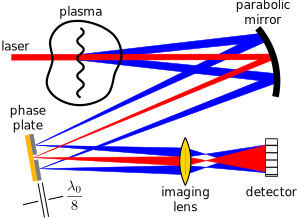
\includegraphics[width = 0.75 \textwidth]{%
    Chapters/InterferometricMethods/figs/pci_schematic.pdf}
  \caption[Schematic overview of a typical PCI system]{%
    Schematic overview of a typical PCI system.
    A plasma-density fluctuation weakly scatters an incident probe beam, and
    an off-axis parabolic mirror focuses the scattered and unscattered beams.
    An optical element known as a phase plate
    is placed at the focal plane of the parabolic mirror.
    The phase plate has a narrow groove of depth $\lambda_0 / 8$
    that imparts phase delay $\pi / 2$ to the unscattered beam,
    effectively converting the unscattered beam
    into an ``internal'' reference beam
    against which the scattered beams can be interfered.
    A lens, whose object plane sits at the plasma midplane,
    is then used to image the resulting radiation onto a detector array.}
  \label{fig:InterferometricMethods:pci_schematic}
\end{figure}


\subsection{Reference-beam generation with a phase plate}
PCI uses an optical element known as a \emph{phase plate}
to delay the unscattered beam by $\pi / 2$
relative to the scattered beams.
The phase plate is typically a reflective optical element
with a groove that is precisely fabricated
to have a depth of $\lambda_0 / 8$;
the unscattered beam reflects off of this groove, and
the corresponding $\lambda_0 / 4$-increase in path length
phase delays the unscattered beam by $\pi / 2$
relative to the scattered beams,
which reflect off of the non-grooved portions
(i.e.\ the ``face'') of the phase plate.
To boost the relative size of the fluctuating signal,
the phase groove typically reflects only a fraction $\eta < 1$
of the incident unscattered beam power, while
the phase-plate face reflects all of the scattered beam power.
Thus, by the action of the phase plate,
$1 \rightarrow i \sqrt{\eta}$ in the imaged electric field
(\ref{eq:InterferometricMethods:imaged_total_field_monochromatic_fluctuation_weak_coupling})
such that
\begin{equation}
  E_{\text{PCI}}(\vect{r}_{\image}, t)
  =
  i E_G(\vect{r}_{\image}, t) e^{i \bar{\phi}}
  \left[%
    \sqrt{\eta} + \tilde{\phi}_0 \cos\nu
  \right],
  \label{eq:InterferometricMethods:pci_imaged_field}
\end{equation}
and the corresponding intensity,
averaged over an optical cycle and
to first order in $\tilde{\phi}_0$, is
\begin{equation}
  I_{\text{PCI}}(\vect{r}_{\image}, t)
  =
  I_G(\vect{r}_{\image})
  \left[%
    \eta
    +
    2 \sqrt{\eta} \tilde{\phi}_0 \cos\nu
  \right].
  \label{eq:InterferometricMethods:pci_intensity}
\end{equation}
Here, $E_G(\vect{r}_{\image})$ and $I_G(\vect{r}_{\image})$
are the field and intensity profiles
of the unscattered Gaussian beam on the detector
in the \emph{absence} of the phase plate,
with $I_G(\vect{r}_{\image})$ being explicitly defined in
(\ref{eq:InterferometricMethods:Gaussian_beam_intensity}).
Equation
(\ref{eq:InterferometricMethods:pci_intensity})
should be contrasted with
(\ref{eq:InterferometricMethods:imaged_field_intensity}),
which gives the image-plane intensity
in the absence of the phase plate.
Thus, the phase plate converts the unscattered probe beam
into an effective reference beam for the scattered beams.


\subsection{Focal-plane separation of scattered beams}
Implicit in the use of the phase plate
is that the scattered and unscattered beams
are well-separated in space
such that the phase groove only affects the unscattered beam.
The 1\ts{st}-order scattered beams are angularly separated
from the unscattered beam by $\theta = k / k_0$, and,
in the far field ($z \gg z_R$),
the center of the scattered beam will fall outside of
the unscattered beam's 1/e $E$ radius if
\begin{equation}
  |k| \geq \frac{2}{w_0}.
  \label{eq:InterferometricMethods:kmin_for_far_field_beam_separation}
\end{equation}
However, CO$_2$ laser beams used to probe tokamak plasmas often have
$z_R \gg \SI{10}{\meter}$, so
the beam's far field is not easily accessible in typical lab settings.
Fortunately, the far-field diffraction pattern
can be equivalently accessed in the focal plane
of a focusing optic~\cite[Ch.~8]{born_and_wolf}.

The focal-plane location, beam size, and beam separation
can be easily determined.
Let the Gaussian probe beam have
an in-vessel 1/e $E$ waist radius of $w_0$,
and place a focusing optic of focal length $f$
a distance $s$ downstream from the in-vessel beam waist.
Then, the waist of the focused beam
will be located a distance $s'$ downstream of the focusing optic
and will have 1/e $E$ radius $w_0'$ given as
\begin{align}
  s' &= f \left( 1 + \frac{s - f}{z_R} \right),
  \\
  w_0' &= \frac{w_0 |f|}{\left[ (s - f)^2 + z_R^2 \right]^{1/2}},
\end{align}
where $z_R$ is the in-vessel Rayleigh length~\cite{self83}.
When $|s - f| \ll z_R$, as is typical for PCI,
the expressions for $s'$ and $w_0'$ reduce to
\begin{align}
  s' &\approx f,
  \label{eq:InterferometricMethods:focal_plane_location_rayleigh}
  \\
  w_0' &\approx \frac{2 |f|}{k_0 w_0}.
  \label{eq:InterferometricMethods:focal_plane_waist_rayleigh}
\end{align}
The spatial separation $\Delta$
of the scattered and unscattered beams in the focal plane
is found by applying the appropriate $ABCD$ ray matrices
from Table~\ref{table:ImagingSystems:ABCD_matrices}
to a ray scattered in the plasma midplane by angle $\theta$, i.e.\
\begin{align}
  \begin{pmatrix}
    \Delta
    \\
    \theta_{pp}
  \end{pmatrix}
  &=
  \begin{pmatrix}
    1 & s'
    \\
    0 & 1
  \end{pmatrix}
  \begin{pmatrix}
    1      & 0
    \\
    -1 / f & 1
  \end{pmatrix}
  \begin{pmatrix}
    1 & s
    \\
    0 & 1
  \end{pmatrix}
  \begin{pmatrix}
    0
    \\
    \theta
  \end{pmatrix},
  \notag
\end{align}
which, upon substitution of
of the focal plane location from
(\ref{eq:InterferometricMethods:focal_plane_location_rayleigh}) and
the scattering angle $\theta = k / k_0$,
simplifies to
\begin{equation}
  \Delta
  \approx
  \frac{k f}{k_0}.
  \label{eq:InterferometricMethods:phase_plate_beam_separation}
\end{equation}


\subsection{Low-$k$ cutoff of phase plate}
Now, let the phase-plate groove have a width $d$, as is shown in
Figure~\ref{fig:InterferometricMethods:phase_plate_beam_separation}.
Finite PCI response requires that (most of) the scattered beams
fall outside of the phase groove (i.e.\ $|\Delta| \geq d / 2$).
Application of the phase-plate beam-separation formula
(\ref{eq:InterferometricMethods:phase_plate_beam_separation})
then shows that there will be finite PCI response
for $|k| \geq k_g$, where
\begin{equation}
  k_g \equiv \frac{k_0 d}{2 f}.
  \label{eq:InterferometricMethods:pci_kmin_engineering}
\end{equation}
Here, the subscript $g$ is in reference
to the \emph{groove} of the phase plate.
Further, to provide the strongest phase contrast,
the unscattered beam should fall wholly within the phase groove
(i.e.\ $2 w_0' \leq d$);
substituting (\ref{eq:InterferometricMethods:focal_plane_waist_rayleigh})
for $w_0'$ then yields a constraint on the phase groove width
\begin{equation}
  d \geq \frac{4 f}{k_0 w_0},
  \label{eq:InterferometricMethods:phase_groove_constraint}
\end{equation}
and inserting (\ref{eq:InterferometricMethods:phase_groove_constraint}) into
(\ref{eq:InterferometricMethods:pci_kmin_engineering}) yields
\begin{equation}
  k_g \geq \frac{2}{w_0}.
  \label{eq:InterferometricMethods:pci_kmin_physics}
\end{equation}
As finite response requires that $|k| \geq k_g$, it follows that
(\ref{eq:InterferometricMethods:pci_kmin_physics}) is equivalent to
(\ref{eq:InterferometricMethods:kmin_for_far_field_beam_separation}),
which was derived by considering the far-field separation
of the scattered and unscattered beams.
Thus, PCI's low-$k$ cutoff
is ultimately constrained by the in-vessel beam size $w_0$,
with diffraction being the constraining physical mechanism.

\begin{figure}
  \centering
  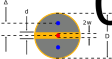
\includegraphics[width = 0.75 \textwidth]{%
    Chapters/InterferometricMethods/figs/phase_plate_beam_separation.pdf}
  \caption[Transverse phase-plate dimensions]{%
    Transverse phase-plate dimensions.
    The unscattered beam is shown in red, while
    the scattered beams are shown in blue.}
  \label{fig:InterferometricMethods:phase_plate_beam_separation}
\end{figure}


\subsection{High-$k$ cutoff of phase plate}
Let the phase plate have a diameter $D$, as is shown in
Figure~\ref{fig:InterferometricMethods:phase_plate_beam_separation}.
Detection of the scattered radiation
requires that (most of) the scattered beam reflect
from the face of the phase plate
(e.g.\ $\Delta \leq D / 2$).
Application of the phase-plate beam-separation formula
(\ref{eq:InterferometricMethods:phase_plate_beam_separation})
then shows that there will be finite PCI response for $|k| \leq k_D$ where
\begin{equation}
  k_D \equiv \frac{k_0 D}{2 f}.
  \label{eq:InterferometricMethods:pci_kmax_engineering}
\end{equation}


\subsection{Effect of phase plate on $m$\ts{th} scattered beam}
The effect of the PCI phase plate on the $m$\ts{th} scattered beam
is given by the complex-valued function $\mathcal{E}(\vect{r}_m, k)$,
which is derived and thoroughly discussed in
Appendix~\ref{app:PCIResponseIdentities}.
The relevant results are briefly summarized here for completeness.
Eq.~(\ref{eq:PCIResponseIdentities:transformation_Hermitian_decomposed})
shows that PCI's image-plane $\mathcal{E}(\vect{r}_m, k)$
readily reduces to
\begin{equation}
  \begin{aligned}
    \mathcal{E}(\vect{r}_{m,\image}, k_{\image})
    &=
    e^{-[x_{m,\image} / w(z_{m,\image})]^2}
    e^{i m k_{\image} x_{\image}}
    \\
    &\quad\times
    \left[%
      F(\vect{r}_{m,\image}, k_{\image})
      +
      G(\vect{r}_{m,\image}, k_{\image})
    \right],
  \end{aligned}
  \label{eq:InterferometricMethods:PCI_transformation_Hermitian_decomposed}
\end{equation}
where the phase-plate face acts on the $m$\ts{th} scattered beam via $F$, and
the phase-plate groove acts on the $m$\ts{th} scattered beam via $G$.
$F$ and $G$ are themselves defined in
(\ref{eq:PCIResponseIdentities:transformation_face}) and
(\ref{eq:PCIResponseIdentities:transformation_groove}).
Of particular note, $F$ is Hermitian with respect to $m$
\begin{equation}
  F(\vect{r}_{-m,\image}, k_{\image})
  =
  F^*(\vect{r}_{m,\image}, k_{\image}),
  \label{eq:InterferometricMethods:mth_beam_interaction_with_face_hermitian}
\end{equation}
while $G$ is anti-Hermitian with respect to $m$
\begin{equation}
  G(\vect{r}_{-m,\image}, k_{\image})
  =
  -G^*(\vect{r}_{m,\image}, k_{\image}).
  \label{eq:InterferometricMethods:mth_beam_interaction_with_groove_antihermitian}
\end{equation}
These symmetries imply
that $F(\vect{r}_{0,\image}, k_{\image})$ is purely \emph{real} and
that $G(\vect{r}_{0,\image}, k_{\image})$ is purely \emph{imaginary}.


\subsection{The imaged field and its intensity}
\label{sec:InterferometricMethods:pci:imaged_field_and_intensity}
Introducing the notational shorthand
$F_m \equiv F(\vect{r}_{m,\image}, k_{\image})$ and
$G_m \equiv G(\vect{r}_{m,\image}, k_{\image})$,
the weak-coupling ($\tilde{\phi}_0 \ll 1$), image-plane electric field from
(\ref{eq:InterferometricMethods:imaged_total_field_weak_coupling_Fourier_filtered})
readily reduces to
\begin{equation}
  \begin{aligned}
  E(\vect{r}_{\image}, t)
  \approx
  E_G(\vect{r}_{\image}, t)
  e^{i \bar{\phi}}
  \biggl\{%
    F_{0} + G_{0}
    &+
    i \frac{\tilde{\phi}_0}{2}
    \biggl[
      (F_{1} + G_{1}) e^{i \nu}
      \\
      &+
      (F_{-1} + G_{-1}) e^{-i \nu}
    \biggr]
  \biggr\},
  \end{aligned}
\end{equation}
where the approximation $w(z_m) \approx w(z)$ has been used,
$\nu$ is defined in (\ref{eq:InterferometricMethods:image_plane_nu}), and
$E_G(\vect{r}_{\image}, t)$ would be the image-plane electric field
of the unscattered beam in the \emph{absence} of the phase plate.
Now, recall that $F$ is Hermitian such that
$F_{-1} = F^{*}_{1}$ and $F_{0} = \real(F_{0})$ and
that $G$ is anti-Hermitian such that
$G_{-1} = -G^{*}_{1}$ and $G_{0} = {i \cdot \imag(G_{0})}$;
using these substitutions, the field further reduces to
\begin{equation}
  \begin{aligned}
    E(\vect{r}_{\image}, t)
    =
    E_G(\vect{r}_{\image}, t)
    e^{i \bar{\phi}}
    \biggl\{%
      &\real(F_0) - \tilde{\phi}_0 \imag(G_1 e^{i \nu})
      \\
      &+
      i \left[ \imag(G_0) + \tilde{\phi}_0 \real(F_1 e^{i \nu}) \right]
    \biggr\},
  \end{aligned}
\end{equation}
and the corresponding intensity,
averaged over an optical cycle and
to first order in $\tilde{\phi}_0$, is
\begin{equation}
  \begin{aligned}
    I_{\text{pci}}(\vect{r}_{\image}, t)
    &=
    I_G(\vect{r}_{\image})
    \biggl\{%
      |F_0|^2 + |G_0|^2
      \\
      &
      +
      2 \tilde{\phi}_0
      \bigl[%
        \imag(G_0) \real(F_1 e^{i \nu})
        -
        \real(F_0) \imag(G_1 e^{i \nu})
      \bigr]
    \biggr\},
  \end{aligned}
\end{equation}
where $I_G(\vect{r}_{\image})$
would be the intensity profile (averaged over an optical cycle)
of the unscattered beam in the \emph{absence} of the phase plate.
Using the fact that $e^{i \nu} = \cos\nu + {i \sin\nu}$,
$F_1 = \real(F_1) + {i \cdot \imag(F_1)}$, and
$G_1 = \real(G_1) + {i \cdot \imag(G_1)}$,
the image-plane intensity further reduces to
\begin{equation}
  \begin{aligned}
    I_{\text{pci}}(\vect{r}_{\image}, t)
    &=
    I_G(\vect{r}_{\image})
    \biggl\{%
      |F_0|^2 + |G_0|^2
      \\
      &+
      2 \tilde{\phi}_0
      \left[ \imag(G_0)\real(F_1) - \real(F_0)\imag(G_1) \right] \cos\nu
      \\
      &-
      2 \tilde{\phi}_0
      \left[ \imag(G_0)\imag(F_1) + \real(F_0)\real(G_1) \right] \sin\nu
    \biggr\}.
  \end{aligned}
  \label{eq:InterferometricMethods:PCI_image_plane_intensity_linear_combination_of_sine_and_cosine}
\end{equation}

Note that the linear combination
$A_I \cos \nu - A_Q \sin \nu$ for real $A_I$, $A_Q$, and $\nu$
can be rewritten as
\begin{align}
  A_I \cos \nu - A_Q \sin \nu
  &=
  A \cos(\nu + \theta),
  \label{eq:InterferometricMethods:linear_combination_of_sine_and_cosine}
\end{align}
where
$A = (A_I^2 + A_Q^2)^{1/2}$,
$\theta = \atantwo(A_Q, A_I)$,
and $\atantwo(A_Q, A_I)$ is the arctangent function of two arguments, which
uses the signs of $A_Q$ and $A_I$ to correctly determine the quadrant
corresponding to a tangent of $A_Q / A_I$.
Note that the notation is mnemonic:
$A_I$ is the amplitude of the ``in-phase'' ($I$) component
(i.e.\ proportional to the image of the assumed
cosine phase fluctuation $\tilde{\phi}(x, t)$ from
(\ref{eq:InterferometricMethods:cosine_phase_fluctuation})), and
$A_Q$ is the amplitude of the corresponding ``quadrature'' ($Q$) component.

As was the case for external reference-beam interferometry,
it is useful to characterize PCI's performance
relative to the saturation limits of a given detector.
Because $\tilde{\phi}_0 \ll 1$,
the PCI optical intensity
(\ref{eq:InterferometricMethods:PCI_image_plane_intensity_linear_combination_of_sine_and_cosine})
satisfies
\begin{align}
  I_{\text{pci}}(\vect{r}_{\image}, t)
  &\lesssim
  I_G(0)
  \left( |F_0|^2 + |G_0|^2 \right),
  \notag
\end{align}
where $I_G(0) = I_G(\rho_{\image} = 0, z_{\image})$ is convenient shorthand
for the peak intensity of the unscattered Gaussian probe beam at the detector
in the \emph{absence} of the phase plate.
To obtain optimal performance, select $I_G(0)$ such that
\begin{equation}
  I_{\text{sat}}
  =
  I_G(0)
  \left( |F_0|^2 + |G_0|^2 \right),
  \notag
\end{equation}
where $I_{\text{sat}}$ is the detector's linear saturation intensity.
Then, taking inspiration from
(\ref{eq:InterferometricMethods:linear_combination_of_sine_and_cosine}),
the image-plane PCI intensity fluctuations from
(\ref{eq:InterferometricMethods:PCI_image_plane_intensity_linear_combination_of_sine_and_cosine})
can be rewritten as
\begin{equation}
  \frac{\tilde{I}_{\text{pci}}(\vect{r}_{\image}, t)}{I_{\text{sat}}}
  =
  \frac{I_G(\vect{r}_{\image})}{I_G(0)}
  \cdot
  A_{\text{pci}}(k_{\image}, x_{\image})
  \cdot
  \tilde{\phi}_0
  \cos\left[ \nu + \theta_{\text{pci}}(k_{\image}, x_{\image}) \right],
\end{equation}
where
\begin{align}
  A_{\text{pci}}(k_{\image}, x_{\image})
  &\equiv
  \frac{2 A(k_{\image}, x_{\image})}{|F_0|^2 + |G_0|^2},
  \label{eq:InterferometricMethods:PCI_amplitude_response}
  \\
  \theta_{\text{pci}}(k_{\image}, x_{\image})
  &\equiv
  \atantwo(A_Q, A_I),
\end{align}
and
\begin{align}
  A(k_{\image}, x_{\image})
  &\equiv
  (A_I^2 + A_Q^2)^{1/2},
  \\
  A_I(k_{\image}, x_{\image})
  &\equiv
  \imag(G_0)\real(F_1) - \real(F_0)\imag(G_1),
  \label{eq:InterferometricMethods:PCI_response_AI}
  \\
  A_Q(k_{\image}, x_{\image})
  &\equiv
  \imag(G_0)\imag(F_1) + \real(F_0)\real(G_1).
  \label{eq:InterferometricMethods:PCI_response_AQ}
\end{align}

Thus, the action of the phase plate results in both
an amplitude response $A_{\text{pci}}(k_{\image}, x_{\image})$ and
a phase response $\theta_{\text{pci}}(k_{\image}, x_{\image})$
in PCI's image-plane intensity.
The on-axis responses $A_{\text{pci}}(k_{\image}, x_{\image} = 0)$ and
$\theta_{\text{pci}}(k_{\image}, x_{\image} = 0) = 0$
are consistent with previous derivations at $x_{\image} = 0$,
such as \cite[Eq.~2.141]{coda_phd} and \cite[Eq.~20]{rost_low_k_pci}.
The present work, however, explicitly accounts for
the spatial variation in the amplitude and phase responses
across the face of the detector.
Note that PCI operates as a nonlinear system
if there are substantial spatial variations in either
$A_{\text{pci}}$ or $\theta_{\text{pci}}$.
The amplitude and phase responses
can be easily evaluated numerically, and
the results for typical system parameters are shown in
Figure~\ref{fig:InterferometricMethods:phase_plate_amplitude_and_phase_response}.
As is colloquially understood, the amplitude response $A_{\text{pci}}$
drops precipitously for $|k| \lesssim k_g$.
(Additionally, the spatial variation in the amplitude response is minimal).
However, perhaps less well known, is the fact that
the phase response $\theta_{\text{pci}}$ exhibits
dramatic spatial variation for $|k| \lesssim k_g$.
This spatial variation biases the PCI-measured wavenumber $k_{\text{meas}}$
away from the true wavenumber $k$,
as shown in Figure~\ref{fig:InterferometricMethods:pci_wavenumber_upshift}.
The physical explanation for this effect is relatively simple:
a Gaussian beam can be decomposed into a set of infinite plane waves
with a finite spread in transverse wavevectors
(see Section~\ref{sec:InterferometricMethods:Gaussian_beam_diffraction:Gaussian_beam_definition}),
and only the components of the scattered beam
with transverse lab-frame wavenumbers $|k| \geq k_g$
are reflected from the phase-plate face and
produce measurable interference on the PCI detector.

\begin{figure}
  \centering
  \includegraphics[width = \textwidth]{%
    Chapters/InterferometricMethods/figs/pci_amplitude_and_phase_response.pdf}
    \caption[PCI amplitude and phase responses in object-plane coordinates
    ]{%
    PCI amplitude response $A_{\text{pci}}(k, x)$ and
    phase response $\theta_{\text{pci}}(k, x)$
    in object-plane coordinates.
    Spatial coordinates $x$ and wavenumbers $k$ are normalized
    to the 1/e $E$ radius of the in-vessel probe beam, $w_0$.
    The system magnification is $M = 0.5$, a fairly typical value.
    The dashed horizontal lines indicate
    the low-$k$ cutoff of the PCI phase-plate groove, $k_g$;
    here, $k_g = 2 / w_0$,
    which is the minimum value allowed by diffraction,
    as discussed in
    (\ref{eq:InterferometricMethods:pci_kmin_physics}).
    The phase-plate high-$k$ cutoff, $k_D$,
    is taken to be infinite.
    The reflectivity of the phase groove is $\eta = 0.17$,
    which is characteristic of the ZnSe typically
    employed in $\SI{10.6}{\micro\meter}$ optics.
    Note that the low-$k$ phase response $\theta_{\text{pci}}$
    exhibits dramatic spatial variation,
    which results in nonlinear PCI operation for $|k| \lesssim k_g$.
  }
\label{fig:InterferometricMethods:phase_plate_amplitude_and_phase_response}
\end{figure}

\begin{figure}
  \centering
  \includegraphics[width = \textwidth]{%
    Chapters/InterferometricMethods/figs/pci_wavenumber_upshift.pdf}
    \caption[Nonlinear upshift in low-$k$, PCI-measured wavenumber]{%
    PCI-measured wavenumber $k_{\text{meas}}$ vs.\ true wavenumber $k$.
    Wavenumbers are normalized
    to the 1/e $E$ radius of the in-vessel probe beam, $w_0$.
    The system magnification is $M = 0.5$, a fairly typical value.
    The dashed vertical lines indicate
    the low-$k$ cutoff of the PCI phase-plate groove, $k_g$;
    here, $k_g = 2 / w_0$,
    which is the minimum value allowed by diffraction,
    as discussed in
    (\ref{eq:InterferometricMethods:pci_kmin_physics}).
    For $|k| \gtrsim k_g$,
    $k_{\text{meas}}$ has a $1:1$ linear relationship with $k$;
    however, for $|k| \lesssim k_g$,
    $k_{\text{meas}}$ is \emph{not} linearly related to $k$.
    Thus, a transfer-function description of the PCI operation
    is only appropriate for wavenumbers above the low-$k$ cutoff
    ($|k| \gtrsim k_g$).
  }
\label{fig:InterferometricMethods:pci_wavenumber_upshift}
\end{figure}

Thus, for $|k| \lesssim k_g$, PCI operates as a nonlinear system
that cannot be described via a transfer function.
Practically speaking, PCI's nonlinear low-$k$ operation
prevents it from measuring the wavenumbers of low-$k$ fluctuations,
such as MHD and some ion-scale instabilities.
(Of course, because the PCI amplitude response $A_{\text{pci}}$
drops precipitously for $|k| \lesssim k_g$,
such low-$k$ fluctuations may be altogether invisible to PCI anyways).
For $|k| \gtrsim k_g$, however, a transfer function can be defined.
Specifically, for $|k| \gtrsim k_g$,
the phase-plate face reflects the scattered beam
($F_1 \rightarrow 1$), while
the phase-plate groove minimally affects the scattered beam
($G_1 \rightarrow 0$).
Further, assuming the majority of the unscattered beam
falls within the phase groove
(i.e.\ constraint (\ref{eq:InterferometricMethods:phase_groove_constraint})),
the phase-plate groove attenuates and phase shifts the unscattered beam
($G_0 \rightarrow i \sqrt{\eta}$), while
the phase-plate face minimally affects the unscattered beam
($F_0 \rightarrow 0$).
Thus, $\theta_{\text{pci}} \rightarrow 0$ and
$A_{\text{pci}} \rightarrow 2 / \sqrt{\eta}$ such that
the PCI transfer function can be defined as
\begin{equation}
  T_{\text{pci}}(k)
  =
  \begin{cases}
    \dfrac{2}{\sqrt{\eta}}, & |k| \gtrsim k_g \\
    \text{undefined},      & \text{otherwise}
  \end{cases}.
  \label{eq:InterferometricMethods:PCI_wavenumber_transfer_function}
\end{equation}
As presented here, for $|k| \gtrsim k_g$,
$T_{\text{pci}}$ is independent of the fluctuation wavenumber;
however, the finite sampling-volume effects
that accompany any real-world measurement
introduce a wavenumber dependence,
as discussed in
Section~\ref{sec:DesignConsiderations:geometric:finite_sampling_volume}.

As is the case with the homodyne interferometer,
the PCI technique does \emph{not} make an absolute measurement
of the phase-fluctuation amplitude $\tilde{\phi}_0$.
To see this, note that the PCI amplitude response $A_{\text{pci}}$
depends very sensitively on the system alignment,
with slight excursions of the unscattered beam
from the partially reflective phase-plate groove
onto the fully reflective phase-plate face
resulting in macroscopic changes to the power reaching the detector.
Further, power fluctuations at the beam source
can alter $I_G(\vect{r}_{\image})$.
Thus, there are three potentially dynamic quantities:
$\{\tilde{\phi}_0, I_G(\vect{r}_{\image}), A_{\text{pci}}\}$,
but there are only two potentially measurable quantities:
the equilibrium and fluctuating powers.
PCI systems on large, vibration-prone fusion devices
typically employ feedback stabilization
(see e.g.~\cite[Ch.~3.5]{coda_phd})
in order to dynamically maintain
the unscattered beam's alignment
on the phase-plate groove,
minimizing vibrational contamination of the PCI signal.
It is then possible, after measuring a calibration constant,
to \emph{estimate} the phase-fluctuation amplitude $\tilde{\phi}_0$ with PCI.


\section{Selecting an interferometric technique}
\label{sec:InterferometricMethods:selection}
Sections~\ref{sec:InterferometricMethods:interferometry}
and~\ref{sec:InterferometricMethods:pci}
detail external reference-beam interferometry and
phase contrast imaging (PCI), respectively.
The intent of this section is to synthesize these results and
to discuss the strengths and limitations
of these interferometric techniques
so that a suitable method can be selected for a given application.


\subsection{Sensitivity}
\label{sec:InterferometricMethods:selection:sensitivity}
The transfer functions in
Sections~\ref{sec:InterferometricMethods:interferometry}
and~\ref{sec:InterferometricMethods:pci}
specify the fraction of a given detector's dynamic range
that is occupied by the fluctuating signal.
If identical detectors are used for each interferometric method,
then an ``apples-to-apples'' comparison of fluctuation sensitivities
can be made by examining the amplitudes
of the corresponding transfer functions.
(See Section~\ref{sec:InterferometricMethods:selection:temporal_bandwidth}
for practical considerations regarding detector selection).
Just such a comparison is shown in
Figure~\ref{fig:InterferometricMethods:interferometric_method_transfer_functions}.
Clearly, for a given fluctuation ($|k| \gtrsim k_g$) and a given detector,
PCI has the best sensitivity.
Specifically, PCI is
$T_{\text{pci}} / T_{\text{hom}} = 2 / \sqrt{\eta}$
more sensitive than a comparable homodyne interferometer
($\phi_R - \bar{\phi} = \pi / 2$) and
$T_{\text{pci}} / T_{\text{het}} = 2 \pi \sqrt{2 / \eta}$
more sensitive than a comparable heterodyne interferometer.
Relative to homodyne interferometry,
PCI's enhanced sensitivity is wholly attributable
to the partial reflectivity ($\eta < 1$) of the phase-plate groove:
the decreased power in the unscattered beam
increases the fraction of the detector's dynamic range
occupied by the fluctuating signal.
The sensitivity deficit of heterodyne interferometry
relative to homodyne interferometry
has two physical origins:
first, the heterodyne interferometer
must capture the full sinusoidal waveform
of the heterodyne interference signal,
which mandates reduction of the mean optical intensity
(and, correspondingly, the fluctuating optical intensity)
at the detector by a factor of two
relative to that of the homodyne interferometer;
second, demodulation of the heterodyne interference signal
additionally attenuates the fluctuating signal.

\begin{figure}
  \centering
  \includegraphics[width = \textwidth]{%
    Chapters/InterferometricMethods/figs/interferometric_method_comparison.pdf}
  \caption[Comparison of interferometric-method transfer functions]{%
    A comparison of the transfer functions for
    PCI
    (\ref{eq:InterferometricMethods:PCI_wavenumber_transfer_function}),
    heterodyne interferometry
    (\ref{eq:InterferometricMethods:heterodyne_interferometer_wavenumber_transfer_function}),
    and homodyne interferometry
    (\ref{eq:InterferometricMethods:homodyne_interferometer_wavenumber_transfer_function},
    in the optimal fluctuation configuration
    with $\phi_R - \bar{\phi} = \pi / 2$).
    Object-plane wavenumbers $k$ are normalized
    to the 1/e $E$ radius of the in-vessel probe beam, $w_0$.
    The magnification of each system is taken to be $|M| = 0.5$,
    which is a representative ``typical'' value.
    The vertical, dashed lines indicate
    the low-$k$ cutoff of the PCI phase-plate groove, $k_g$;
    here, $k_g = 2 / w_0$,
    which is the minimum value allowed by diffraction,
    as discussed in
    (\ref{eq:InterferometricMethods:pci_kmin_physics}).
    The phase-plate high-$k$ cutoff, $k_D$,
    is taken to be infinite.
    The reflectivity of the PCI phase groove is $\eta = 0.17$,
    which is characteristic of the ZnSe typically
    employed in $\SI{10.6}{\micro\meter}$ optics.
    Because the PCI transfer function is not defined for $|k| \lesssim k_g$,
    the low-$k$ PCI amplitude response
    (\ref{eq:InterferometricMethods:PCI_amplitude_response})
    is indicated by the dash-dot curves instead.
  }
\label{fig:InterferometricMethods:interferometric_method_transfer_functions}
\end{figure}

The enhanced sensitivity of PCI and homodyne interferometry
relative to that of heterodyne interferometry
comes with several costs, however.
First, as previously discussed,
neither PCI nor homodyne interferometry
measure the absolute scale of phase fluctuations, while
heterodyne interferometry does.
Second, PCI depends sensitively on the position
of the unscattered beam relative to the phase-plate groove, and
homodyne interferometry depends sensitively on $\phi_R - \bar{\phi}$;
often, feedback stabilization is required
to dynamically maintain the optimal configuration
\cite[Ch.~3.5]{coda_phd}\cite{nazikian_rsi87}.
While feedback stabilization is an added technical complication,
it should be noted that such feedback
is expected to become more commonplace
for laser diagnostics on large fusion devices,
such as ITER's heterodyne interferometer
\cite{vanzeeland_TIP_rsi13}.
Finally, PCI cannot measure the equilibrium phase $\bar{\phi}$.
This makes intuitive sense:
$\bar{\phi}$ uniformly affects both the scattered and unscattered beams,
the PCI phase delays the unscattered beam
to generate an ``internal'' reference beam, and
the $\bar{\phi}$ information cancels in the resulting interference.
A homodyne interferometer operated with $\phi_R - \bar{\phi} = \pi / 2$
is similarly unable to measure $\bar{\phi}$.
In contrast, a heterodyne interferometer
can always measure both the equilibrium phase $\bar{\phi}$ and
the fluctuating phase $\tilde{\phi}$.


\subsection{Spatial bandwidth}
PCI's sensitivity comes at the additional expense of spatial bandwidth.
Specifically, the creation of an ``internal'' reference beam
via spatial filtering
produces a low-$k$ cutoff in the PCI response, as shown in
Figure~\ref{fig:InterferometricMethods:interferometric_method_transfer_functions}.
The minimum size of this cutoff is
set by diffraction of the in-vessel probe beam
(\ref{eq:InterferometricMethods:pci_kmin_physics}), but
it is not uncommon for the realized cutoff
(\ref{eq:InterferometricMethods:pci_kmin_engineering})
to be $\sim 2-3\times$ larger than the diffraction limit.
As shown in Figures~\ref{fig:InterferometricMethods:phase_plate_amplitude_and_phase_response}
and \ref{fig:InterferometricMethods:pci_wavenumber_upshift},
PCI operates as a nonlinear system below its low-$k$ cutoff,
preventing a transfer-function description of its low-$k$ behavior.
In contrast, by using an external reference beam,
homodyne and heterodyne interferometers
operate as linear systems over the entire wavenumber spectrum and
are even capable of making measurements at $k = 0$.

Now, colloquially, interferometry is considered a ``low-$k$'' technique, and
PCI is considered a ``high-$k$'' technique.
However, as detailed in
Section~\ref{sec:InterferometricMethods:Gaussian_beam_diffraction:from_plasma_density_fluctuations},
for a given probe beam and a given fluctuation $\tilde{\phi}$,
the laser-plasma interaction is \emph{identical}
for both interferometry and PCI.
Further, the high-$k$ optical capabilities of interferometry and PCI
are governed by the size of the collection optics
and finite sampling-volume effects~\cite{bravenec_rsi95}.
Thus, there is nothing that intrinsically limits
interferometry to low-$k$ measurements ---
an interferometer's high-$k$ limit
can be just as high, if not higher,
than that of a given PCI system.
However, as discussed in
Section~\ref{sec:InterferometricMethods:selection:sensitivity},
PCI is \emph{more sensitive} to fluctuations
than a comparable interferometer, and,
assuming a Kolmogorov-like fluctuation spectrum
$S(k) \propto k^{-p}$ for some positive $p$,
PCI's superior sensitivity may allow it
to detect high-$k$ fluctuations
that are too weak to be seen by an interferometer.


\subsection{Temporal bandwidth}
\label{sec:InterferometricMethods:selection:temporal_bandwidth}
Detector bandwidth is often the dominant constraint
of an interferometric system's temporal bandwidth.
Homodyne interferometry and PCI require
\begin{equation}
  \omega_{\text{det}} > \omega,
  \qquad \qquad \quad% \qquad
  \text{homodyne interferometry, PCI,}
\end{equation}
where
$\omega_{\text{det}}$ is the angular cutoff frequency of the detector and
$\omega$ is the angular frequency of the fluctuation.
Heterodyne interferometry, however, requires
\begin{equation}
  \omega_{\text{det}} > \Delta \omega_0 + \omega,
  \qquad
  \text{heterodyne interferometry,}
\end{equation}
where $\Delta \omega_0$ is the (angular) intermediate frequency.
Further, proper reconstruction of the baseband signal
from the heterodyne interference signal requires $\omega < \Delta \omega_0$.

Thus, for a given fluctuation $\omega \ll \Delta \omega_0$,
heterodyne interferometry requires a much faster detector
than homodyne interferometry or PCI\@.
For the HgCdTe detectors typically used at $\SI{10.6}{\micro\meter}$,
cooling the active element of the detector
reduces detector noise and increases the detector response
at the expense of reduced $\omega_{\text{det}}$.
Thus, for low--bandwidth applications ($\omega \ll \Delta \omega_0$),
homodyne interferometry and PCI may be able to use
slower, cooled detectors that are less noisy than
the comparable faster, warmer detectors
required for heterodyne interferometry.
The use of less noisy detectors
may produce sensitivity gains for PCI and homodyne interferometry
relative to heterodyne interferometry.
Although use of a ``slow'' detector prevents measurements
of broadband fluctuations beyond the detector cutoff,
it \emph{is} possible to measure coherent, high-frequency fluctuations
well beyond the detector cutoff ($\omega \gg \omega_{\text{det}}$)
by rapidly modulating the intensity of the probe beam
\cite[Sec.~3.3.1]{tsujii_phd}.


\bibliographystyle{plainurl}
\bibliography{references}

\chapter{Implementation of a combined PCI-interferometer on \diiid}


\section{Optical-diagnostic access on \diiid}
\label{sec:Implementation:d3d_ports}
\diiid \space provides optical access to its plasmas
through a number of ports, as indicated in
Fig.~\ref{fig:Implementation:d3d_port_locations}.
The ports are labeled according to their
toroidal positions and their sightlines, and
an experimentalist should have at least
a rough familiarity with these conventions.
The toroidal location of a port
is given in degrees clockwise from ``machine north''
when viewing the machine from above
(note that machine north does \emph{not} correspond
to geographic or magnetic north).
The angular separation of adjacent toroidal ports is $15^{\circ}$.
Port sightlines can be vertical or radial.
Ports with vertical (V) sightlines
are labeled sequentially in terms of increasing major radius,
with $V1$ having the smallest major radius and
$V3$ having the largest major radius.
Radial ports (R) have sightlines
that are roughly aligned with the plasma's minor radius, and
they are labeled according to their positions
relative to the plasma midplane:
R0 sits at the plasma midplane,
R+1 and R+2 are the first and second ports
\emph{above} the plasma midplane, respectively, and
R-1 and R-2 are the first and second ports
\emph{below} the plasma midplane, respectively.

\begin{figure}
  \centering
  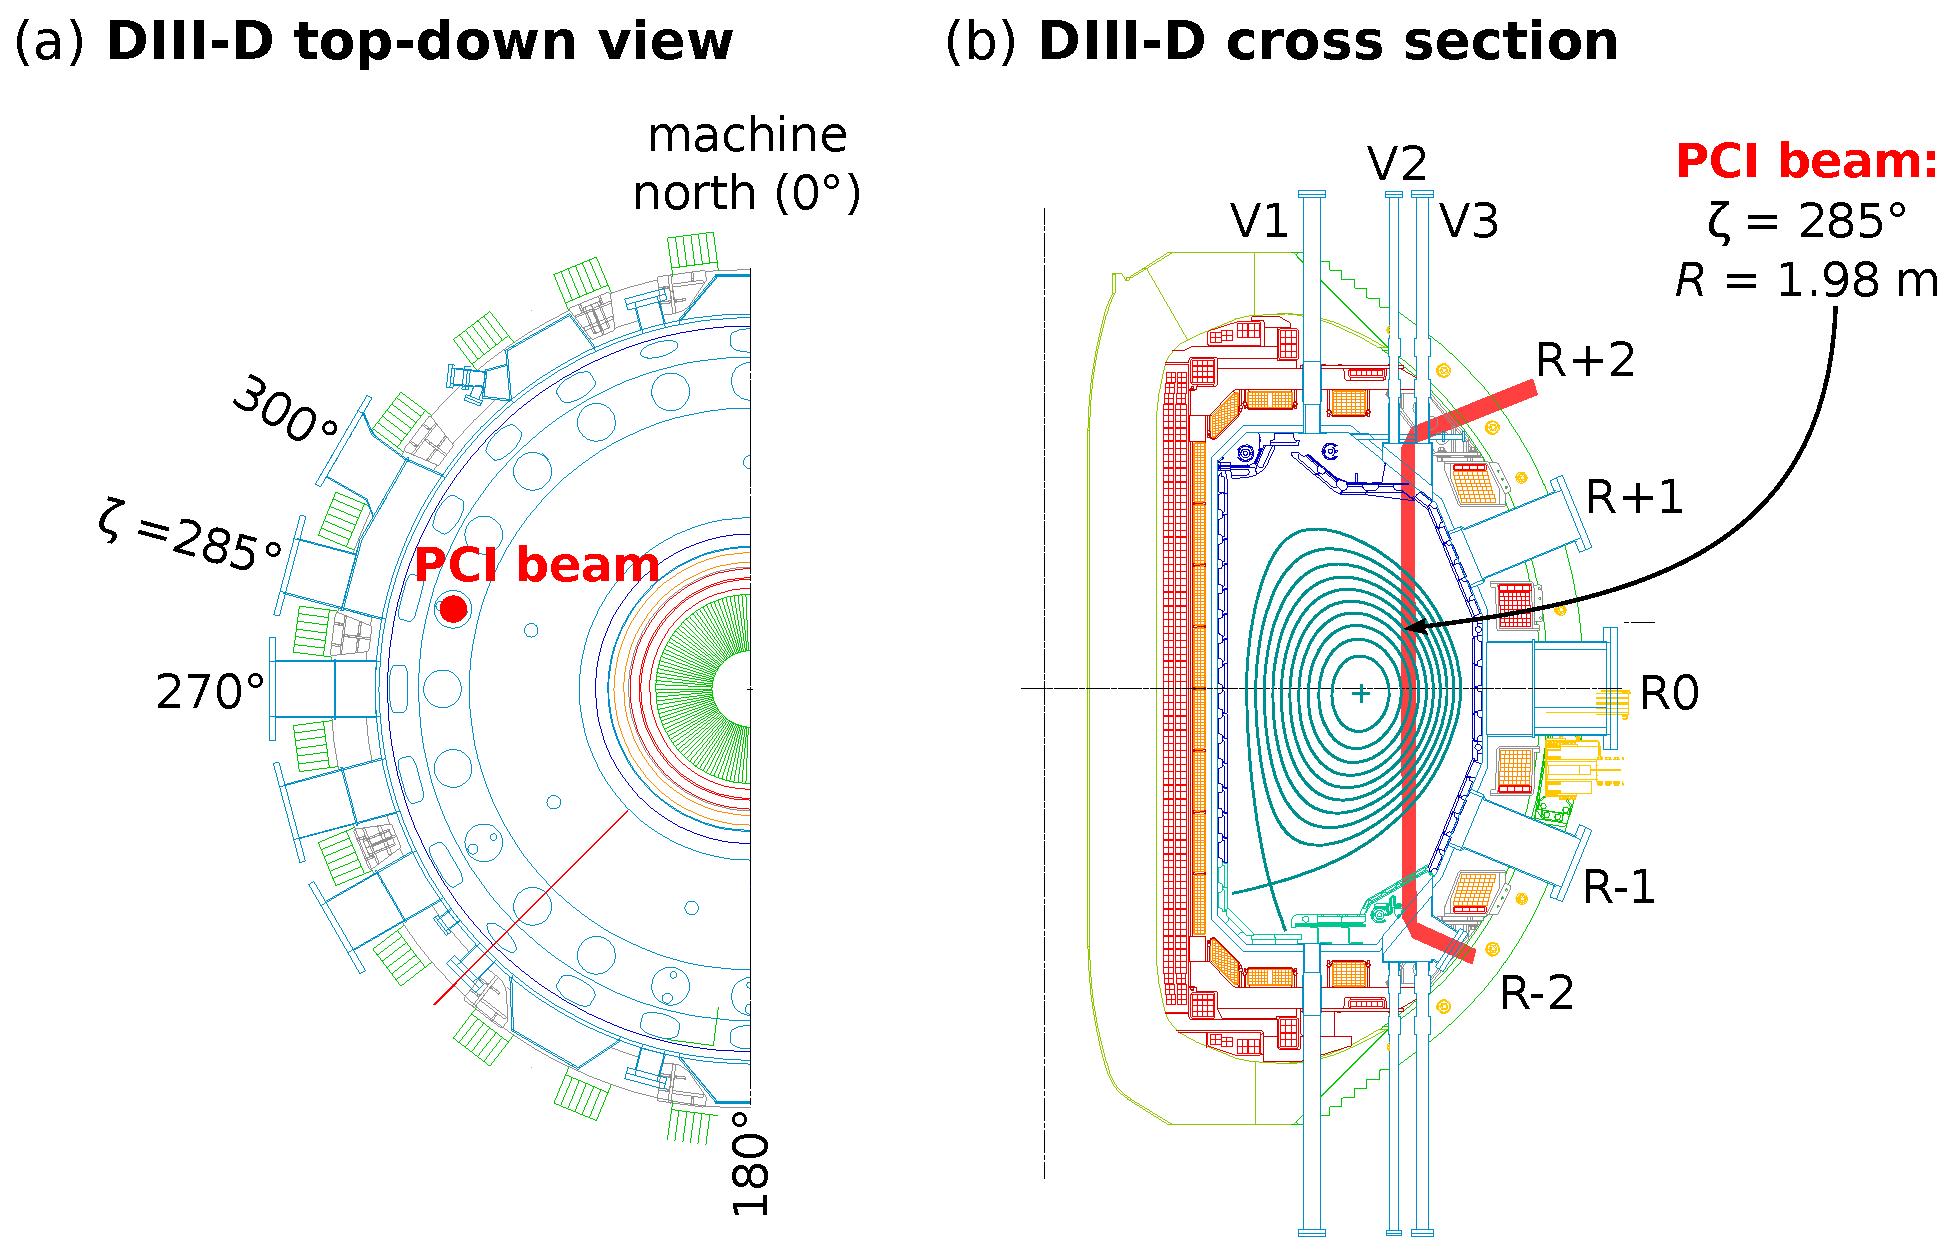
\includegraphics[width = \textwidth]{%
    Chapters/Implementation/figs/d3d_port_locations.pdf}
  \caption[\diiid \space port-labeling conventions and location of PCI]{%
    (a) View of \diiid \space from above,
    indicating the toroidal-labeling convention.
    (b) View of \diiid \space cross section,
    indicating the labeling convention
    for vertical (V) and radial (R) sightlines.
    The PCI beam enters the vessel through the $285^{\circ}$ R+2 port,
    propagates vertically downwards through the plasma
    at a major radius of $R = \SI{1.98}{\meter}$, and
    exits the vessel through the $285^{\circ}$ R-2 port.}
\label{fig:Implementation:d3d_port_locations}
\end{figure}


\section{\diiid's pre-existing PCI system}
The \diiid \space PCI system is
thoroughly described elsewhere~\cite{dorris_rsi09, dorris_phd}, but
the system components of relevance to this work
are briefly summarized below for completeness.


\subsection{System geometry}
The system is currently configured
in the ``Phase II'' geometry~\cite{dorris_rsi09},
with the probe beam propagating vertically downwards
from the $285^{\circ}$ R+2 port to the $285^{\circ}$ R-2 port.
The beam center sits at $R = $ \SI{1.98}{\meter}.
Both the toroidal and radial positions
of the PCI beam are shown in
Fig.~\ref{fig:Implementation:d3d_port_locations}.

The PCI system's vertical beam path constrains
which types of fluctuations it can and cannot detect.
Namely, the PCI-measured power fluctuations
(\ref{eq:InterferometricMethods:PCI_ratio_fluctuating_to_equilibrium_power})
correspond to \emph{line-integrated} electron-density fluctuations, which
are the physical origin of the phase fluctuations $\tilde{\phi}$ in
(\ref{eq:InterferometricMethods:phase_fluctuation}).
Because it is a line-integrated measurement,
only fluctuations propagating perpendicular to the beam path can be detected,
as fluctuations propagating parallel to the beam path
are effectively averaged out of the signal
\graffito{\textcolor{red}{what about $\delta \omega$?}}
(and, at a more fundamental level, fluctuations propagating
parallel to the beam path do \emph{not} spatially scatter the probe beam).
\graffito{\textcolor{red}{citation? Wesson?}}
Now, electrostatic turbulence (e.g.\ ITG, ETG) tends to be field-aligned
such that $k_{\perp} \gg k_{||}$, where
the $\perp$ and $||$ subscripts are used here to indicate
orientations that are perpendicular to and parallel to
the local magnetic field, respectively.
To lowest order, then, electrostatic fluctuations propagate
perpendicular to a tokamak's toroidal field.
PCI's vertical beam path and
the field-aligned constraint of electrostatic turbulence
imply that PCI is predominantly sensitive to fluctuations
with finite major-radial wavenumber $k_R$.
Thus, PCI's 32-element, 1-dimensional detector array
is oriented in the image plane such that
each detector element corresponds to a unique major radius in the plasma.

In some situations, 2-dimensional detector arrays
\cite{sanin_rsi04, tanaka_rsi16} or
spatially filtering ``masks''~\cite{dorris_rsi09, dorris_phd, lin_rsi06}
can be used to localize measurements
by exploiting the spatial variation
in the magnetic field's orientation along the beam path.
These localization techniques typically work best
for high-$k$ measurements.
Note that $k_R$ is related to the
often-theoretically-relevant poloidal wavenumber $k_{\theta}$ via
\begin{equation}
  k_R = k_{\theta} \csc[\alpha(R, z)],
  \label{eq:Implementation:kR_to_ktheta}
\end{equation}
where $\alpha(R, z)$ is the angle
between the beam path and the local flux surface,
as shown schematically in
Fig.~\ref{fig:Implementation:relating_kR_to_ktheta}.
Of course, the fluctuation measurements must be localized,
either via direct measurement
(with 2-dimensional detector arrays or ``masks'')
or via inference from other plasma properties,
before (\ref{eq:Implementation:kR_to_ktheta})
can be inverted to yield $k_{\theta}$
from measured values of $k_R$.

\begin{figure}
  \centering
  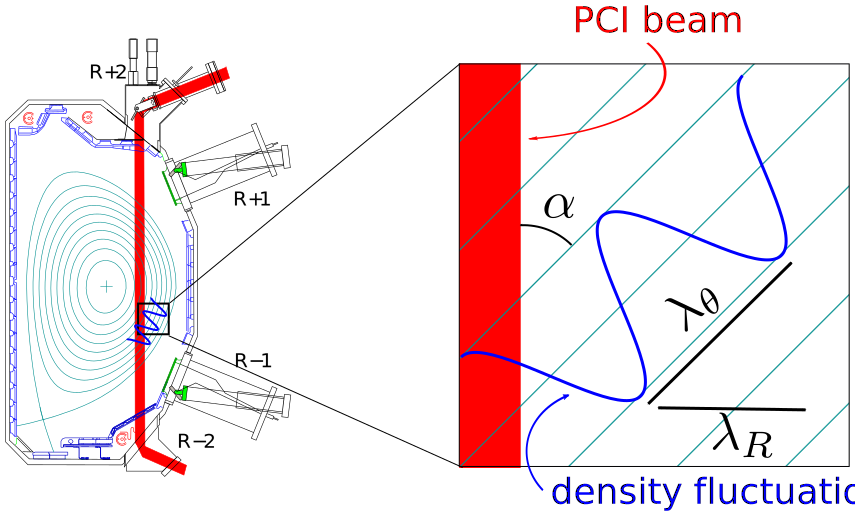
\includegraphics[width = 0.9 \textwidth]{%
    Chapters/Implementation/figs/kR_to_ktheta.pdf}
  \caption[Relating $k_R$ to $k_{\theta}$]{%
    The major-radial wavenumber $k_R = 2 \pi / \lambda_R$ and
    the poloidal wavenumber $k_{\theta} = 2 \pi / \lambda_{\theta}$
    are related via $\alpha(R, z)$, which
    is the angle between PCI's vertical probe beam and
    the local flux surface.}
\label{fig:Implementation:relating_kR_to_ktheta}
\end{figure}


\subsection{Spatial bandwidth}
The system has $k_{\text{min}}^{\text{PCI}} = \SI{1.5}{\per\centi\meter}$.

The 1/e electric field radius of the in-vessel beam is
$w_0 =$ \SI{3.4}{\centi\meter}, and

A pair of fast steering mirrors dynamically centers
the unscattered beam on the phase plate groove,
compensating for vibrations.



\subsection{Temporal bandwidth}


\begin{itemize}
  \item $k$-cutoff
  \item Maintenance
    \begin{itemize}
      \item Replacement of laser
      \item Replacement of feedback detector
      \item Replacement of in-vessel mirrors
    \end{itemize}
\end{itemize}

\section{Interferometer design}
\begin{itemize}
  \item Power sharing between the interferometer arms and PCI
  \item TE-cooled detector
  \item Imaging and $k$-response
  \item Demodulation scheme
\end{itemize}

\section{Interferometer optimization}
\begin{itemize}
  \item LO stability
  \item External clock
\end{itemize}

\section{Sound-wave calibration of combined PCI-interferometer}
\begin{itemize}
  \item Importance of speaker placement
  \item System sensitivity
\end{itemize}


\bibliographystyle{plainurl}
\bibliography{references}

\chapter{Correlation of \diiid's toroidally separated interferometers}
The toroidal structure of an MHD mode can strongly influence
the mode's stability and its interaction with the surrounding plasma.
A mode's toroidal structure is typically characterized
via the toroidal mode number $n$.
Historically, measurement of toroidal (and poloidal) mode numbers
with magnetic loops has provided rich insight
into the physics governing numerous operational regimes and stability limits.
However, core-localized MHD produces weak signals outside of the plasma volume,
making measurement of mode numbers via magnetic loops difficult or impossible.
Recently, measurements from toroidally separated
electron cyclotron emission imaging (ECEI) systems
on the KSTAR tokamak have identified mode numbers of
edge-localized modes~\cite{lee_rsi_2014} and
sawteeth~\cite{choe_nf_2015},
raising the question as to the utility of using more exotic measurements
to probe the structure of core-localized MHD.

This chapter describes the use of toroidally separated interferometers
to measure toroidal mode numbers.
To the author's knowledge, this is the first such implementation in a tokamak.
The addition of the heterodyne interferometer channel
to \diiid's pre-existing phase contrast imaging (PCI) system
enabled this novel measurement.
As shown in Fig.~\ref{fig:ToroidalCorrelation:pci_interf_locs}
the beampaths of the PCI and V2 interferometers
are toroidally separated by $\Delta \zeta = 45^{\circ}$ and
are very nearly radially overlapping.
Section~\ref{sec:ToroidalCorrelation:two_point_correlations}
reviews the mathematics of the two-point-correlation technique
used to extract toroidal mode numbers and
derives the resulting Nyquist mode number.
Section~\ref{sec:ToroidalCorrelation:interferometer_measurements}
examines the interferometer measurements in detail and
develops a formula for the measured toroidal mode number.
Section~\ref{sec:ToroidalCorrelation:nonideal_effects}
characterizes the effects of time-base offsets and radial offsets
between the two interferometer systems and
describes methods to minimize their influence
on the measured toroidal mode number.

\begin{figure}
  \centering
  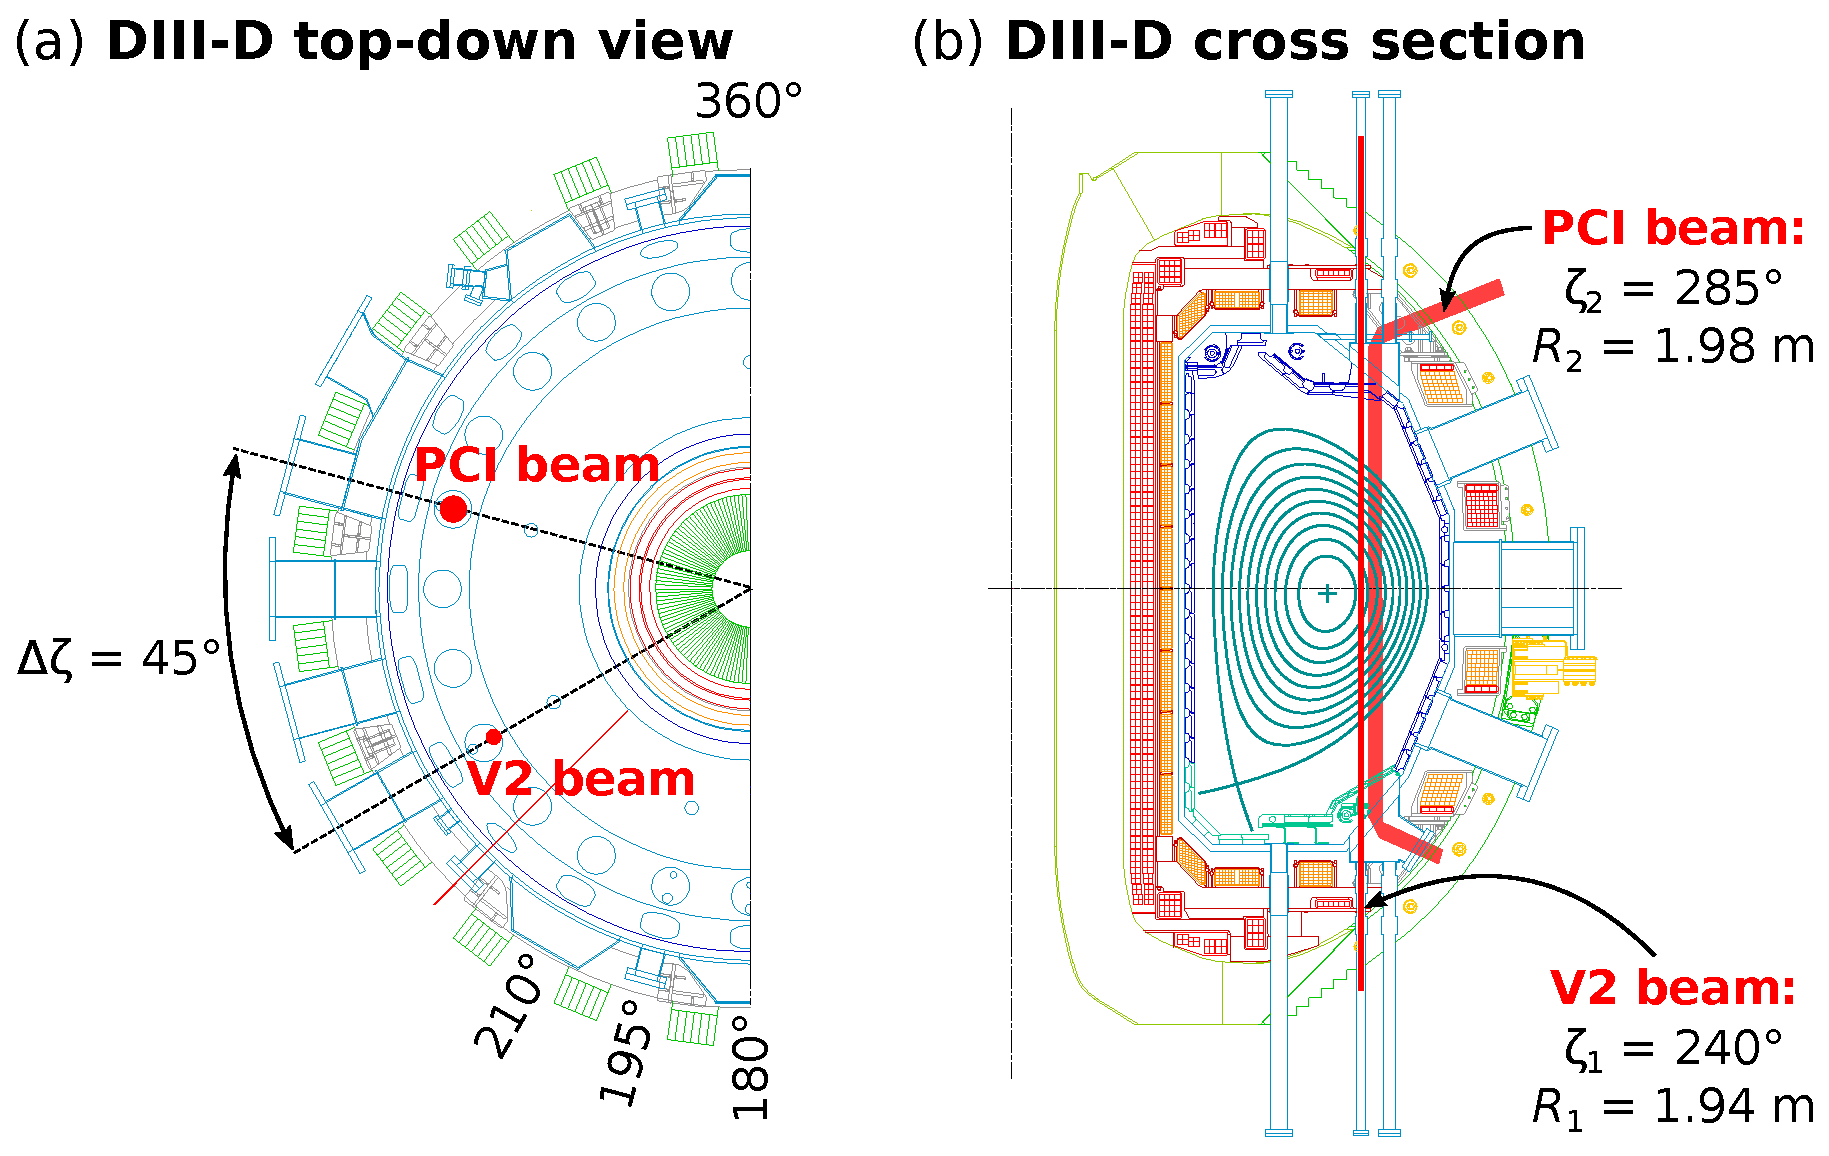
\includegraphics[width = \textwidth]{%
    Chapters/ToroidalCorrelation/figs/pci_interf_locs.eps}
  \caption[Beam locations of the V2 interferometer and PCI systems on \diiid]{%
    (a) A top-down view of the \diiid\space vessel.
    The V2 interferometer beam's toroidal location is $\zeta_1 = 240^{\circ}$,
    and the PCI beam's toroidal location is $\zeta_2 = 285^{\circ}$.
    (b) A view of the \diiid\space cross section.
    The V2 interferometer beam's
    major-radial location is $R_1 = \SI{1.94}{\meter}$, and
    the PCI beam's major-radial location is $R_2 = \SI{1.98}{\meter}$.}
\label{fig:ToroidalCorrelation:pci_interf_locs}
\end{figure}


\section{Two-point correlations}
\label{sec:ToroidalCorrelation:two_point_correlations}


\subsection{Spectral characterization of random processes}
In contrast to deterministic processes,
random processes cannot be modeled via an explicit mathematical relationship.
Rather, random processes are characterized
in terms of probabilities and statistical properties.
Any given observation of a random process represents
only one of many possible observations;
each such observation is referred to as
a ``sample'' or a ``realization'' of the random process
and is denoted as $x_k(t)$.
The random process itself consists of
the ensemble of all of the potential observations
and is denoted as $\{x_k(t)\}$.
Random processes can be stationary or nonstationary.
The statistical properties of a stationary random process
do not vary in time, and
the spectral tools discussed below
were all developed for analysis of stationary random processes.

The \emph{finite} Fourier transform $X_k(f, T)$
of a continuous signal $x_k(t)$ is defined as
\begin{equation}
  X_k(f, T)
  =
  \int_{-T / 2}^{T / 2}
  dt \, x_k(t) e^{-i \, 2 \pi f t}
  \label{eq:ToroidalCorrelation:finite_Fourier_transform}
\end{equation}
Note that $x_k(t)$ need \emph{not} be integrable over the infinite domain,
making the finite Fourier transform a suitable tool for stationary signals,
whose statistical properties (e.g.\ mean, variance, etc.) are
constant and potentially finite in time.

For real-valued, stationary random processes $\{x_k(t)\}$ and $\{y_k(t)\}$,
the one-sided cross-spectral density function $G_{xy}(f)$ is defined as
\begin{equation}
  G_{xy}(f)
  \equiv
  \lim_{T \rightarrow \infty}
  \frac{2}{T} E \left[ X_k^*(f, T) Y_k(f, T) \right]
  \label{eq:ToroidalCorrelation:cross_spectral_density_defn}
\end{equation}
for $0 < f < \infty$;
$G_{xy}(f)$ is not defined for $f < 0$, and
it is reduced by a factor of two relative to
(\ref{eq:ToroidalCorrelation:cross_spectral_density_defn}) at $f = 0$
(the value of $G_{xy}(0)$ is of little relevance to this work).
Note that $E[\cdot]$ is the expectation value operator;
this operator averages over all of the realizations in the ensemble, and
its application ensures that
(\ref{eq:ToroidalCorrelation:cross_spectral_density_defn})
is a statistically consistent definition of the cross-spectral density
(that is, ensemble averaging is needed for $G_{xy}(f)$
to approach the true cross-spectral density as $T \rightarrow \infty$).
In general $G_{xy}(f)$ is a complex-valued function;
this can be explicitly written as
\begin{equation}
  G_{xy}(f) = \left| G_{xy}(f) \right| e^{i \alpha_{xy}(f)}
  \label{eq:ToroidalCorrelation:cross_spectral_density_explicit_complex}
\end{equation}
where $\alpha_{xy}(f)$ is the \emph{phase angle}.
For the special case $\{x_k(t)\} = \{y_k(t)\}$,
$G_{xx}(f)$ is real-valued (i.e.\ $G_{xx}(f) = |G_{xx}(f)|$) and
is referred to as the one-sided autospectral density function.

The degree of correlation between random processes
$\{x_k(t)\}$ and $\{y_k(t)\}$ can be easily quantified
with the corresponding spectral density functions.
In particular, the magnitude-squared coherence function
$\gamma_{xy}^2(f)$ is defined as
\begin{equation}
  \gamma_{xy}^2(f)
  \equiv
  \frac{|G_{xy}(f)|^2}{G_{xx}(f) G_{yy}(f)}
  \label{eq:ToroidalCorrelation:magnitude_squared_coherence_defn}
\end{equation}
and it satisfies
\begin{equation}
  0 \leq \gamma_{xy}^2(f) \leq 1
  \label{eq:ToroidalCorrelation:magnitude_squared_coherence_bounds}
\end{equation}
for $0 \leq f < \infty$, with
$\gamma_{xy}^2(f) = 1$ indicating that
$\{x_k(t)\}$ and $\{y_k(t)\}$ are 100\% correlated at frequency $f$ and
$\gamma_{xy}^2(f) = 0$ indicating that
$\{x_k(t)\}$ and $\{y_k(t)\}$ are completely uncorrelated at frequency $f$.
Note that the ensemble-averaging operation in
(\ref{eq:ToroidalCorrelation:cross_spectral_density_defn})
is paramount to the computation
of \emph{informative} values for $\gamma_{xy}^2(f)$;
that is, if ensemble averaging is ignored, and
only single realizations of the random processes are used,
$\gamma_{xy}^2(f) \equiv 1$ for all $f$,
\emph{regardless} of the actual degree of coherence
between between $\{x_k(t)\}$ and $\{y_k(t)\}$.

Care should be taken when computing spectral densities.
In various programming languages,
it is not uncommon to ``detrend'' realizations $x_k(t)$ and $y_k(t)$
by subtracting the signal mean or linear trend
prior to application of
(\ref{eq:ToroidalCorrelation:cross_spectral_density_defn}).
However, the author has empirically found that
such detrending can lead to values of $\gamma_{xy}^2(f)$
that unphysically exceed the bounds established in
(\ref{eq:ToroidalCorrelation:magnitude_squared_coherence_bounds}).
The author has not explored more exotic means of detrending, and
no detrending was applied to signals prior to spectral computations
in this work.


\subsection{Nyquist mode number}


\section{Toroidal correlation of interferometers}
\label{sec:ToroidalCorrelation:interferometer_measurements}


\subsection{\diiid's interferometers}


\subsection{Perturbed plasma density}
An MHD mode displaces a plasma from it's equilibrium position
by $\vect{\xi} = \vect{\xi}(\vect{r}, t)$.
The perturbed velocity is given as
$\vect{v_1} = \partial \vect{\xi} / \partial t$
and, assuming harmonic variations, reduces to
\begin{equation}
  \vect{v_1}
  \equiv
  \frac{\partial \vect{\xi}}{\partial t}
  =
  -i \omega \vect{\xi}
  \notag
\end{equation}
where $\omega$ is the mode's angular frequency.
The plasma density $n_i$ is given as
\begin{equation}
  n_i = \bar{n}_i + \tilde{n}_i
  \notag
\end{equation}
where $\bar{n}_i$ and $\tilde{n}_i$ are
the equilibrium and fluctuating components, respectively.
Assuming a stationary equilibrium ($\vect{v_0} = 0$) and
using the above relations,
the linearized continuity equation reduces to
\begin{equation}
  \tilde{n}_i = -\nabla \cdot (\bar{n}_i \vect{\xi})
  \label{eq:ToroidalCorrelation:density_fluctuations}
\end{equation}
If we relax the assumption on $\vect{v_0}$ to allow
finite equilibrium flow ($\vect{v_0} \neq 0$),
then the right-hand side of (\ref{eq:ToroidalCorrelation:density_fluctuations})
is simply multiplied by the prefactor
$[1
- (\vect{v_0} \cdot \vect{k} / \omega)
+ i (\nabla \cdot \vect{v_0} / \omega)]^{-1}$, where
$\vect{k}$ is the mode wavevector.


\subsection{Interferometer-measured phase fluctuations}
For a CO$_2$ laser beam ($\lambda_0 =$ \SI{10.6}{\micro \meter})
in a tokamak plasma, the index of refraction $N$ is
\begin{equation}
  N
  \approx
  1 - \frac{1}{2} \left( \frac{\omega_{pe}}{\omega_0} \right)^2
  \notag
\end{equation}
where $\omega_{pe}$ is the electron angular plasma frequency and
$\omega_0 = 2 \pi c / \lambda_0 = 2 \pi \cdot \SI{28.3}{\tera\hertz}$
is the laser's angular frequency.
Thus, a CO$_2$ beam propagating through a tokamak plasma
will acquire a phase shift $\phi$ \emph{relative} to vacuum
\begin{equation}
    \phi
    =
    \frac{\omega}{c} \int (N - 1) dl
    =
    - r_e \lambda_0 \int n_e dl \notag
\end{equation}
where $r_e = \SI{2.8e-15}{\meter}$ is the classical electron radius.
Further, if there are electron density fluctuations $\tilde{n}_e$
about the equilibrium $\bar{n}_e$, there will be corresponding
phase fluctuations $\tilde{\phi}$
\begin{align}
  \tilde{\phi} = -r_e \lambda_0 \int \tilde{n}_e dl
  \label{eq:ToroidalCorrelation:phase_fluctuations_generic}
\end{align}
Assuming quasineutrality $n_e \approx n_i$ and
invoking (\ref{eq:ToroidalCorrelation:density_fluctuations}),
the phase fluctuations reduce to
\begin{align}
  \tilde{\phi}
  =
  r_e \lambda_0
  \int [\nabla \cdot (\bar{n}_e \vect{\xi})] dl
  \label{eq:ToroidalCorrelation:phase_fluctuations_from_displacement}
\end{align}

Now, \diiid's V2 and PCI interferometers have \emph{vertical} beam paths
located at major radial ($R$) and toroidal ($\zeta$) coordinates
$(R_1, \zeta_1) = (\SI{1.94}{\meter}, \; 240^{\circ})$ and
$(R_2, \zeta_2) = (\SI{1.98}{\meter}, \; 285^{\circ})$, respectively.
Fourier decomposing the displacement $\vect{\xi}$ as
\begin{equation}
  \vect{\xi}(\vect{r}, t)
  =
  \vect{\xi_0}(r) e^{i(m \theta + n \zeta - \omega t)}
  \notag
\end{equation}
for poloidal ($m$) and toroidal ($n$) mode numbers and
$\vect{\xi_0}(r) \in \mathbb{R}^3$,
(\ref{eq:ToroidalCorrelation:phase_fluctuations_from_displacement}) becomes
\begin{align}
  \tilde{\phi}
  =
  r_e \lambda_0
  \int \left\{
    \nabla
    \cdot
    \left[
      \bar{n}_e \, \vect{\xi_0}(r) e^{i(m \theta + n \zeta - \omega t)}
    \right]
  \right\} dl
  \notag
\end{align}
Finally, noting that $dl = dl(r, \theta)$ for vertical beam paths,
the phase fluctuations reduce to
\begin{equation}
  \tilde{\phi}
  =
  \Phi e^{i(n \zeta - \omega t)}
  \label{eq:ToroidalCorrelation:phase_fluctuations_vertical_beam1}
\end{equation}
where
$\Phi
\equiv
\Phi(R, m, n, \vect{\xi_0}(r), \bar{n}_e(r), \vect{G}) \in \mathbb{C}$
is a complex-valued function of
the beam's major radial location,
the mode structure,
the equilibrium density profile, and
the plasma geometry $\vect{G} = \vect{G}(R_0, a, \kappa, \delta, \cdots)$.
$\Phi$ can be written explicitly
as a complex value $\Phi = |\Phi| e^{i \sigma}$.

For a given mode and plasma,
the V2 and PCI interferometer beams see the \emph{same}
$\{m, n, \vect{\xi_0}(r), \bar{n}_e(r), \vect{G}\}$, and
$\Phi$ reduces to a one-dimensional function $\Phi = \Phi(R)$.
Thus, (\ref{eq:ToroidalCorrelation:phase_fluctuations_vertical_beam1}) can
alternatively be written as
\begin{equation}
  \tilde{\phi}
  =
  |\Phi(R)| e^{i[n \zeta - \omega t + \sigma(R)]}
  \label{eq:ToroidalCorrelation:phase_fluctuations_vertical_beam2}
\end{equation}
where the dependence on $R$ for a given mode and plasma
has been noted explicitly.
The phase angle $\alpha$ of $\tilde{\phi}$ is defined as
\begin{equation}
  \alpha \equiv n \zeta - \omega t + \sigma(R)
  \label{eq:ToroidalCorrelation:phase_angle}
\end{equation}
such that $\tilde{\phi} = |\Phi| e^{i \alpha}$.


\subsection{The measured mode number --- the ideal case}
In the ideal case, phase fluctuations $\tilde{\phi}_1$ and $\tilde{\phi}_2$
are made at different toroidal locations $\zeta_1 \neq \zeta_2$ but
the \emph{same} radial locations $R_1 = R_2 = R$.
The one-sided cross-spectral density
$G_{12}(f) = |G_{12}(f)| e^{i \alpha_{12}(f)}$
then yields an estimate of the relative phase angle
$\alpha_{12} \equiv \alpha_2 - \alpha_1 = n(\zeta_2 - \zeta_1)$,
inspiring the definition of the measured toroidal mode number as
\begin{equation}
  n_{\text{meas}}
  \equiv
  \frac{\alpha_{12}}{\Delta \zeta}
  \quad \text{where} \quad
  \Delta \zeta \equiv \zeta_2 - \zeta_1
  \label{eq:ToroidalCorrelation:toroidal_mode_number_ideal}
\end{equation}


\section{Non-ideal effects}
\label{sec:ToroidalCorrelation:nonideal_effects}
Offsets in the time bases and major radial positions
of the V2 and PCI interferometers can bias
the measured toroidal mode number
(computed via (\ref{eq:ToroidalCorrelation:toroidal_mode_number_ideal}))
away from the true toroidal mode number $n$.
Each effect is treated independently below.
While the time-base offset between the two systems
has now been measured (as discussed below) and compensated for,
accounting for the radial offset of the beams requires
forward modeling/synthetic diagnostics and a bit of intuition.


\subsection{Time-base offset}
The V2 and PCI interferometer sampling rates are phase-locked,
as both systems share a common clock.
However, phase-locked sampling rates do \emph{not} guarantee
identical/ideal \emph{triggering} of both systems, so
there could very well be an offset between the
V2 and PCI interferometer time bases.

Imagine that the time bases between $\tilde{\phi}_1$ and $\tilde{\phi}_2$
are offset by constant $\delta t$ such that
$t_1 \equiv t$ and $t_2 \equiv t + \delta t$.
Then, for \emph{constant} angular frequency ($\omega = \text{const}$),
$\alpha_{12} = n \Delta \zeta - \omega \delta t$
such that application of
(\ref{eq:ToroidalCorrelation:toroidal_mode_number_ideal})
yields a measured mode number
\begin{equation}
  n_{\text{meas}} = n - \frac{\omega \delta t}{\Delta \zeta}
  \label{eq:ToroidalCorrelation:toroidal_mode_number_dt_constant_omega}
\end{equation}
That is, the measured mode number will be biased away from
the true mode number by a constant DC offset.
If the true mode number $n$ is known,
then (\ref{eq:ToroidalCorrelation:toroidal_mode_number_dt_constant_omega})
can be used to determine the time-base offset $\delta t$.

Now, in addition to constant time offset $\delta t$,
imagine that the mode's angular frequency is ramping linearly in time
($\dot{\omega} = \partial \omega / \partial t = \text{const}$) such that
$\omega(t + \delta t) = \omega(t) + \dot{\omega} \delta t$.
Then,
$\alpha_{12}
=
n \Delta \zeta - [\omega(t)] \delta t - (\dot{\omega} \delta t) t$
such that application of
(\ref{eq:ToroidalCorrelation:toroidal_mode_number_ideal})
yields a measured mode number that also ramps linearly in time
\begin{equation}
  \dot{n}_{\text{meas}}
  =
  - \left( \frac{2 \dot{\omega}}{\Delta \zeta} \right) \delta t
  \label{eq:ToroidalCorrelation:toroidal_mode_number_dt_ramp_rate}
\end{equation}
Note that (\ref{eq:ToroidalCorrelation:toroidal_mode_number_dt_ramp_rate}) is
\emph{independent} of the true toroidal mode number $n$,
unlike (\ref{eq:ToroidalCorrelation:toroidal_mode_number_dt_constant_omega}).
Further, if $\delta t$ is ``large''
(i.e.\ $|\omega \delta t / \Delta \zeta| > n_{\text{Ny}}$),
$n_{\text{meas}}$ may be aliased and application of
(\ref{eq:ToroidalCorrelation:toroidal_mode_number_dt_constant_omega})
will give an incorrect value for $\delta t$.
Thus, if the frequency of the mode is ramping \emph{and}
the measured toroidal mode number $n_{\text{meas}}$ is also ramping in time,
(\ref{eq:ToroidalCorrelation:toroidal_mode_number_dt_ramp_rate})
can be used to determine the time-base offset $\delta t$ and
is superior to application of
(\ref{eq:ToroidalCorrelation:toroidal_mode_number_dt_constant_omega}).

To make use of (\ref{eq:ToroidalCorrelation:toroidal_mode_number_dt_ramp_rate}),
we must relate $\dot{\omega}$ to experimental measurements.
Note that the \emph{measured} angular frequency is given as
$\omega_{\text{meas}} \equiv \partial[\omega(t) \cdot t] / \partial t$.
In the case where $\omega = \text{const}$,
this yields the expected result that $\omega_{\text{meas}} = \omega$.
However, if the angular frequency is ramping linearly in time
($\omega(t) = \omega_0 + \dot{\omega} t$), then
$\omega_{\text{meas}} = \omega_0 + 2 \dot{\omega} t$ and
$\dot{\omega}_{\text{meas}} = 2 \dot{\omega}$.
Thus, (\ref{eq:ToroidalCorrelation:toroidal_mode_number_dt_ramp_rate}) becomes
\begin{equation}
  \dot{n}_{\text{meas}}
  =
  - \left( \frac{\dot{\omega}_{\text{meas}}}{\Delta \zeta} \right) \delta t
  \label{eq:ToroidalCorrelation:toroidal_mode_number_dt_ramp_rate_lab_frame}
\end{equation}

\begin{figure}
  \centering
  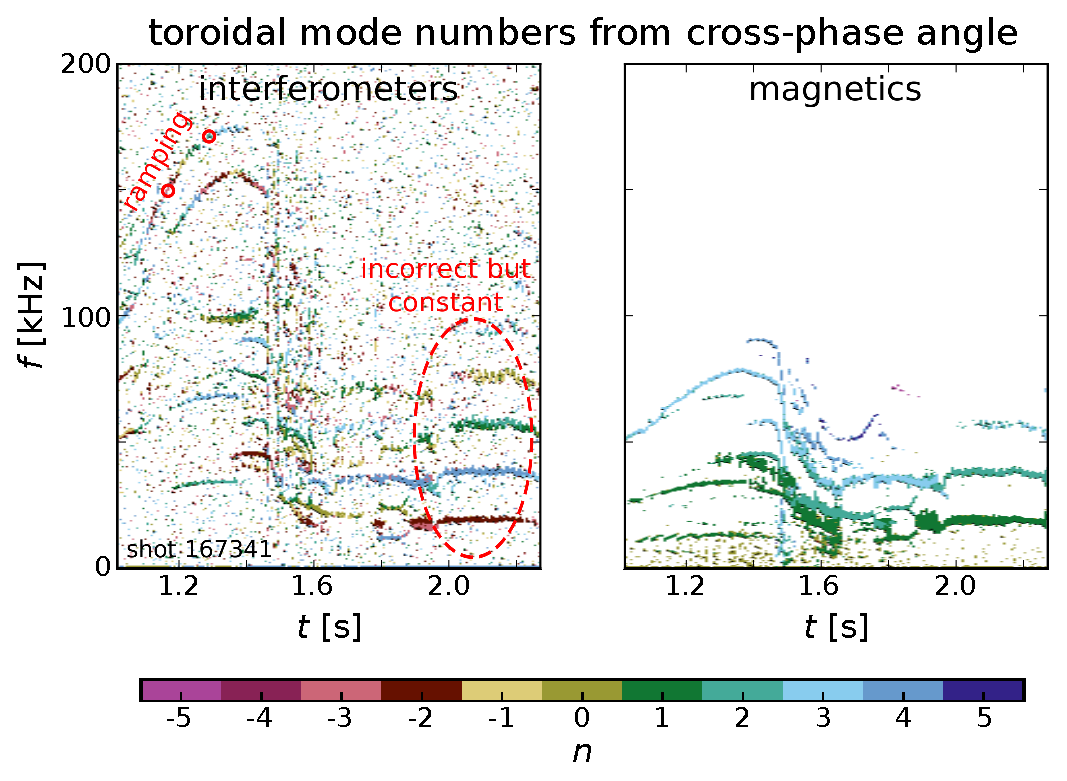
\includegraphics[width = \textwidth]{%
    Chapters/ToroidalCorrelation/figs/mode_numbers_with_uncompensated_time_delay.eps}
  \caption{Computed mode numbers from
    toroidally separated interferometers and magnetics.
    When there is an uncompensated time delay ($\delta t \neq 0$)
    between the two interferometers, as there is here,
    the interferometer-measured mode numbers
    for both constant-frequency and ramping-frequency modes
    are \emph{incorrectly} computed.}
\label{fig:ToroidalCorrelation:uncompensated_time_delay}
\end{figure}

Now, Fig.~\ref{fig:ToroidalCorrelation:uncompensated_time_delay} shows an example
of the computed toroidal mode number spectrum
when using the native time-bases of the V2 and PCI interferometers;
the corresponding magnetics spectrum is shown for comparison.
For $t \lesssim \SI{1.5}{\second}$
the mode frequencies are ramping approximately linearly in time, and
the interferometer-measured mode number is (artificially) ramping in time,
in contrast to the corresponding measurements from magnetics;
application of
(\ref{eq:ToroidalCorrelation:toroidal_mode_number_dt_ramp_rate_lab_frame})
to the \emph{highest-frequency} mode observed by the interferometers yields
$\delta t \approx \SI{-30}{\micro\second}$
($\Delta n = 5$, $\Delta f \approx \SI{20}{\kilo\hertz}$,
as indicated by the positions of the small circular annotations
to the highest frequency mode in
Fig.~\ref{fig:ToroidalCorrelation:uncompensated_time_delay}).
Further, note that the mode number evolution \emph{reverses}
after the mode reaches its peak frequency,
in agreement with the behavior expected from
(\ref{eq:ToroidalCorrelation:toroidal_mode_number_dt_ramp_rate_lab_frame}).
Finally, for $t \gtrsim \SI{2}{\second}$
the mode frequencies are constant, but
the interferometer-measured mode numbers are in disagreement with magnetics.
Naive application of
(\ref{eq:ToroidalCorrelation:toroidal_mode_number_dt_constant_omega})
to the \emph{lowest-frequency} mode at $f \approx \SI{20}{\kilo\hertz}$
yields $\delta t \approx \SI{20}{\micro\second}$
($n_{\text{meas}} = -2$, $n = 1$,
$\omega \approx 2 \pi \cdot \SI{20}{\kilo\hertz}$),
in contrast with the above time-delay estimate
from the linearly ramping mode numbers.
However, as warned above,
$n_{\text{meas}}$ will be \emph{aliased} for ``large'' time delays:
using the above parameters for the lowest-frequency mode,
we see that $|\omega \delta t / \Delta \zeta| \approx 4.8 > n_{\text{Ny}}$,
where $n_{\text{Ny}} = 4$ is the Nyquist mode number
for the $\Delta \zeta = 45^{\circ}$ toroidal separation of the interferometers,
confirming that aliasing has biased our time-delay estimate.
To account for aliasing, we can take $n_{\text{meas}} = -2 \rightarrow 6$, and
application of
(\ref{eq:ToroidalCorrelation:toroidal_mode_number_dt_constant_omega}) yields
$\delta t \approx -\SI{30}{\micro\second}$,
in agreement with the time-delay estimate
from the linearly ramping mode numbers!

The above observations are all consistent with there being an offset
between the native time-bases of the PCI and V2 interferometers, and
the two \emph{independent} measurements of this time offset are in agreement,
with each yielding an offset $\delta t \approx \SI{-30}{\micro\second}$.
Indeed, delaying the PCI signal by $-\SI{30}{\micro\second}$
relative to the V2 signal in software dramatically improves
the agreement between the interferometer and magnetics mode number spectra.
By scanning $\delta t$ about $-\SI{30}{\micro\second}$ and
noting when discrepancy with magnetics began to creep back into
the interferometer-measured mode spectrum,
the upper and lower bounds of $\delta t$ were found;
the best estimate for $\delta t$ was then taken as the midpoint
between these upper and lower bounds, which was found to be
\begin{equation}
  \delta t = -\SI{32}{\micro\second}
  \label{eq:ToroidalCorrelation:time_delay}
\end{equation}
That is, the native PCI-interferometer's time base \emph{leads}
the native V2 time base by $\SI{32}{\micro\second}$.
Delaying the PCI-interferometer by $\SI{32}{\micro\second}$ (in software)
relative to the V2 interferometer yields the mode number spectrum
shown in Fig.~\ref{fig:ToroidalCorrelation:compensated_time_delay}.
Note that both
Fig.~\ref{fig:ToroidalCorrelation:uncompensated_time_delay} and
Fig.~\ref{fig:ToroidalCorrelation:compensated_time_delay}
correspond to shot 167341, and
the only difference in the interferometer-measured mode number spectrum
between the two figures results from the compensation of the time delay
between the native time bases of the two interferometers.

\textcolor{red}{Note that additional measurements are needed
to determine which clock is correct in the \emph{absolute} sense.
For example, we can try digitizing a trigger signal and
comparing the digitized time of the trigger to the ``nominal'' trigger time
to determine the offset of our digitizer from the DIII-D clock.}

\begin{figure}
  \centering
  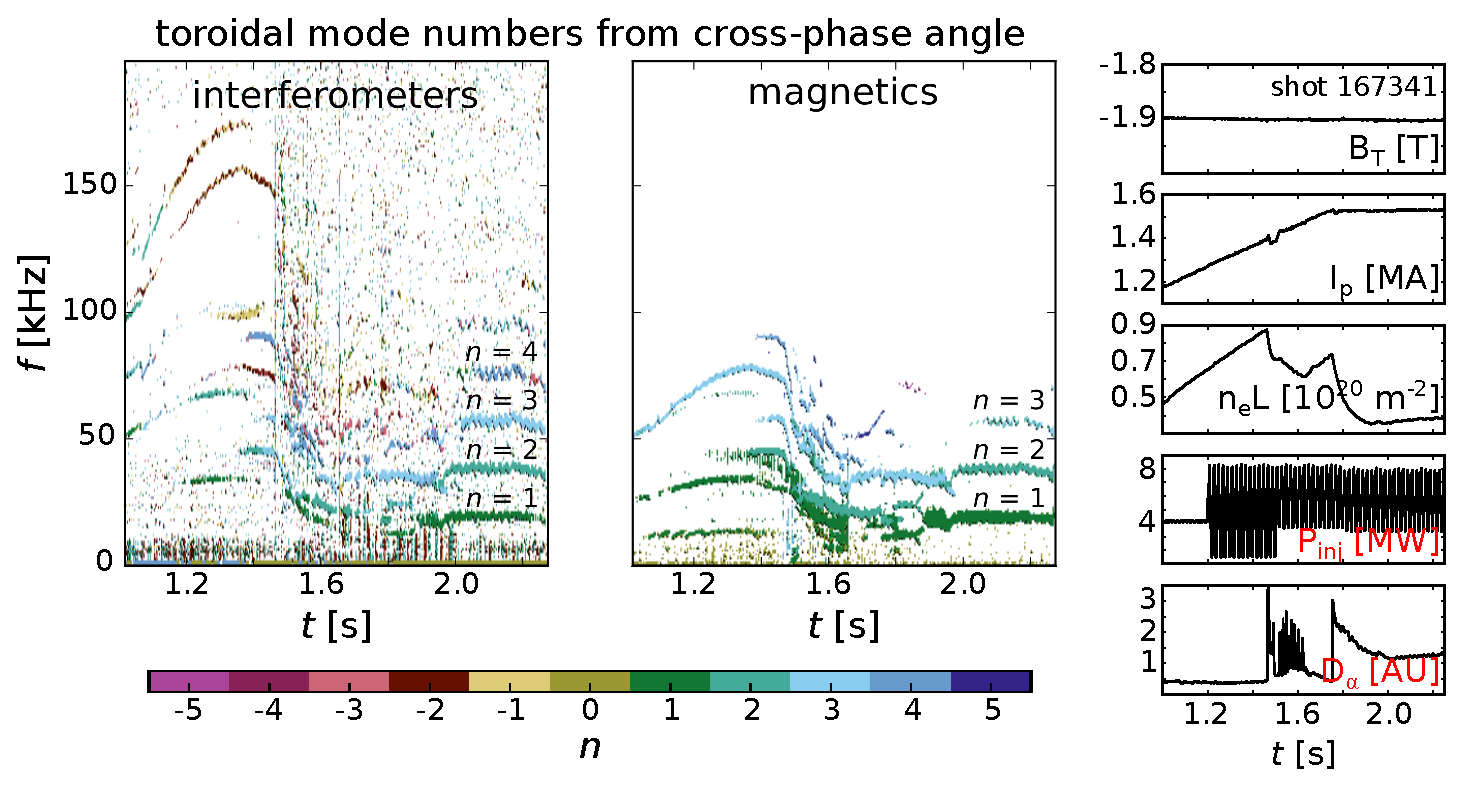
\includegraphics[width = \textwidth]{%
    Chapters/ToroidalCorrelation/figs/magnetics_and_interferometer_mode_numbers_167341.eps}
  \caption{Computed mode numbers from
    toroidally separated interferometers and magnetics.
    Here, the PCI-interferometer signal has been delayed by
    $\SI{32}{\micro\second}$ relative to the V2 signal
    to account for the time offset between each system's native time base.
    Note that the agreement with magnetics is excellent and that
    the mode numbers of the ramping-frequency modes are no longer
    artificially ramping;
    this is an enormous improvement over the corresponding
    uncompensated interferometer-measured spectrum in
    Fig.~\ref{fig:ToroidalCorrelation:uncompensated_time_delay}.}
\label{fig:ToroidalCorrelation:compensated_time_delay}
\end{figure}


\subsection{Radial offset}
The V2 and PCI interferometer beam paths have a slight radial offset
($\Delta R = \SI{4}{\centi\meter}$ with
$R_{\text{V2}} = \SI{1.94}{\meter}$ and $R_{\text{PCI}} = \SI{1.98}{\meter}$).
Thus, $\alpha_{12} = n(\zeta_2 - \zeta_1) + [\sigma(R_2) - \sigma(R_1)]$.
Recall that $\sigma_F$ is a complicated function of
the beam's major radial location,
the mode structure,
the equilibrium density profile, and
the plasma geometry.
However, the \emph{dominant} effect of such a radial offset
is attributable to the relative phase of $\vect{\xi}$
at the two radial locations:
\begin{equation}
  \sigma(R_2) - \sigma(R_1)
  \approx
  \begin{cases}
    0, & \quad \text{$\vect{\xi}(R_1)$ and $\vect{\xi}(R_2)$ in-phase} \\
    \pi, & \quad \text{$\vect{\xi}(R_1)$ and $\vect{\xi}(R_2)$ out-of-phase}
  \end{cases}
  \notag
\end{equation}
If $\vect{\xi}(R_1)$ and $\vect{\xi}(R_2)$ are in-phase,
then application of (\ref{eq:ToroidalCorrelation:toroidal_mode_number_ideal})
will yield the correct mode number.
However, if $\vect{\xi}(R_1)$ and $\vect{\xi}(R_2)$ are out-of-phase,
then application of (\ref{eq:ToroidalCorrelation:toroidal_mode_number_ideal})
will yield a measured mode number $n_{\text{meas}}$
\begin{equation}
  n_{\text{meas}}
  =
  \begin{cases}
    n + n_{\text{Ny}}, & \quad n \leq 0 \\
    n - n_{\text{Ny}}, & \quad n > 0
  \end{cases}
  \label{eq:ToroidalCorrelation:toroidal_mode_number_radially_out_of_phase}
\end{equation}
where $n_{\text{Ny}} \equiv \pi / \Delta \zeta$
is the Nyquist toroidal mode number, and
the $n > 0$ case results from \emph{aliasing}
(that is, $n + n_{\text{Ny}} \rightarrow n - n_{\text{Ny}}$
when $n > 0$ because of aliasing).
Lacking additional measurements or some type of forward modeling,
this incorrect mode-number identification may go undiagnosed.
However, if $\vect{\xi}(R)$ evolves such that
$\vect{\xi}(R_1)$ and $\vect{\xi}(R_2)$ transition
from being in-phase to being out-of-phase (or vice versa),
the measured mode number will ``flip'';
an example of this mode-number ``flipping''
is shown in Fig.~\ref{fig:ToroidalCorrelation:mode_number_flips}.
Further effects of the radial offset can be investigated
via e.g.\ forward modeling and synthetic diagnostics.

\begin{figure}
  \centering
  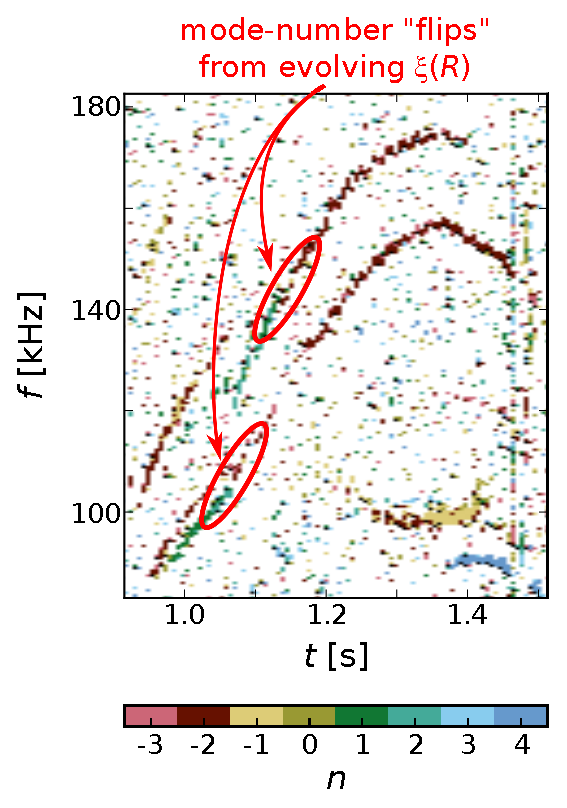
\includegraphics[width = 0.5 \textwidth]{%
    Chapters/ToroidalCorrelation/figs/phase_flips_167341.eps}
  \caption{Due to the small radial offset ($\Delta R = \SI{4}{\centi\meter}$)
    between the V2 and PCI interferometers,
    changes in the radial structure of a mode
    can result in ``flipping'' of the interferometer-measured mode number.
    Here, the mode number flips from $n = 2$ to $n = -2$,
    consistent with
    (\ref{eq:ToroidalCorrelation:toroidal_mode_number_radially_out_of_phase}).
    Lacking additional measurements or some type of forward modeling,
    it is impossible to determine if the mode is truly $n = 2$ or $n = -2$.
    Note that these modes exceed the typical bandwidth of magnetics, however,
    so even identification as $n = \pm 2$ \emph{is} an improvement!}
\label{fig:ToroidalCorrelation:mode_number_flips}
\end{figure}


\section{Example mode number spectra}

\begin{figure}[h!]
  \centering
  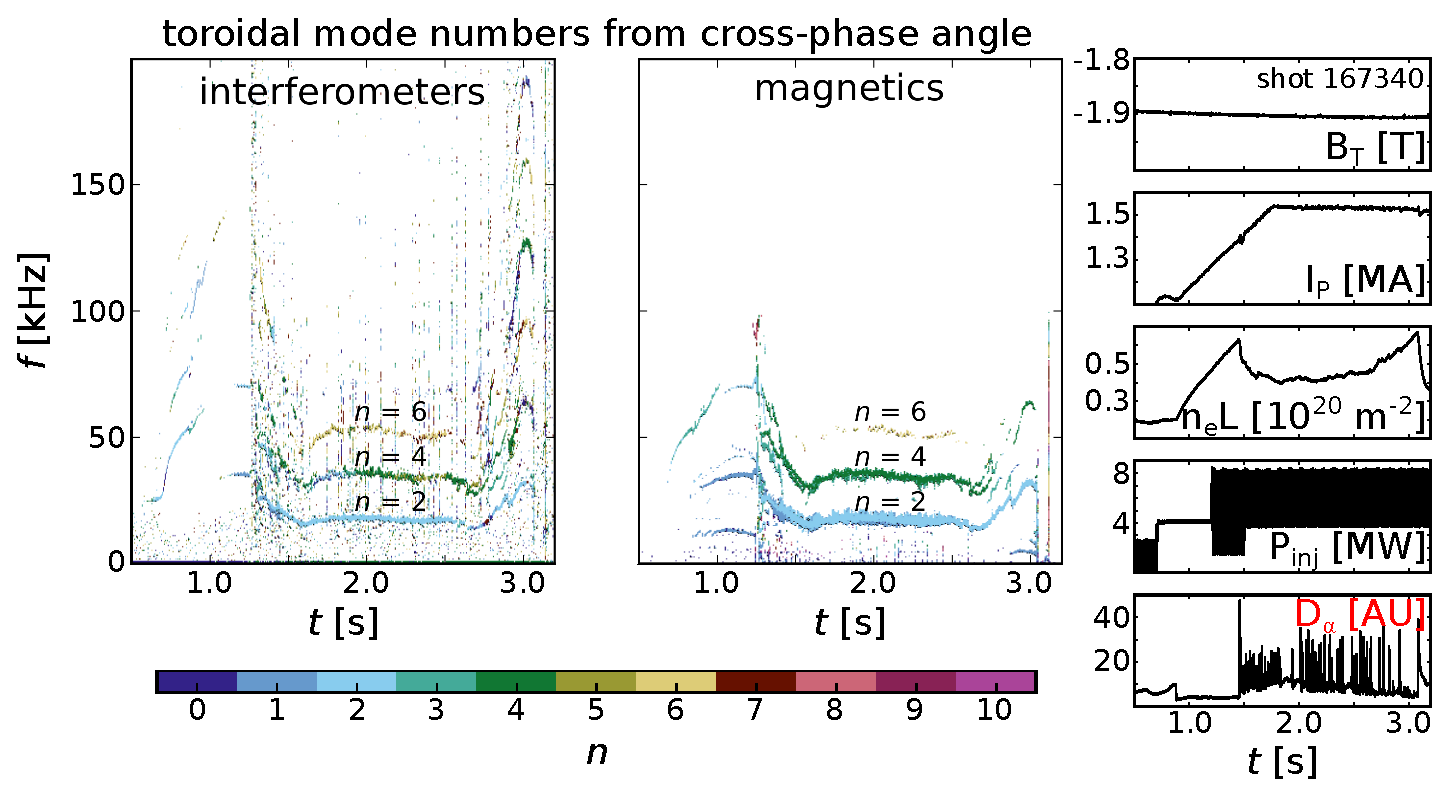
\includegraphics[width = \textwidth]{%
    Chapters/ToroidalCorrelation/figs/magnetics_and_interferometer_mode_numbers_167340.eps}
  \caption{Another example of excellent agreement between the
    interferometer and magnetics mode number spectra. Note that
    the interferometers additionally see modes \emph{invisible} to magnetics.
    Here,the modes were \emph{assumed} to be rotating
    in the ``positive'' direction
    (i.e.\ counterclockwise when viewing the torus from above,
    as this corresponds to the direction of dominant torque injection)
    such that we can discriminate $0 \leq n < 8$
    (rather than the typical $-4 < n \leq 4$).}
\label{fig:ToroidalCorrelation:magnetics_corroboration_2}
\end{figure}

\begin{figure}[h!]
  \centering
  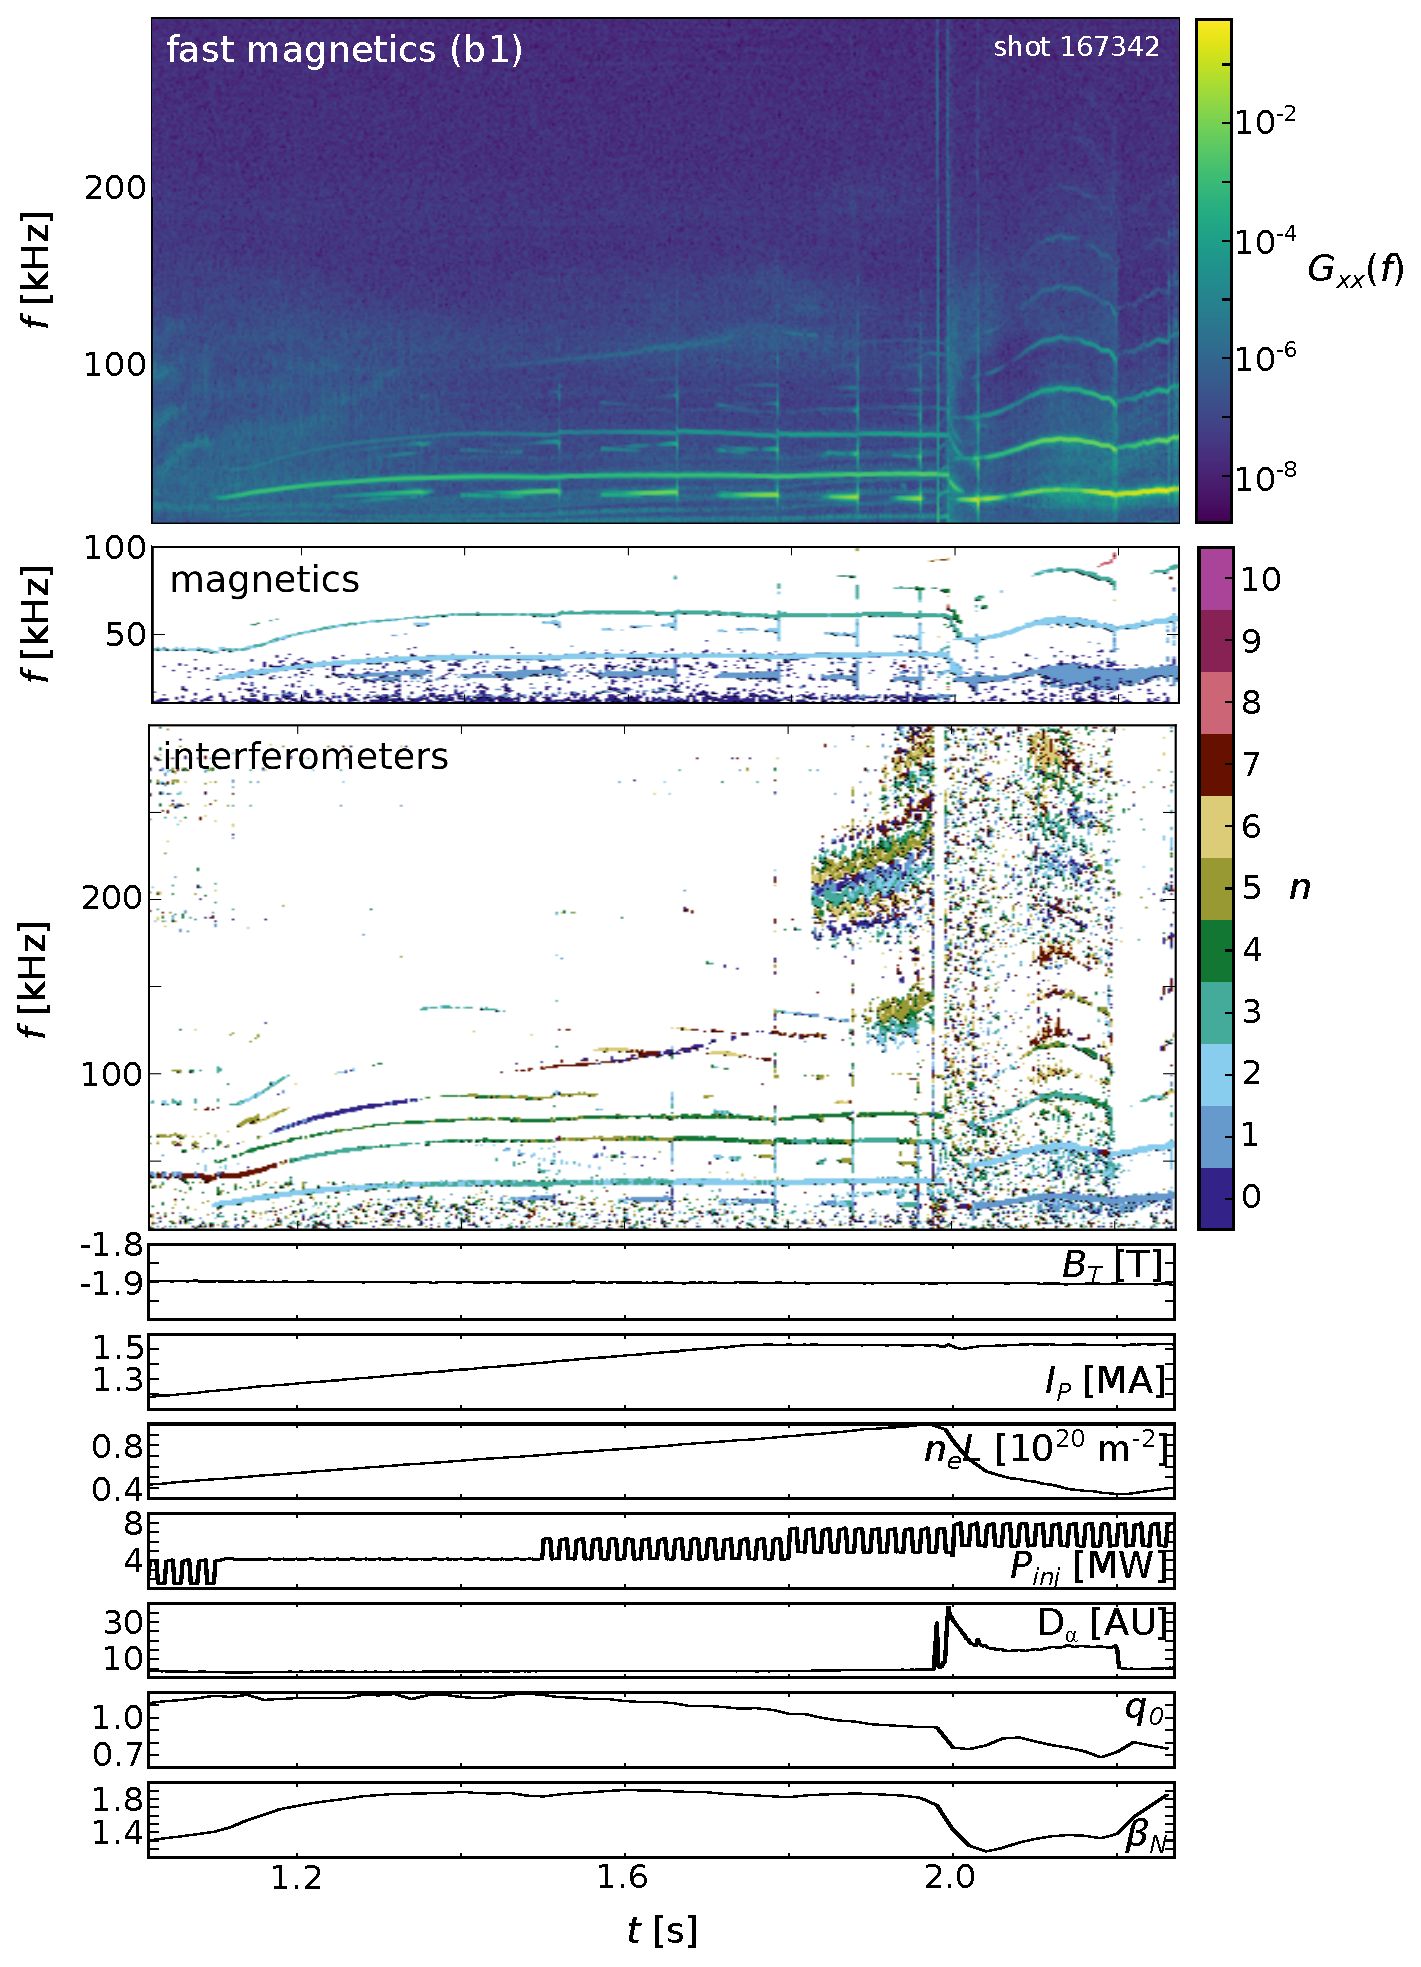
\includegraphics[width = 0.8 \textwidth]{%
    Chapters/ToroidalCorrelation/figs/core_localized_167342.eps}
  \caption{Between $1.8 \leq t \, [\text{s}] \leq 2.2$,
    the correlated interferometers measure fluctuations
    (Alfv\'{e}n eigenmodes?) that are \emph{invisible} to magnetics.
    This suggests that the modes are \emph{core-localized} and
    that the correlated interferometers are indeed capable
    of measuring core-localized MHD!
    (Note that the fast magnetic probes have a \SI{1}{\mega\hertz} bandwidth,
    but they do not have significant toroidal separation,
    preventing accurate measurement of toroidal mode numbers).}
\label{fig:ToroidalCorrelation:core_localized}
\end{figure}

\begin{figure}[h!]
  \centering
  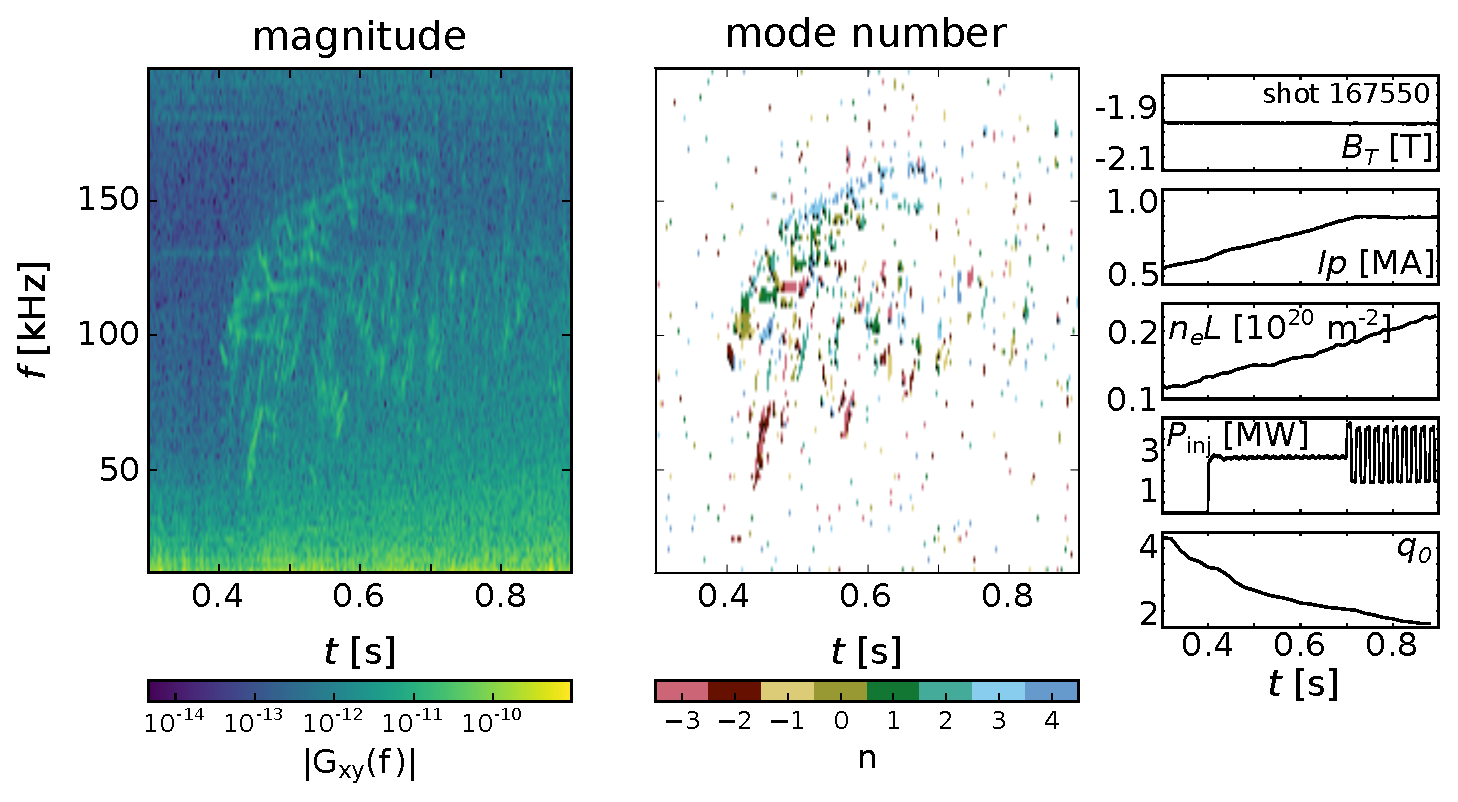
\includegraphics[width = \textwidth]{%
    Chapters/ToroidalCorrelation/figs/AEs_167550.eps}
  \caption{Alfv\'{e}n eigenmodes (?) visible
    on the correlated interferometers.
    These modes are not readily visible on magnetics.}
\label{fig:ToroidalCorrelation:AEs}
\end{figure}

\begin{figure}[h!]
  \centering
  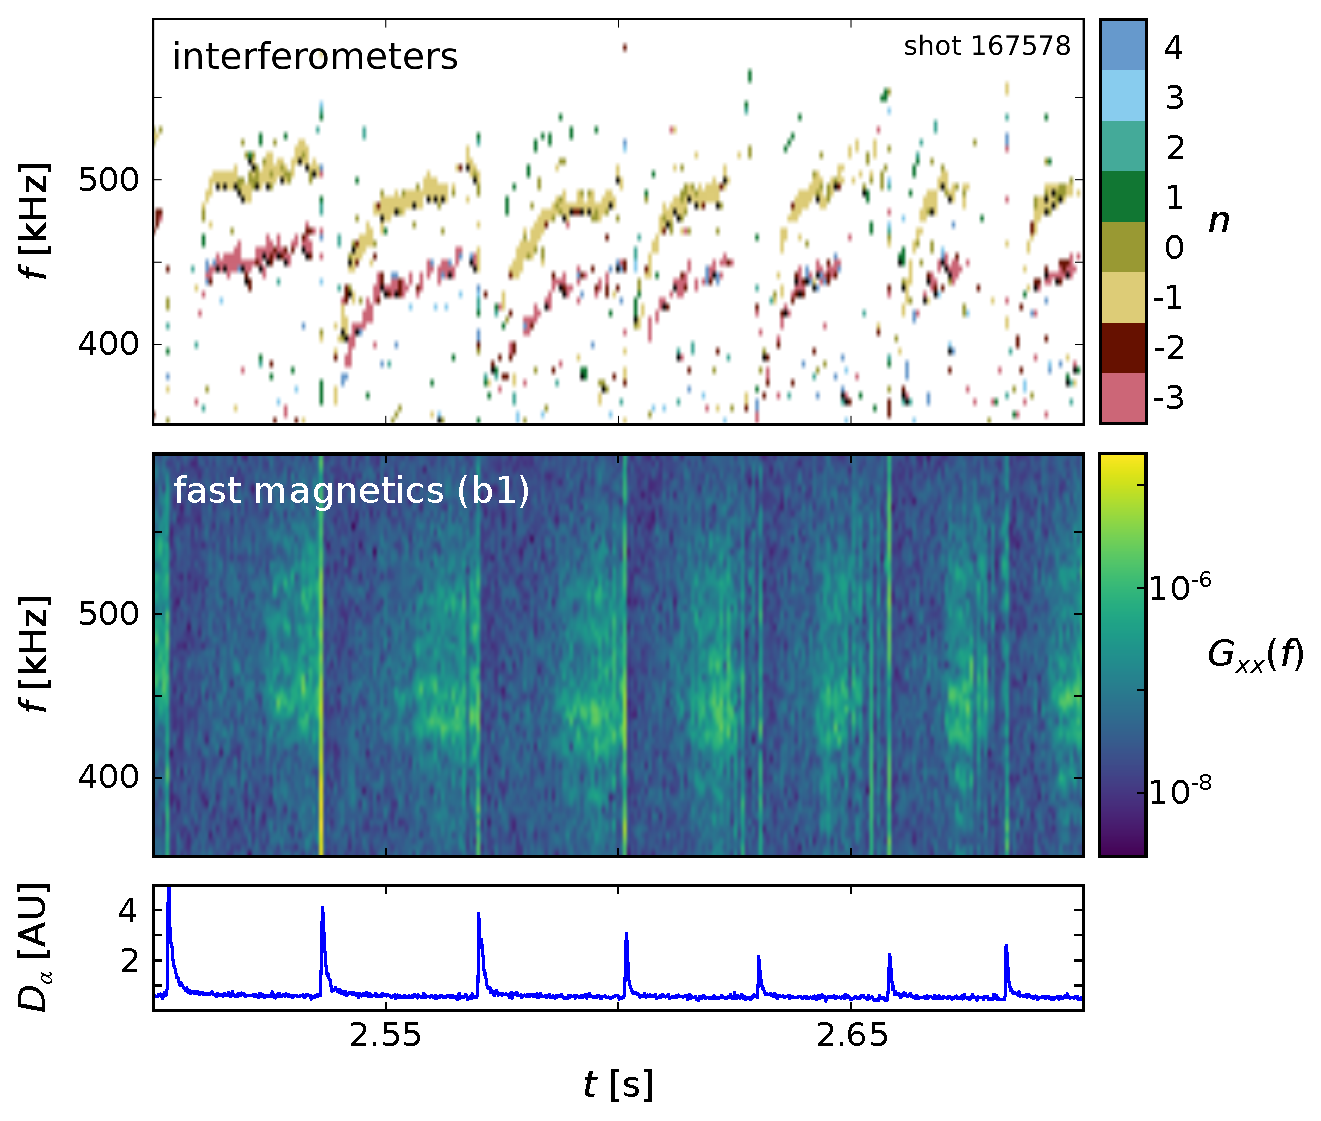
\includegraphics[width = 0.7 \textwidth]{%
    Chapters/ToroidalCorrelation/figs/interELM_fast_167578.eps}
  \caption{Inter-ELM fluctuations as measured by
    the correlated interferometers and fast magnetics.
    The mode frequency ramps early in the inter-ELM window before saturating;
    the magnetic component of the fluctuation only appears \emph{after}
    the mode frequency has saturated --- fascinating!
    (Note that the fast magnetic probes have a \SI{1}{\mega\hertz} bandwidth,
    but they do not have significant toroidal separation,
    preventing accurate measurement of toroidal mode numbers).
    The drive and significance of such fluctuations is not known, but
    they do \emph{not} occur in every ELMy discharge.}
\label{fig:ToroidalCorrelation:interELM_fast}
\end{figure}

\begin{figure}[h!]
  \centering
  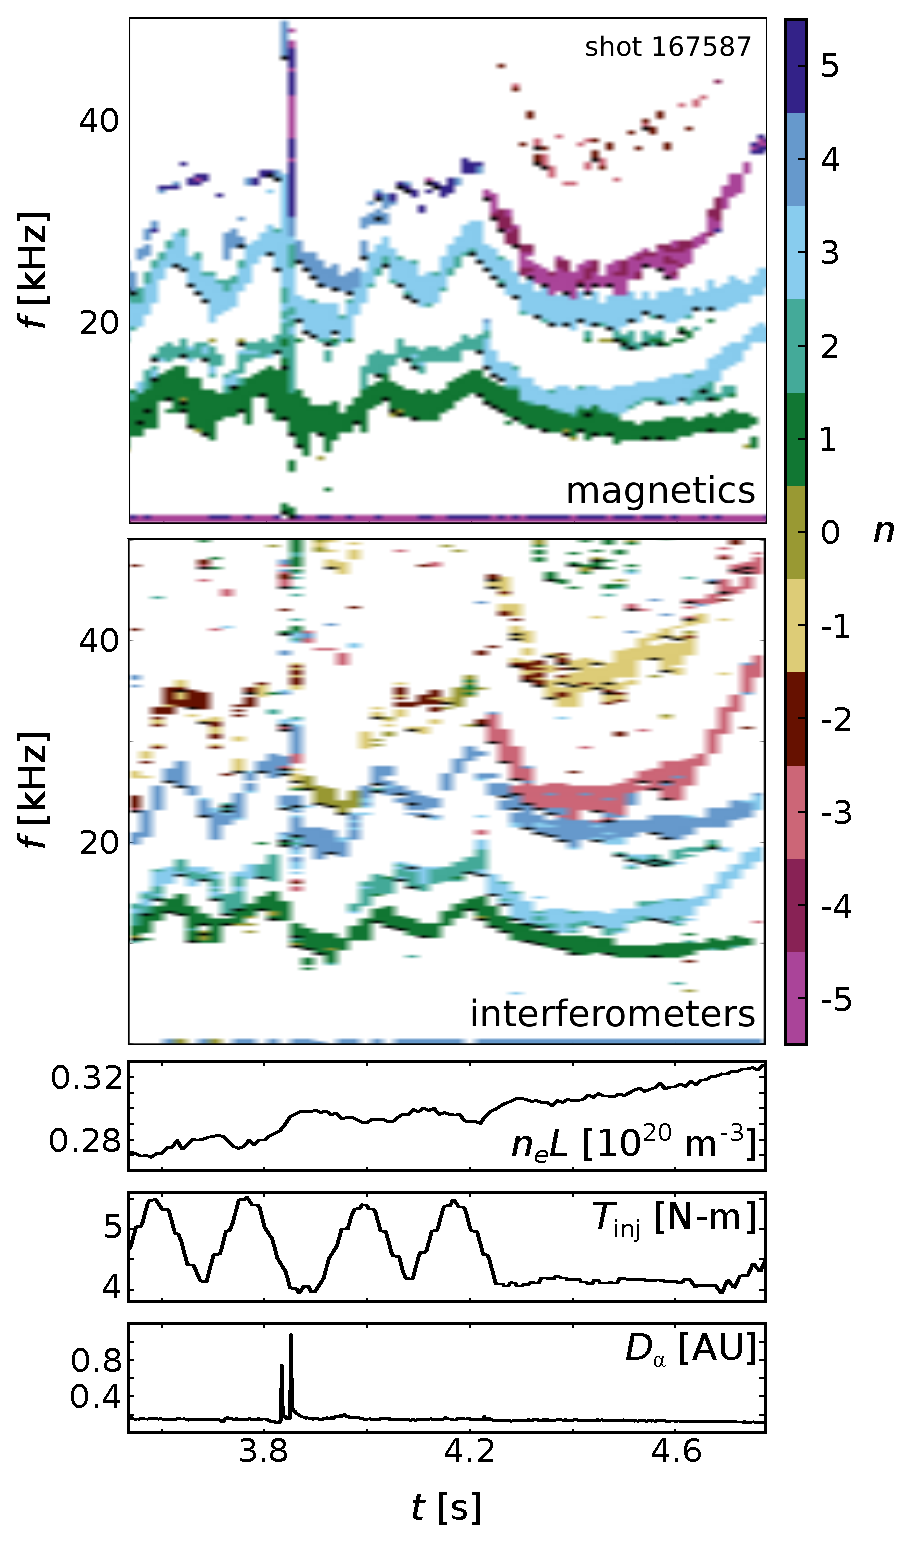
\includegraphics[width = 0.5 \textwidth]{%
    Chapters/ToroidalCorrelation/figs/EHO_167587.eps}
  \caption{The magnetics and interferometers both see the
    edge harmonic oscillation (EHO), which is responsible for
    flushing impurities from quiescent H-mode (QH-mode) plasmas.
    Below \SI{20}{\kilo\hertz}, the magnetics and interferometers
    both measure the same toroidal mode numbers; however,
    above \SI{20}{\kilo\hertz}, the measured mode numbers differ,
    likely due to a combination of aliasing and the small radial offset
    of the two interferometer beams.}
\label{fig:ToroidalCorrelation:EHO}
\end{figure}

\begin{figure}[h!]
  \centering
  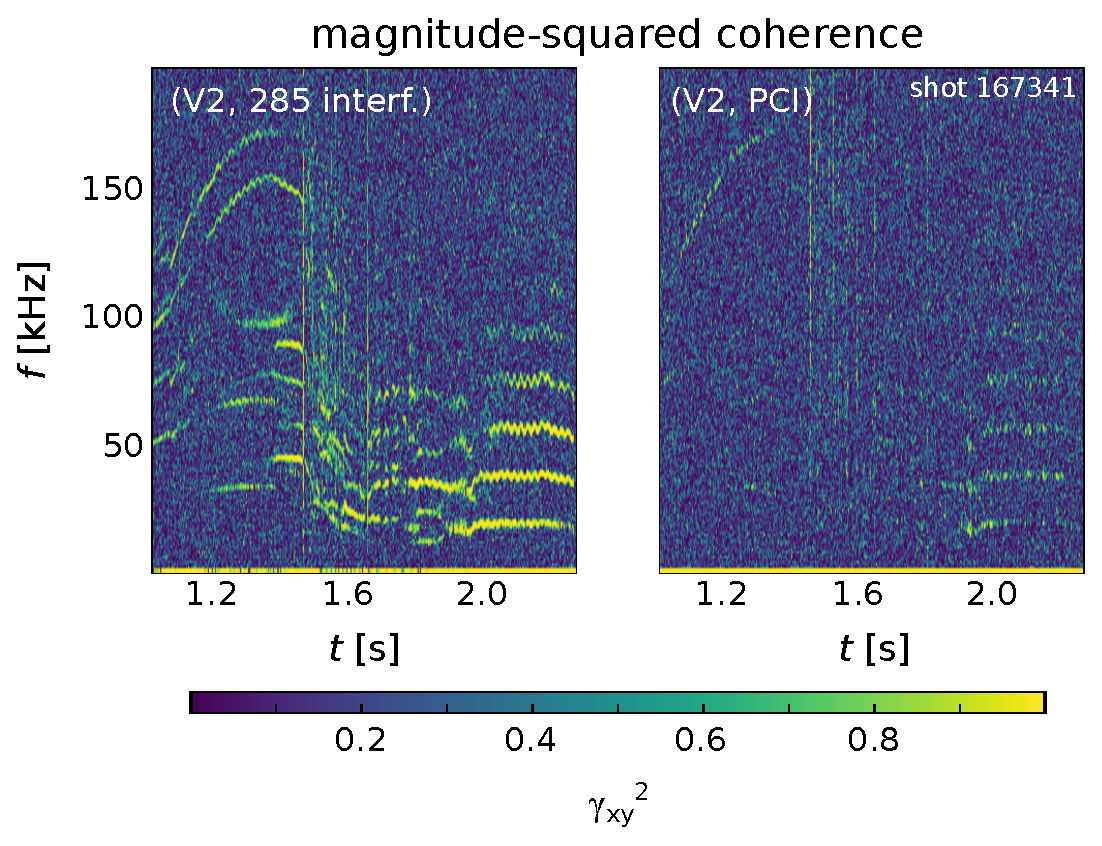
\includegraphics[width = 0.75 \textwidth]{%
    Chapters/ToroidalCorrelation/figs/interferometer_vs_PCI_coherence.eps}
  \caption[%
    Inability to correlate V2 and PCI]{%
      The magnitude-squared coherence $\gamma_{xy}^2$ between
      the V2 and 285 interferometers (left) and
      between the V2 interferometer and PCI (right).
      The high coherence between the V2 and 285 interferometers
      allows accurate measurement of toroidal mode numbers,
      as demonstrated by the corresponding mode number spectrum
      displayed in Fig.~\ref{fig:ToroidalCorrelation:compensated_time_delay},
      whereas the poor coherence between the V2 and PCI
      prevents such measurements.
      (Note that ``285 interferometer'' refers to
      the newly installed interferometer channel of the PCI).}
\label{fig:ToroidalCorrelation:PCI_coherence}
\end{figure}


\bibliographystyle{plainurl}
\bibliography{references}

\include{Chapters/FastIonTheory/FastIonTheory}
\chapter{Measurements\ldots}


See Eq.~(\ref{eq:ToroidalCorrelation:toroidal_mode_number_ideal})

\noindent See Fig.~\ref{fig:d3d_interf_layout}

\noindent See Table~\ref{table:PCI_interferometer}

\chapter{Conclusions \& future work}
\label{ch:Conclusions}


\section{Summary \& conclusions}
\label{sec:Conclusions:summary_and_conclusions}
The work described in this thesis can be summarized as follows:
\begin{itemize}
  \item Chapter~\ref{ch:InterferometricMethods} discusses
    the theory of optical interferometric methods
    in the context of measuring tokamak plasma-density fluctuations.
    The laser-plasma interaction is quantified via
    Fraunhofer scalar-diffraction theory, and
    the resulting diffracted field is imaged onto a square-law detector.
    Interfering the imaged field with a known reference field
    produces measurable intensity fluctuations;
    the specification of this reference field
    defines the interferometric method.
    Details of two particular interferometric methods ---
    external-reference-beam interferometry and
    phase contrast imaging (PCI) ---
    are discussed, with an emphasis on
    their sensitivity to fluctuations and their spatiotemporal bandwidths.
    Significantly, while PCI can measure fluctuations more sensitively
    than an external-reference-beam interferometer,
    PCI suffers from a low-$k$ cutoff;
    an external-reference-beam interferometer
    does \emph{not} suffer from such a low-$k$ cutoff.
  \item Chapter~\ref{ch:DesignConsiderations} considers the design of an
    external-reference-beam, heterodyne interferometer
    (hereafter referred to as a heterodyne interferometer).
    A criterion for satisfactory wavefront matching
    between the probe beam and the reference beam is developed, and
    finite-sampling-volume effects are shown
    to constrain the heterodyne interferometer's spatial bandwidth.
    The effects of phase noise, amplitude noise, and digitizer bit noise
    are each discussed in the context of
    the heterodyne interferometer's signal-to-noise ratio, and
    the systematic errors resulting from
    imperfect demodulation of the heterodyne interference signal
    are quantified.
  \item Chapter~\ref{ch:Implementation} details
    the addition of a heterodyne interferometer
    to the pre-existing PCI system on the \diiid\space tokamak.
    Both systems operate simultaneously,
    sharing a single $\SI{10.6}{\micro\meter}$ probe beam through the plasma.
    Optical-diagnostic access on \diiid\space and the capabilities
    of the pre-existing PCI system are briefly reviewed.
    Referencing the design considerations
    in Chapter~\ref{ch:DesignConsiderations} and
    adopting the philosophy
    that the pre-existing PCI system should be minimally perturbed,
    the optical layout for the heterodyne interferometer is developed;
    the magnification of the interferometer's imaging system
    is selected such that the spatial bandwidths
    of the PCI and interferometer have a mid-$k$ overlap.
    The design, procurement, and installation
    of the new optical and electrical components
    required to make the heterodyne interferometric measurement
    are summarized.
    Of note is the interferometer's radio-frequency local oscillator:
    the phase noise of a crystal oscillator (XO)
    was empirically found to be \emph{too large}
    to make meaningful fluctuation measurements in most tokamak plasmas, but
    the substantially lower phase noise of an
    oven-controlled crystal oscillator (OCXO)
    allows measurements of a whole zoo
    of coherent and broadband plasma fluctuations.
    The interferometer response and
    the multiscale capabilities of the combined PCI-interferometer
    are empirically verified via sound-wave calibrations.
    Specifically, the PCI is shown to measure high-$k$
    ($\SI{1.5}{\per\centi\meter} < |k_R| \leq \SI{25}{\per\centi\meter}$)
    fluctuations with
    sensitivity $3 \times 10^{13} \; \text{m}^{-2} / \sqrt{\text{kHz}}$,
    while the interferometer simultaneously measures low-$k$
    ($|k_R| < \SI{5}{\per\centi\meter}$) fluctuations with
    sensitivity $3 \times 10^{14} \; \text{m}^{-2} / \sqrt{\text{kHz}}$.
    Both systems have temporal bandwidths in excess of $\SI{1}{\mega\hertz}$.
  \item Chapter~\ref{ch:TurbulenceMeasurements} demonstrates
    the multiscale capabilities of the combined PCI-interferometer.
    During a recent \diiid\space experiment,
    the location of electron cyclotron resonance heating (ECH)
    was moved from $\rhoech = 0.5$ to $\rho_{ECH} = 0.8$,
    altering the local $a / L_{T_e}$ and $a / L_{T_i}$
    in an attempt to change the coupling between
    the electron-scale and ion-scale turbulence.
    As such, this experiment presents an ideal opportunity
    for multiscale turbulence investigations
    with the combined PCI-interferometer.
    Numerous turbulent branches are observed.
    In particular, the interferometer measures
    a low-$k$ electromagnetic mode driven unstable by collisionality,
    properties consistent with the micro-tearing mode (MTM), and
    the PCI measures a wavenumber spectrum
    that exhibits distinct flattening
    when $a / L_{T_e}$ is increased relative to $a / L_{T_i}$,
    reminiscent of results
    from realistic multiscale gyrokinetic simulations~\cite{howard_pp16}.
    To aid the interpretation of these measurements,
    linear-stability analysis and quasilinear-transport modeling
    are performed with the gyro-Landau fluid code TGLF, and
    qualitative agreement with the PCI-measured wavenumber spectrum
    is obtained.
  \item Chapter~\ref{ch:ToroidalCorrelation} discusses the correlation
    of the newly installed interferometer with
    \diiid's toroidally separated, pre-existing $V2$ interferometer.
    Capable of probing the core plasma,
    the interferometers are shown to be sensitive
    to core-localized fluctuations
    that are \emph{invisible} to external magnetic probes.
    The chapter begins with a brief review
    of the two-point correlation technique and
    shows how toroidal mode numbers can be extracted
    from a pair of toroidally separated measurements.
    Meaningful correlation requires that
    the two measurements share the same timebase.
    The digitizers of both interferometers were modified
    to phase lock their clocks, and
    a residual ``trigger offset'' was measured
    and is compensated in software.
    Where comparisons can be made with magnetic probes,
    the interferometer-measured toroidal mode numbers
    are in good agreement.
    Currently, there is not a tested, robust method
    for correcting the bias introduced by
    the $\SI{4}{\centi\meter}$ major-radial offset
    between the interferometer beam centers,
    which unfortunately limits the
    deployment of this system for physics studies
    of core-localized MHD.
\end{itemize}


\section{Future work}
\label{sec:Conclusions:future_work}
The combined PCI-interferometer developed in this work
has a clear application in the burgeoning study
of multiscale turbulence and cross-scale coupling, which
may be significant in the reactor relevant $T_e \approx T_i$ regime.
In roughly the next six months,
Howard \emph{et al.} expects to complete
realistic multiscale gyrokinetic simulations
for the experiment described in
Chapter~\ref{ch:TurbulenceMeasurements}.
It will be very interesting
to see if the predicted wavenumber spectrum
matches the PCI-measured wavenumber spectrum.
It should be noted that a synthetic PCI diagnostic
already exists for the interpretation
of such gyrokinetic simulations~\cite{rost_pp10}.
Small modifications to the synthetic PCI
should also allow a synthetic interferometer diagnostic.
Previous multiscale simulations predict
significant local and non-local energy cascades
between the ion and electron scales~\cite{howard_pp16}, so
it is desirable to investigate such coupling empirically.
With its large spatiotemporal bandwidth,
the combined PCI-interferometer may be ideally suited
for measurement of such coupling, which
may be suitably quantified by
the bicoherence~\cite{young_and_powers_ieee79}
between various channels of the system or
some other suitable measure of nonlinear processes.
(Note that the author has performed preliminary bispectral analysis
of the measurements discussed in
Chapter~\ref{ch:TurbulenceMeasurements};
interestingly, the $|k_R| \sim \SI{5}{\per\centi\meter}$ and
$f \sim \SI{1}{\mega\hertz}$ mode observed in
Figure~\ref{fig:TurbulenceMeasurements:Skf_pci}(b)
has an exceptionally large autobicoherence).

The interferometer-measured, low-$k$, electromagnetic modes
that are destabilized by collisionality
are also deserving of further study.
The properties of this mode are consistent
with the micro-tearing mode, which
was predicted to be marginally unstable
in the multiscale experiment's reference discharge~\cite{holland_nf17}.
Unfortunately, TGLF's default eigenfunction basis
of four Hermite polynomials is typically insufficient
to resolve micro-tearing modes (MTMs)~\cite{staebler_MTM_question}, so
there are no attempts to simulate the MTM in this work.
However, it may be conceivable that
increasing the number of Hermite polynomials
will allow identification of the MTM in TGLF.
Alternatively, linear simulations with
the gyrokinetic code GYRO~\cite{candy_jcp03}
could be pursued.
(Note that the reference-discharge simulations
indicating marginal MTM instability were performed with GYRO).
Experimentally, it is desirable to map out the parametric dependencies
of this mode, particularly its response
to the plasma $\beta$ and collisionality.
If dedicated experiments cannot be performed,
it should be noted that the relevant experimental conditions
(i.e.\ ITER-baseline scenario) are fairly typical at \diiid, and
a fair amount may still be learned
by ``piggybacking'' on other experiments.

With regards to the combined PCI-interferometer,
the most substantial improvement to the system
would be upgrading the heterodyne-interferometer detector
from a single element to a multi-element array.
This would allow reconstruction of $k_R$
from the interferometer measurements,
enabling estimates of
frequency-wavenumber spectra $S_{\phi,\phi}(k,f)$ and
wavenumber spectra $S_{\phi,\phi}(k)$
much like with the PCI.
This capability is desirable for several reasons.
First and foremost,
interferometric measurements across a multi-element array
would allow accurate estimates of $S_{\phi,\phi}(k)$
below the PCI low-$k$ cutoff
(\ref{eq:Implementation:kg_realized}), which
may have important implications for
validation of spectral-flattening predictions
from multiscale gyrokinetic predictions.
Further, as discussed in
Section~\ref{sec:Implementation:Calibration:pci},
interferometric measurements across a multi-element array
would allow robust and accurate
cross-calibration of the PCI
on a shot-to-shot and an intra-shot basis.
Note that each additional detector element
would require its own set of electronics
(e.g.\ signal conditioning RF amplifiers,
demodulation electronics, and
audio amplifiers) and
two additional digitizer channels
(to digitize both the in-phase $I$ and quadrature $Q$ signals).
While the ``deadbug'' circuit construction utilized in this work
is ideal for prototyping,
any future increase to the number of interferometer channels
would call for a printed-circuit-board (PCB) construction
of the electronics.
Thus, increasing the number of interferometer channels
is not a small undertaking.

A simpler, cheaper, and faster performance improvement
would be the procurement of anti-aliasing filters
with a higher cutoff frequency.
The current anti-aliasing filters
limit the bandwidth of the interferometer to
approximately $\SI{1}{\mega\hertz}$, but
the upstream components have bandwidths
in excess of $\SI{2}{\mega\hertz}$.
Thus, new anti-aliasing filters could,
quite literally overnight,
nearly double the temporal bandwidth of the interferometer.

Finally, there is not currently a tested, robust method
for correcting the bias introduced by
the major-radial offset of the toroidally correlated interferometers
(other than reducing the offset, i.e.\ $\Delta R \rightarrow 0$,
which is not possible with current port allocations).
It may be possible to account for the radial and poloidal mode structure
via e.g.\ measurements from
microwave imaging reflectometry (MIR)~\cite{muscatello_rsi14} or
electron cyclotron emission imaging (ECEI)~\cite{tobias_rsi10}.

Looking towards ITER and other next-step devices,
the combined PCI-interferometer may allow
sensitive, high spatiotemporal bandwidth measurements
of multiscale turbulence.
The diagnostic development pursued in this thesis
proves that heterodyne-interferometric detection and PCI detection
can be simultaneously implemented
using a shared probe beam and
a shared set of ports.
The addition of PCI detection to
e.g.\ the ITER interferometer~\cite{vanzeeland_TIP_rsi13}, however,
is not without its challenges.
For example, the ITER interferometer
employs a Michelson configuration,
with the beam making a second pass through the plasma
after bouncing off of a retroreflector inside the vacuum vessel.
In contrast,
at least to the author's knowledge,
all previous PCI implementations
have employed a Mach-Zehnder configuration,
with the probe beam making a single pass through the plasma.
In principle, PCI can use a Michelson configuration, but
the double pass and retroreflector
may complicate interpretation of the measurements,
particularly if attempting to localize the measurements
with a spatially filtering mask~\cite{dorris_rsi09, dorris_phd, lin_rsi06} or
with $2$-dimensional detector arrays~\cite{sanin_rsi04, tanaka_rsi16}.

Regardless, the spatial bandwidth of a PCI system
that shares its probe beam
with the ITER interferometer can be considered.
The 1/e $E$ waist of the ITER interferometer's
$\SI{10.6}{\micro\meter}$ probe beam is
$w_0 \approx \SI{8}{\milli\meter}$~\cite{vanzeeland_TIP_rsi13}
such that a PCI system using this probe beam
would have a diffraction-limited low-$k$ cutoff
(\ref{eq:InterferometricMethods:pci_kmin_physics})
of $\SI{2.5}{\per\centi\meter}$.
(However, recall that the \diiid\space PCI
is operated two to three times above the diffraction limit
to give some leeway to the PCI feedback system).
Of course, as demonstrated in this thesis,
simultaneous heterodyne-interferometric and PCI detection
can obviate the PCI's low-$k$ cutoff.
A somewhat larger problem, however, may be the limited collection volumes
and long path lengths
between the vacuum vessel and the detector, which
may impose severe constraints
on the high-$k$ cutoff of a $\SI{10.6}{\micro\meter}$ PCI or interferometer.
One potential solution is to use a smaller probe wavelength
(i.e.\ larger $k_0$) to decrease the scattering angle $\theta_m$ from
(\ref{eq:GaussianBeamDiffraction:scattering_angles}).
As the burning plasma regime will be predominantly electron heated
(i.e.\ via fusion alpha particles slowing down on electrons),
it is extremely important that
both high-$k$ electron turbulence and
any cross-scale coupling with low-$k$ ion turbulence
is accurately diagnosed and understood.


\bibliographystyle{plainurl}
\bibliography{references}



% **********
% Backmatter
% **********
\appendix
\cleardoublepage
\chapter{Some identities for the PCI wavenumber response}
\label{app:PCIResponseIdentities}


\section{Phase factor in the beam's near field}
The effect of wavenumber-dependent manipulation $T(k_x)$
on the $m$\ts{th} scattered beam is given by
the phase factor $\mathcal{P}(m, k, x)$ as defined in
(\ref{eq:InterferometricMethods:mth_diffracted_beam_kx_filtered_phase_factor}),
which is repeated here for completeness
\begin{equation}
  \begin{aligned}
    \mathcal{P}(m, k, x)
    &=
    \frac{1}{2 \pi}
    \int dx' \,
    \exp\left[ \frac{-x'^2}{w(z)^2} \right]
    \exp\left\{%
      i \left[%
        m k x'
        +
        \frac{k_0 x'^2}{2 R(z)}
      \right]
    \right\}
    \\
    &\qquad \times
    \int dk_x' \,
    T(k_x')
    e^{i k_x' (x_m - x')}
  \end{aligned}
  \label{eq:PCIResponseIdentities:mth_diffracted_beam_kx_filtered_phase_factor_full}
\end{equation}
The integrals are over the full domain of $x'$ and $k_x'$, but
note that contributions to the integral
from regions outside of $|x'| \lesssim w(z)$
are suppressed by the Gaussian envelope such that
the maximum value of the curvature-induced phase factor obeys
\begin{equation}
  \left[ \frac{k_0 x'^2}{2 R(z)} \right]_{\text{max}}
  \sim
  \frac{k_0 [w(z)]^2}{2 R(z)}
  \label{eq:PCIResponseIdentities:curvature_phase_factor_constraint_general}
\end{equation}
Now, in the beam's near field
($z \ll z_R$, which is often experimentally relevant),
the beam's waist and radius of curvature are
\begin{align}
  w(z) &\approx w_0
  \\
  R(z) &\approx \frac{z_R^2}{z}
\end{align}
as can be easily verified by examining the definitions in
(\ref{eq:InterferometricMethods:Gaussian_beam_width}) and
(\ref{eq:InterferometricMethods:Gaussian_beam_radius_of_curvature}),
respectively.
Thus,
(\ref{eq:PCIResponseIdentities:curvature_phase_factor_constraint_general})
becomes
\begin{align}
  \left[ \frac{k_0 x'^2}{2 R(z)} \right]_{\text{max}}
  &\sim
  \frac{k_0 [w(z)]^2}{2 R(z)}
  \notag \\
  &\approx
  \frac{k_0 w_0^2}{2 (z / z_R)}
  \notag \\
  &= \frac{z}{z_R}
  \notag \\
  &\ll 1
  \label{eq:PCIResponseIdentities:curvature_phase_factor_constraint_near_field}
\end{align}
where $z / z_R \ll 1$ follows from the near-field assumption.
Thus, in the beam's near field,
the curvature-induced phase factor is negligible, and
$\mathcal{P}(m, k, x)$ reduces to
\begin{equation}
  \begin{aligned}
    \mathcal{P}(m, k, x)
    &=
    \frac{1}{2 \pi}
    \int dx' \,
    e^{-\left[ x' / w(z) \right]^2}
    e^{i m k x'}
    \\
    &\qquad \times
    \int dk_x' \,
    T(k_x')
    e^{i k_x' (x_m - x')}
  \end{aligned}
  \label{eq:PCIResponseIdentities:mth_diffracted_beam_kx_filtered_phase_factor_near_field}
\end{equation}
This near-field assumption will be implicit
in the remainder of the discussion about PCI.


\section{The PCI phase factor}
The transfer function of the PCI phase plate can be described as
\begin{equation}
  \begin{aligned}
    T(k_x)
    &=
    i \sqrt{\eta} \, H(k_g - |k_x|)
    \\
    &\quad +
    H(|k_x| - k_g)
    H(k_D - |k_x|)
  \end{aligned}
  \label{eq:PCIResponseIdentities:phase_plate_transfer_function}
\end{equation}
where $H(x)$ is the Heaviside step function defined as
\begin{equation}
  H(x)
  =
  \begin{cases}
    0, \quad &x < 0 \\
    1, \quad &x \geq 0
  \end{cases}
  \label{eq:PCIResponseIdentities:Heaviside_step_function}
\end{equation}
$\eta$ is the reflectivity of the phase-plate groove, and
$k_g$ and $k_D$ are the low-$k$ and high-$k$ cutoffs of the phase plate
as defined in
(\ref{eq:InterferometricMethods:pci_kmin_engineering}) and
(\ref{eq:InterferometricMethods:pci_kmax_engineering}), respectively.
Note that the first term on the right-hand side of
(\ref{eq:PCIResponseIdentities:phase_plate_transfer_function})
corresponds to reflection from the phase-plate groove, while
the second term corresponds to reflection
from the non-grooved portion of the phase plate (i.e.\ the ``face'').
Thus, the PCI phase factor $\mathcal{P}(m, k, x)$ is
\begin{equation}
  \begin{aligned}
    \mathcal{P}(m, k, x)
    &=
    \frac{1}{2 \pi}
    \int dx' \,
    e^{-\left[ x' / w(z) \right]^2}
    e^{i m k x'}
    \\
    &\begin{aligned}
      \quad
      \times
      \Biggl\{%
        &\int_{-k_D}^{-k_g} dk_x' \,
        e^{i k_x' (x_m - x')}
        \\
        &+
        i \sqrt{\eta}
        \int_{-k_g}^{k_g} dk_x' \,
        e^{i k_x' (x_m - x')}
        \\
        &+
        \int_{k_g}^{k_D} dk_x' \,
        e^{i k_x' (x_m - x')}
      \Biggr\}
    \end{aligned}
  \end{aligned}
  \label{eq:PCIResponseIdentities:mth_diffracted_beam_kx_filtered_phase_factor_near_field_integrals}
\end{equation}


\section{Some useful integrals for evaluation of $\mathcal{P}(m, k, x)$}


\subsection{Finite-domain inverse Fourier transforms of unity}
Note that
\begin{equation}
  \int_{k_1}^{k_2} dk_x
  e^{i k_x x}
  =
  \frac{e^{i k_2 x} - e^{i k_1 x}}{ix}
\end{equation}
Now, if $k_1 = -k_2$, this simplifies to
\begin{equation}
  \int_{-k_2}^{k_2} dk_x
  e^{i k_x x}
  =
  2 k_2 \sinc \left( \frac{k_2 x}{\pi} \right)
  \label{eq:PCIResponseIdentities:finite_domain_inverse_FT_groove}
\end{equation}
where
\begin{equation}
  \sinc(x) = \frac{\sin(\pi x)}{\pi x}
  \label{eq:PCIResponseIdentities:normalized_sinc}
\end{equation}
is the normalized sinc function;
note that sinc is an \emph{even} function.
Finally, note that
\begin{align}
  \int_{-k_2}^{-k_1}
  &dk_x
  e^{i k_x x}
  +
  \int_{k_1}^{k_2} dk_x
  e^{i k_x x}
  \notag \\
  &=
  \int_{-k_2}^{k_2} dk_x
  e^{i k_x x}
  -
  \int_{-k_1}^{k_1} dk_x
  e^{i k_x x}
  \notag \\
  &=
  2 k_2 \sinc \left( \frac{k_2 x}{\pi} \right)
  -
  2 k_1 \sinc \left( \frac{k_1 x}{\pi} \right)
  \label{eq:PCIResponseIdentities:finite_domain_inverse_FT_face}
\end{align}
Using (\ref{eq:PCIResponseIdentities:finite_domain_inverse_FT_groove}) and
(\ref{eq:PCIResponseIdentities:finite_domain_inverse_FT_face}),
it is easy to see that
(\ref{eq:PCIResponseIdentities:mth_diffracted_beam_kx_filtered_phase_factor_near_field_integrals})
becomes
\begin{equation}
  \begin{aligned}
    \mathcal{P}(m, k, x)
    &=
    \frac{1}{\pi}
    \int dx' \,
    e^{-\left[ x' / w(z) \right]^2}
    e^{i m k x'}
    \\
    &\begin{aligned}
      \quad
      \times
      \Biggl\{%
        &k_D \sinc\left[ \frac{k_D}{\pi} (x' - x_m) \right]
        \\
        &-
        k_g \sinc\left[ \frac{k_g}{\pi} (x' - x_m) \right]
        \\
        &+
        i \sqrt{\eta}
        k_g \sinc\left[ \frac{k_g}{\pi} (x' - x_m) \right]
      \Biggr\}
    \end{aligned}
  \end{aligned}
  \label{eq:PCIResponseIdentities:mth_diffracted_beam_kx_filtered_phase_factor_near_field_sincs}
\end{equation}


\subsection{Integral of offset sinc with complex-Gaussian weighting}
Note that
(\ref{eq:PCIResponseIdentities:mth_diffracted_beam_kx_filtered_phase_factor_near_field_sincs})
consists of several integrals of the form
\begin{equation}
  I
  \equiv
  \frac{b}{\pi}
  \int dx \,
  e^{-a x^2}
  e^{i c x}
  \sinc\left[ \frac{b}{\pi} (x - x_0) \right]
  \label{eq:PCIResponseIdentities:I_x0_abc_definition}
\end{equation}
where $a > 0$ and $x_0$, $b$, and $c$ are real.
While daunting, the integral can be evaluated ``analytically''
in terms of complex error functions as follows
\begin{align}
  I
  &=
  \frac{b}{\pi}
  \int dx \,
  e^{-a x^2}
  e^{i c x}
  \sinc\left[ \frac{b}{\pi} (x - x_0) \right]
  \notag \\
  &=
  \frac{1}{\pi}
  \int dx \,
  e^{-a x^2}
  e^{i c x}
  \cdot
  \frac{\sin[b (x - x_0)]}{x - x_0}
  \notag \\
  &=
  \frac{1}{\pi}
  \int_{0}^{b} d\beta
  \int dx \,
  e^{-a x^2}
  e^{i c x}
  \cos[\beta (x - x_0)]
  \notag \\
  &=
  \frac{1}{2 \pi}
  \int_{0}^{b} d\beta
  \int dx \,
  e^{-a x^2}
  e^{i c x}
  \left[%
    e^{i \beta (x - x_0)}
    +
    e^{-i \beta (x - x_0)}
  \right]
  \notag \\
  &\begin{aligned}
    &=
    \frac{1}{2 \pi}
    \int_{0}^{b} d\beta
    \int dx \,
    e^{-a x^2}
    e^{i [(\beta + c) x - \beta x_0]}
    \\
    &\quad+
    \frac{1}{2 \pi}
    \int_{0}^{b} d\beta
    \int dx \,
    e^{-a x^2}
    e^{i [-(\beta - c) x + \beta x_0]}
  \end{aligned}
  \notag \\
  &\begin{aligned}
    &=
    \frac{1}{2 \pi}
    \int_{0}^{b} d\beta
    \int dx \,
    e^{-a x^2}
    e^{i [(\beta + c) x - \beta x_0]}
    \\
    &\quad-
    \frac{1}{2 \pi}
    \int_{0}^{-b} d\beta'
    \int dx \,
    e^{-a x^2}
    e^{i [(\beta' + c) x - \beta' x_0]}
  \end{aligned}
  \notag \\
  &=
  \frac{1}{2 \pi}
  \int_{-b}^{b} d\beta
  \int dx \,
  e^{-a x^2}
  e^{i [(\beta + c) x - \beta x_0]}
  \notag \\
  &=
  \frac{1}{2 \pi}
  \int_{-b}^{b} d\beta \,
  e^{-(\beta + c)^2 / 4 a}
  e^{-i \beta x_0}
  \int dx \,
  e^{-a [x - i (\beta + c) / 2a]^2}
  \notag \\
  &=
  \frac{1}{2 \sqrt{\pi a}}
  \int_{-b}^{b} d\beta \,
  e^{-(\beta + c)^2 / 4 a}
  e^{-i \beta x_0}
  \notag \\
  &=
  \frac{1}{2 \sqrt{\pi a}}
  e^{i c x_0}
  \int_{c - b}^{c + b} d\beta' \,
  e^{-\beta'^2 / 4 a}
  e^{-i \beta' x_0}
  \notag \\
  &=
  \frac{1}{2 \sqrt{\pi a}}
  e^{-a x_0^2}
  e^{i c x_0}
  \int_{c - b}^{c + b} d\beta' \,
  e^{-(\beta' + i 2 a x_0)^2 / 4 a}
  \notag \\
  &=
  \frac{1}{\sqrt{\pi}}
  e^{-a x_0^2}
  e^{i c x_0}
  \int_{u(c, - b)}^{u(c, b)} du \,
  e^{-u^2}
  \notag \\
  &=
  \frac{1}{2}
  e^{-a x_0^2}
  e^{i c x_0}
  \left\{
    \erf[u(c, b)]
    -
    \erf[u(c, - b)]
  \right\}
  \label{eq:PCIResponseIdentities:I_x0_abc_evaluated}
\end{align}
where the error function is defined for complex argument $z$ as
\begin{equation}
  \erf(z)
  =
  \frac{2}{\sqrt{\pi}}
  \int_0^z e^{-t^2} dt
  \label{eq:PCIResponseIdentities:error_function}
\end{equation}
and
\begin{equation}
  u(c, b) = \frac{1}{2 \sqrt{a}} [(c + b) + i 2 a x_0]
\end{equation}

Now, substituting the appropriate values
into (\ref{eq:PCIResponseIdentities:I_x0_abc_evaluated})
\begin{equation}
  x_0 \equiv x_m,
  \qquad
  a \equiv \frac{1}{w(z)^2},
  \qquad
  b \equiv k_j,
  \qquad
  c \equiv mk
  \notag
\end{equation}
yields
\begin{equation}
  I
  =
  \frac{1}{2}
  e^{-[x_m / w(z)]^2}
  e^{i m k x_m}
  \mathcal{D}(m, k_j, k, x)
  \label{eq:PCIResponseIdentities:I_x0_abc_evaluated_lab_parameters}
\end{equation}
where the difference function $\mathcal{D}$ is defined as
\begin{equation}
  \mathcal{D}(m, k_j, k, x)
  =
  \erf[u(m, k_j, k, x)]
  -
  \erf[u(m, -k_j, k, x)]
  \label{eq:PCIResponseIdentities:difference_function}
\end{equation}
and
\begin{equation}
  u(m, k_j, k, x)
  =
  \frac{w(z)}{2}
  \left[%
    (m k + k_j)
    +
    i \frac{2 x_m}{w(z)^2}
  \right]
  \label{eq:PCIResponseIdentities:u}
\end{equation}
With these definitions
the PCI phase factor from
(\ref{eq:PCIResponseIdentities:mth_diffracted_beam_kx_filtered_phase_factor_near_field_sincs})
readily reduces to
\begin{equation}
  \begin{aligned}
    \mathcal{P}(m, k, x)
    &=
    \frac{1}{2}
    e^{-[x_m / w(z)]^2}
    e^{i m k x_m}
    \\
    &\quad\times
    \left[%
       \mathcal{D}(m, k_D, k, x)
       +
       (i \sqrt{\eta} - 1)
       \mathcal{D}(m, k_g, k, x)
    \right]
  \end{aligned}
  \label{eq:PCIResponseIdentities:mth_diffracted_beam_kx_filtered_phase_factor_near_field_difference_functions}
\end{equation}


\section{Symmetries and degeneracies in the image plane}
The plasma midplane sits at the object plane
of a magnification-$M$ imaging system.
The probe beam's waist also nominally sits at this object plane,
with a 1/e $E$ radius of $w_{0,\object}$, and
the plasma dimensions are far smaller than the corresponding Rayleigh length
such that throughout the plasma volume
\begin{equation}
  w(z) \approx w_{0,\object}
\end{equation}
As discussed in
Section~\ref{sec:InterferometricMethods:imaging:Gaussian_beam_transformation},
the waist of the imaged beam
does \emph{not} necessarily occur at the image plane.
However, the derivation of
(\ref{eq:PCIResponseIdentities:mth_diffracted_beam_kx_filtered_phase_factor_near_field})
required assuming that the beam was well within its Rayleigh range
(i.e.\ $|z_{\image}| \ll z_{R,\image}$).
Thus, valid application of any of the above derived results to the image plane
requires that the image plane and the waist of the imaged beam
approximately overlap such that
\begin{equation}
  w(z_{\image}) \approx w_{0,\image} \approx M w_{0,\object}
  \label{eq:PCIResponseIdentities:criterion_on_imaged_beam_radius}
\end{equation}
where $w_{0,\image}$ is the 1/e $E$ radius of the imaged beam at its waist.

Further, according to the image-plane coordinate transformation in
(\ref{eq:InterferometricMethods:coordinate_transformation_imaging_plane}),
\begin{equation}
  x_{m,\image} = x_{\image}
\end{equation}
to first order in $k / k_0$; that is,
$x_{m,\image}$ is \emph{independent} of $m$ in the image plane.
This leads to several useful symmetries in the image plane.


\subsection{Properties of $u$ in the image plane}
The complex-valued function $u$ is defined in
(\ref{eq:PCIResponseIdentities:u}).
Note that $u$ is anti-Hermitian
with respect to $m$ and $k_{j,\image}$
\begin{align}
  u(-m, -k_{j,\image}, k_{\image}, x_{\image})
  &=
  \frac{w(z_{\image})}{2}
  \left[%
    (-m k_{\image} - k_{j,\image})
    +
    i \frac{2 x_{m,\image}}{w(z_{\image})^2}
  \right]
  \notag \\
  &=
  \frac{w(z_{\image})}{2}
  \left[%
    -(m k_{\image} + k_{j,\image})
    +
    i \frac{2 x_{\image}}{w(z_{\image})^2}
  \right]
  \notag \\
  &=
  \frac{-w(z_{\image})}{2}
  \left[%
    (m k_{\image} + k_{j,\image})
    -
    i \frac{2 x_{\image}}{w(z_{\image})^2}
  \right]
  \notag \\
  &=
  \frac{-w(z_{\image})}{2}
  \left[%
    (m k_{\image} + k_{j,\image})
    +
    i \frac{2 x_{\image}}{w(z_{\image})^2}
  \right]^*
  \notag \\
  &=
  -[u(m, k_{j,\image}, k_{\image}, x_{\image})]^*
\end{align}
where $z^*$ indicates the complex conjugate of $z$.
Further, referencing
(\ref{eq:PCIResponseIdentities:criterion_on_imaged_beam_radius}),
note that
\begin{align}
  u(m, k_{j,\image}, k_{\image}, x_{\image})
  &=
  \frac{w(z_{\image})}{2}
  \left[%
    (m k_{\image} + k_{j,\image})
    +
    i \frac{2 x_{\image}}{w(z_{\image})^2}
  \right]
  \notag \\
  &\approx
  \frac{M w_{0,\object}}{2}
  \left[%
    \left(\frac{m k}{M} + \frac{k_j}{M}\right)
    +
    i \frac{2 M x_{\object}}{(M w_{0,\object})^2}
  \right]
  \notag \\
  &=
  \frac{w_{0,\object}}{2}
  \left[%
    \left(m k + k_j \right)
    +
    i \frac{2 x_{\object}}{w_{0,\object}}
  \right]
  \notag \\
  &=
  u(m, k_{j,\object}, k, x_{\object})
\end{align}
that is,
$u(m, k_{j,\image}, k_{\image}, x_{\image})$ and
$u(m, k_{j,\object}, k, x_{\object})$ are geometrically \emph{similar},
as is expected in an imaging system.


\subsection{Properties of the error function}
The error function has two useful properties
that will be exploited shortly.
First, the error function is \emph{odd}
\begin{equation}
  \erf(-z) = - \erf(z)
  \label{eq:PCIResponseIdentities:error_function_is_odd}
\end{equation}
as is easily determined by inspection.
Second, the error function \emph{commutes} with complex conjugation
\begin{equation}
  \erf(z^*) = [\erf(z)]^*
  \label{eq:PCIResponseIdentities:error_function_commutativity}
\end{equation}
where $z^*$ is the complex conjugate of $z$.


\subsection{Properties of $\mathcal{D}$ in the image plane}
The complex-valued difference function $\mathcal{D}$ is defined in
(\ref{eq:PCIResponseIdentities:difference_function}).
Note that $\mathcal{D}$ is Hermitian with respect to $m$
\begin{align}
  &\begin{aligned}
    \mathcal{D}(-m, k_{j,\image}, k_{\image}, x_{\image})
    &=
    \erf[u(-m, k_{j,\image}, k_{\image}, x_{\image})]
    \\
    &\quad
    -
    \erf[u(-m, -k_{j,\image}, k_{\image}, x_{\image})]
  \end{aligned}
  \notag \\
  &\begin{aligned}
    \phantom{\mathcal{D}(-m, k_{j,\image}, k_{\image}, x_{\image})}
    &=
    \erf\{-[u(m, -k_{j,\image}, k_{\image}, x_{\image})]^*\}
    \\
    &\quad
    -
    \erf\{-[u(m, k_{j,\image}, k_{\image}, x_{\image})]^*\}
  \end{aligned}
  \notag \\
  &\begin{aligned}
    \phantom{\mathcal{D}(-m, k_{j,\image}, k_{\image}, x_{\image})}
    &=
    -\{\erf[u(m, -k_{j,\image}, k_{\image}, x_{\image})]\}^*
    \\
    &\quad
    +
    \{\erf[u(m, k_{j,\image}, k_{\image}, x_{\image})]\}^*
  \end{aligned}
  \notag \\
  &\begin{aligned}
    \phantom{\mathcal{D}(-m, k_{j,\image}, k_{\image}, x_{\image})}
    &=
    \{\erf[u(m, k_{j,\image}, k_{\image}, x_{\image})]
    \\
    &\quad
    -
    \erf[u(m, -k_{j,\image}, k_{\image}, x_{\image})]\}^*
  \end{aligned}
  \notag \\
  &\phantom{\mathcal{D}(-m, k_{j,\image}, k_{\image}, x_{\image})}
  =
  \mathcal{D}^*(m, k_{j,\image}, k_{\image}, x_{\image})
  \label{eq:PCIResponseIdentities:difference_function_symmetry}
\end{align}
The above symmetry relation also implies a degeneracy when $m = 0$; namely,
$\mathcal{D}(0, k_{j,\image}, k_{\image}, x_{\image})
=
\mathcal{D}^*(0, k_{j,\image}, k_{\image}, x_{\image})$,
which proves that
$\mathcal{D}(0, k_{j,\image}, k_{\image}, x_{\image})$
is purely \emph{real}.


\subsection{Properties of $\mathcal{P}$ in the image plane}
Using (\ref{eq:PCIResponseIdentities:difference_function_symmetry})
the PCI phase factor from
(\ref{eq:PCIResponseIdentities:mth_diffracted_beam_kx_filtered_phase_factor_near_field_difference_functions})
can be readily written as
\begin{equation}
  \begin{aligned}
    \mathcal{P}(m, k_{\image}, x_{\image})
    &=
    e^{-[x_{\image} / w(z_{\image})]^2}
    e^{i m k_{\image} x_{\image}}
    \\
    &\quad\times
    \left[%
      F(m, k_{\image}, x_{\image})
      +
      G(m, k_{\image}, x_{\image})
    \right]
  \end{aligned}
  \label{eq:PCIResponseIdentities:phase_factor_Hermitian_decomposed}
\end{equation}
where
\begin{align}
  F(m, k_{\image}, x_{\image})
  &=
  \frac{1}{2}
  \left[%
    \mathcal{D}(m, k_{D,\image}, k_{\image}, x_{\image})
    -
    \mathcal{D}(m, k_{g,\image}, k_{\image}, x_{\image})
  \right]
  \label{eq:PCIResponseIdentities:phase_factor_face}
  \\
  G(m, k_{\image}, x_{\image})
  &=
  \frac{i \sqrt{\eta}}{2} \, \mathcal{D}(m, k_{g,\image}, k_{\image}, x_{\image})
  \label{eq:PCIResponseIdentities:phase_factor_groove}
\end{align}
Here, the notation is mnemonic:
the non-grooved portion of the phase plate (i.e.\ the ``face'')
acts on the $m$\ts{th} scattered beam via $F$, while
the phase-plate groove acts on the $m$\ts{th} scattered beam via $G$.
Note that $F$ is Hermitian with respect to $m$
\begin{equation}
  F(-m, k_{\image}, x_{\image}) = F^*(m, k_{\image}, x_{\image})
  \label{eq:PCIResponseIdentities:mth_beam_interaction_with_face_hermitian}
\end{equation}
while $G$ is anti-Hermitian with respect to $m$
\begin{equation}
  G(-m, k_{\image}, x_{\image}) = -G^*(m, k_{\image}, x_{\image})
  \label{eq:PCIResponseIdentities:mth_beam_interaction_with_groove_antihermitian}
\end{equation}

Note that the above symmetries also imply a degeneracy when $m = 0$.
Specifically,
(\ref{eq:PCIResponseIdentities:mth_beam_interaction_with_face_hermitian})
states that $F(0, k_{\image}, x_{\image}) = F^*(0, k_{\image}, x_{\image})$;
that is, $F(0, k_{\image}, x_{\image})$ is purely \emph{real}
\begin{equation}
  F(0, k_{\image}, x_{\image}) = \real[F(0, k_{\image}, x_{\image})]
\end{equation}
Similarly,
(\ref{eq:PCIResponseIdentities:mth_beam_interaction_with_groove_antihermitian})
states that $G(0, k_{\image}, x_{\image}) = -G^*(0, k_{\image}, x_{\image})$;
that is, $G(0, k_{\image}, x_{\image})$ is purely \emph{imaginary}
\begin{equation}
  G(0, k_{\image}, x_{\image}) = i \cdot \imag[G(0, k_{\image}, x_{\image})]
\end{equation}

Another set of useful degeneracies occurs
when the fluctuation wavenumber vanishes (i.e.\ $k_{\image} = 0$).
Note that the $m$ and $k_{\image}$ dependence of $F$ and $G$
only appears as the \emph{product} $(m \cdot k_{\image})$.
Just as $m = 0$ at finite $k_{\image}$ yields $(m \cdot k_{\image}) = 0$,
$k_{\image} = 0$ at finite $m$ also gives $(m \cdot k_{\image}) = 0$;
thus,
\begin{align}
  F(m, k_{\image}=0, x_{\image}) &= F(m=0, k_{\image}, x_{\image})
  \label{eq:PCIResponseIdentities:mth_beam_interaction_with_face_for_wavenumber_0}
  \\
  G(m, k_{\image}=0, x_{\image}) &= G(m=0, k_{\image}, x_{\image})
  \label{eq:PCIResponseIdentities:mth_beam_interaction_with_groove_for_wavenumber_0}
\end{align}
Eqs.~(\ref{eq:PCIResponseIdentities:mth_beam_interaction_with_face_for_wavenumber_0})
and
(\ref{eq:PCIResponseIdentities:mth_beam_interaction_with_groove_for_wavenumber_0})
will be helpful in analytically showing
that the PCI response vanishes at $k_{\image} = 0$
(i.e.\ when the object-plane wavevector vanishes, $k = 0$).

\chapter{Tables}

\begin{table}[ht]
  \centering
  \renewcommand{\arraystretch}{1.5}% Spread rows out...
  \begin{tabular}{%
    >{\centering}m{3.0cm} >{\centering}m{4.5cm} >{\centering}m{4.5cm}
  }
    \toprule%
    \textbf{Parameter} & \textbf{PCI} & \textbf{Interferometer}
    \tabularnewline%
    \midrule
    \textbf{probe beam} & single CO$_2$ beam & single CO$_2$ beam
    \tabularnewline%
    \textbf{frequency bandwidth}
    & \SI{10}{\kilo\hertz} $ < f < $ \SI{2}{\mega\hertz}
    & \SI{10}{\kilo\hertz} $ < f < $ \SI{2}{\mega\hertz}
    \tabularnewline%
    \textbf{spatial bandwidth}
    & \SI{1.5}{\centi\meter}\ts{-1} $ < k < $ \SI{20}{\centi\meter}\ts{-1}
    & \SI{0}{\centi\meter}\ts{-1} $ < k < $ \SI{5}{\centi\meter}\ts{-1}
    \tabularnewline%
    \toprule%
  \end{tabular}
  \caption{PCI and interferometry have compatible probe beams, comparable
    frequency bandwidths, and \emph{complementary} spatial bandwidths.
    All parameters are for DIII-D's currently implemented PCI--interferometer
    system.
  }%
\label{table:PCI_interferometer}
\end{table}

\clearpage
\newpage

\include{Appendices/AppendixB/AppendixB}
% \include{biblio}

\cleardoublepage\include{FrontBackmatter/Colophon}


\end{document}
